\documentclass[11pt,oneside]{amsart} 
\usepackage[fontsize=14bp]{fontsize}
\usepackage{url}
\usepackage{xspace}
\usepackage{graphicx}
\usepackage{multicol,caption}
\usepackage{multirow}
\usepackage{subfig}

\usepackage{mathabx}
\usepackage{mathtools}
\usepackage{mathbbol}
\usepackage{MnSymbol}
\usepackage{bm}
\usepackage{longtable}
\usepackage[hidelinks]{hyperref}
\usepackage[a4paper,width=170mm,top=18mm,bottom=22mm,includeheadfoot]{geometry}
\usepackage{booktabs}
\usepackage{array}
\usepackage{nicefrac}
\usepackage{relsize}
\usepackage{stackengine}
\usepackage{tikz}
\unitlength=1mm
\usetikzlibrary{decorations.markings,calc}
\usepackage{xcolor}
\usepackage{pagecolor}
\usepackage{eso-pic}
\usepackage[math]{cellspace}
\usepackage{makecell}
\usepackage[backend=biber,style=authoryear,autocite=inline]{biblatex}
\usepackage{ifthen}
\usepackage{hyperref}
\usepackage{changepage}
\strictpagecheck
\addbibresource{biblio.bib}

\allowdisplaybreaks

\renewcommand\stacktype{L}
\renewcommand\stackgap{8pt}
\stackMath

\definecolor{verydarkgray}{gray}{0.15}
\definecolor{verylightgray}{gray}{0.85}

\providecommand{\tightlist}{\setlength{\itemsep}{0pt}\setlength{\parskip}{0pt}}

\makeatletter
\catcode`\¬=11
\newcommand{\superimpose}[2]{{%
  \ooalign{%
    \hfil$\m@th#1\@firstoftwo#2$\hfil\cr
    \hfil$\m@th#1\@secondoftwo#2$\hfil\cr
  }%
}}
\makeatother

\def\drawplusplus#1#2#3{\hbox to 0pt{\hbox to #1{\hfill\vrule height #3 depth
      0pt width #2\hfill\vrule height #3 depth 0pt width #2\hfill
      }}\vbox to #3{\vfill\hrule height #2 depth 0pt width
      #1 \vfill}}
      %Poor man's typography
\def\doubleplus{\mathrel{\drawplusplus {7pt}{0.6pt}{5pt}}}
\def\concat{\ensuremath{\frown}}
\def\seqminusl{\nwspoon}
\def\seqminusr{\sespoon}
\newcommand*\eg{e.g.\@\xspace}
\newcommand*\Eg{E.g.\@\xspace}
\newcommand*\ie{i.e.\@\xspace}
\newcommand*\Ie{I.e.\@\xspace}
\newcommand*\etc{\&c.\@\xspace}
\newcommand*\nb{\textsc{nb}\@\xspace}
\newcommand*\rem{\ \text{\scriptsize{\%}}\ }
\newcommand*\remainder{\text{\hspace{2pt}\footnotesize{\textsf{R}}\hspace{2pt}}}
\newcommand*\fold{\ \thicksim\mathchoice{\!\!\!\!\!\!\!}{\!\!\!\!\!\!}{\!\!\!\!\!\!}{\!\!\!\!\!\!}\int}
\newcommand*{\powset}[2][{}]{\wp\left\langle#2\right\rangle_{#1}}
\newcommand*{\sig}[2]{\mathbb{E}_{#1}\langle#2\rangle}
\newcommand*{\bandersnatch}[3]{\bar{\mathbb{F}}_{#1}^{#3}\langle#2\rangle}
\newcommand*{\bandersig}[3]{\mathbb{F}_{#1}^{#3}\langle#2\rangle}
\newcommand*{\banderout}[1]{\mathcal{Y}(#1)}
\newcommand*{\dict}[2]{\mathbb{D}\langle #1\to#2\rangle}
\newcommand*{\order}[1]{\left[#1\right]}
\newcommand*{\orderby}[2]{\left[#1\,\middle\lwavy\,#2\right]}
\newcommand*{\orderuniqby}[2]{\left[#1\,\middle\lWavy\,#2\right]}
\newcommand*{\token}[1]{\text{{\small \texttt{#1}}}}
\renewcommand*{\H}{\mathbb{H}}
\newcommand*{\N}{\mathbb{N}}
\newcommand*{\Y}{\mathbb{Y}}
\newcommand*{\Z}{\mathbb{Z}}
\newcommand*{\G}{\mathbb{G}}
\newcommand*{\orderedin}{\ensuremath{\mathrel{\mathrlap{<}{\scalebox{0.95}[1]{$-$}}}}}
\newcommand*{\using}{\text{let }}
\newcommand*{\where}{ \text{where }}
\newcommand*{\also}{ \text{and }}
\newcommand*{\otherwise}{\text{otherwise}}
\newcommand*{\otherwhen}{\text{otherwise if }}
\newcommand*{\when}{\text{if }}
\newcommand*{\exc}{\text{ except }}
\newcommand*{\oog}{\infty}
\newcommand*{\error}{\nabla}
\newcommand*{\panic}{\lightning}
\newcommand*{\host}{\hbar}
\newcommand*{\halt}{\blacksquare}
\newcommand*{\fault}{\text{\raisebox{6pt}{\rotatebox{180}{\textsf{F}}}}}
\newcommand*{\none}{\emptyset}
\newcommand*{\disjoint}{\downspoon}
\newcommand*{\Jam}{\raisebox{-1.2pt}{J}\textsc{am}\@\xspace}
\newcommand*{\suchthat}{\text{ such that }}
\newcommand*{\keys}[1]{\mathcal{K}(#1)}
\let\originalleft\left
\let\originalright\right
\renewcommand{\left}{\mathopen{}\mathclose\bgroup\originalleft}
\renewcommand{\right}{\aftergroup\egroup\originalright}
\newcommand*{\var}[1]{\left\updownarrow#1\right.\!}
\newcommand*{\maybe}[1]{\mathord{\text{¿}}#1}
\newcommand*{\se}{\mathcal{E}}
\newcommand*{\de}{\mathcal{E}^{-1}}
\newcommand*{\tricolon}{\!\mathrel{\vcenter{\offinterlineskip%
\hbox{\scalebox{0.5}[0.5]{${\scriptscriptstyle \blacktriangleright}$}}
\vskip.15ex
\hbox{\scalebox{0.5}[0.5]{${\scriptscriptstyle \blacktriangleright}$}}
}}}
\newcommand*{\is}[2]{#1\tricolon#2}
\newcommand*{\isa}[2]{#1\in #2}
\newcommand*{\ts}{,\,}
\newcommand*{\lseq}{\left\lsem}
\newcommand*{\rseq}{\right\rsem}
\newcommand*{\ltup}{\!\left\lgroup}
\newcommand*{\rtup}{\right\rgroup\!}
\newcommand*{\ltuple}{\!\left\lgroup}
\newcommand*{\rtuple}{\right\rgroup\!}
\newcommand*{\sq}[1]{\left[#1\right]}
\newcommand*{\seq}[1]{\lseq#1\rseq}
\newcommand*{\tup}[1]{\ltup#1\rtup}
\newcommand*{\tuple}[1]{\ltuple#1\rtuple}
\newcommand*{\floor}[1]{\left\lfloor#1\right\rfloor}
\newcommand*{\ceil}[1]{\left\lceil#1\right\rceil}
\newcommand*{\fnfrac}[2]{\left\lfloor\nicefrac{#1}{#2}\right\rfloor}
\newcommand*{\ffrac}[2]{\left\lfloor\frac{#1}{#2}\right\rfloor}
\newcommand*{\transpose}{{}^\text{T}}

% GP terms


\title[JAM: Join-Accumulate Machine \\ {\smaller \textbf{Draft 0.2.3+changes \today}}]{Join-Accumulate Machine: A Semi-Coherent Scalable Trustless VM \\ {\smaller Draft 0.2.3+changes \today}}
\author{
  Dr. Gavin Wood\\
  Founder, Polkadot \& Ethereum\\%, Parity, Web3 Foundation, Fellowship\\
   gavin@parity.io }

\usepackage{geometry}
\geometry{verbose,tmargin=1in,bmargin=1in,lmargin=0.75in,rmargin=0.75in} 
\usepackage{graphicx}
\usepackage{color}
\usepackage{pagecolor}
\usepackage{hyperref}
\hypersetup{
  pdfauthor={Dr. Gavin Wood},
  pdftitle={Graypaper: The JAM Specification},
  pdfsubject={We present a comprehensive and formal definition of Jam, a protocol combining elements of both Polkadot and Ethereum, in a single coherent model, JAM.},
  pdfkeywords={Ethereum, Polkadot, JAM, Gray Paper, Specification, Virtual Machine, Smart-Contract}
}

\definecolor{verydarkgray}{HTML}{121212}
\pagecolor{white}
\color{black}

\usepackage{setspace}
\setstretch{1.15}

\begin{document}

\input{text/abstract.tex}

\begin{center}
    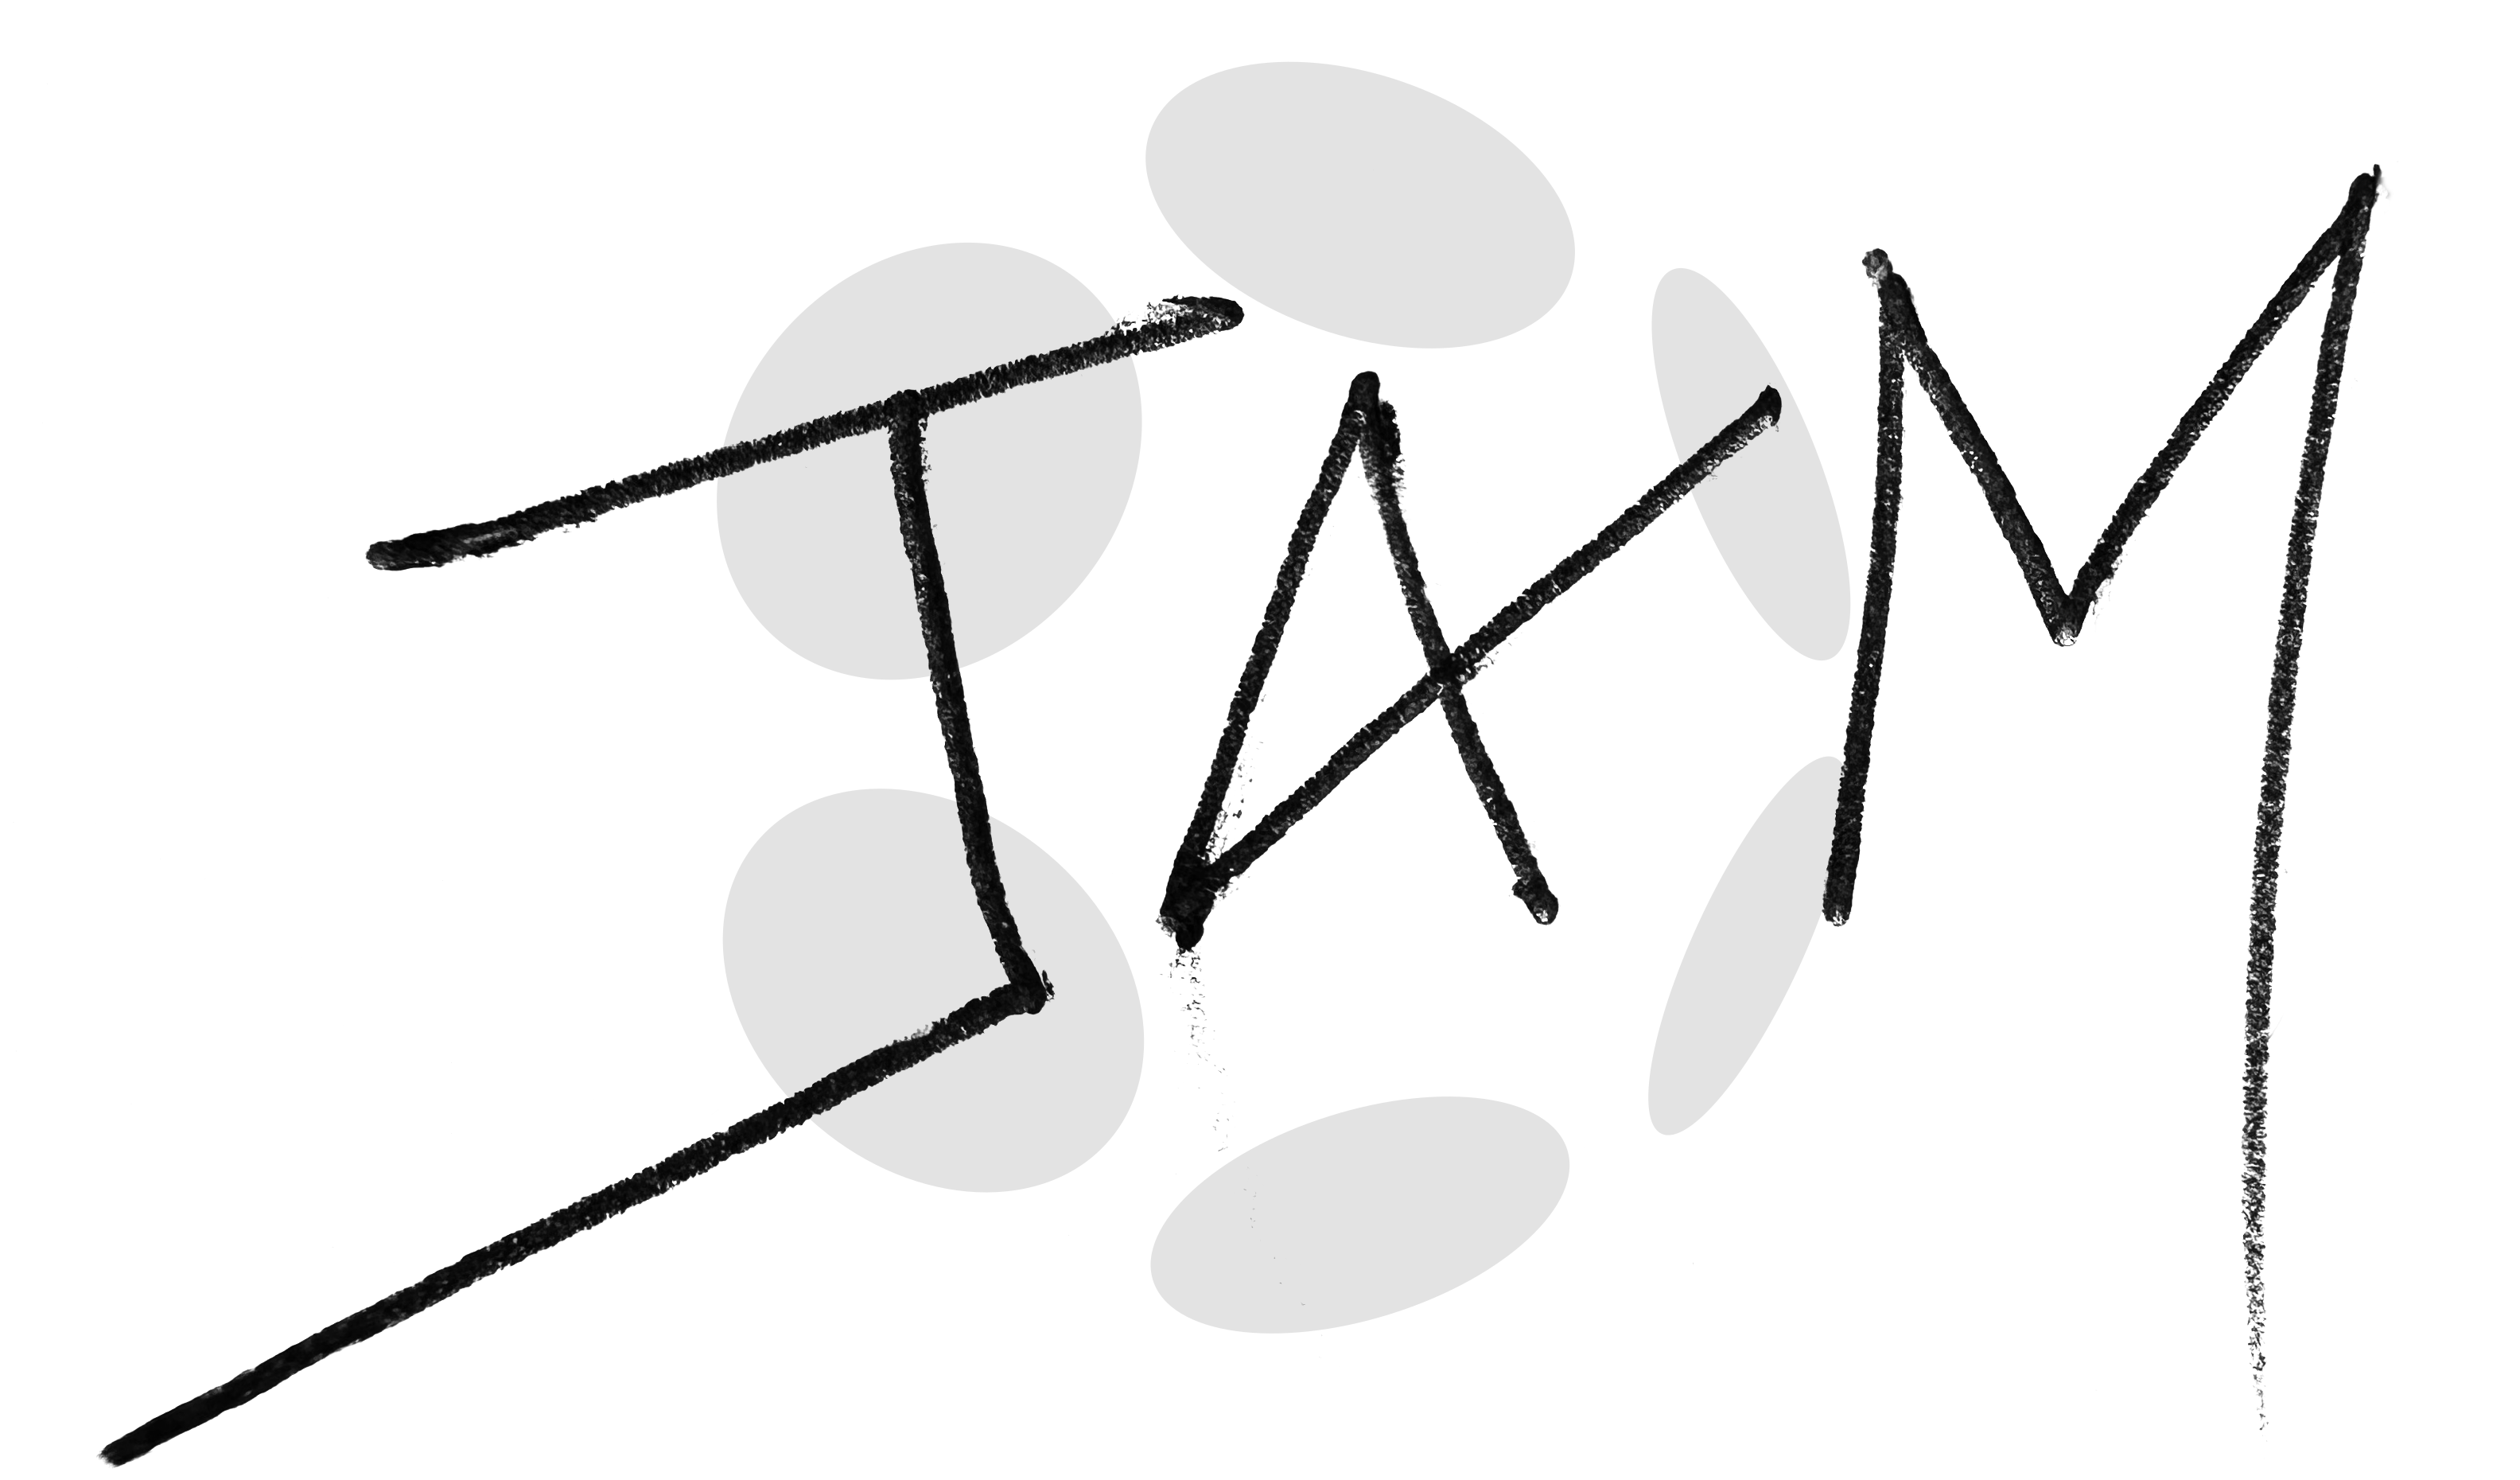
\includegraphics[width=\columnwidth]{assets/jam-pen-back-inverted.png}
\end{center}

\vskip10pt
\maketitle

\section{Introduction}

\subsection{Nomenclature}

%As its namesake paper pointed out, the name \emph{Polkadot} means several things depending on context. It might mean variously the product vision set forth in said paper of a scalable heterogeneous multichain; the decentralized blockchain network and service which came to be along with its state and history; or possibly the protocol and technology-base utilized in order to maintain and run this network and others such as \emph{Kusama}.

In this paper, we introduce a decentralized, crypto-economic protocol to which the Polkadot Network could conceivably transition itself in a major revision. Following this eventuality (which must not be taken for granted since Polkadot is a decentralized network) this protocol might also become known as \emph{Polkadot} or some derivation thereof. However, at this stage this is not the case, therefore our proposed protocol will for the present be known as \Jam.

An early, unrefined, version of this protocol was first proposed in Polkadot Fellowship \textsc{rfc}\oldstylenums{31}, known as \emph{CoreJam}. CoreJam takes its name after the collect/refine/join/accumulate model of computation at the heart of its service proposition. While the CoreJam \textsc{rfc} suggested an incomplete, scope-limited alteration to the Polkadot protocol, \Jam refers to a complete and coherent overall blockchain protocol.

\subsection{Driving Factors}

Within the realm of blockchain and the wider Web3, we are driven by the need first and foremost to deliver resilience. A proper Web3 digital system should honor a declared service profile---and ideally meet even perceived expectations---regardless of the desires, wealth or power of any economic actors including individuals, organizations and, indeed, other Web3 systems. Inevitably this is aspirational, and we must be pragmatic over how perfectly this may really be delivered. Nonetheless, a Web3 system should aim to provide such radically strong guarantees that, for practical purposes, the system may be described as \emph{unstoppable}.

While Bitcoin is, perhaps, the first example of such a system within the economic domain, it was not general purpose in terms of the nature of the service it offered. A rules-based service is only as useful as the generality of the rules which may be conceived and placed within it. Bitcoin's rules allowed for an initial use-case, namely a fixed-issuance token, ownership of which is well-approximated and autonomously enforced through knowledge of a secret, as well as some further elaborations on this theme.

Later, Ethereum would provide a categorically more general-purpose rule set, one which was practically Turing complete.\footnote{The gas mechanism did restrict what programs can execute on it by placing an upper bound on the number of steps which may be executed, but some restriction to avoid infinite-computation must surely be introduced in a permissionless setting.} In the context of Web3 where we are aiming to deliver a massively multiuser application platform, generality is crucial, and thus we take this as a given.

Beyond resilience and generality, things get more interesting, and we must look a little deeper to understand what our driving factors are. For the present purposes, we identify three additional goals:
\begin{enumerate}
  \item \label{enum:resilience} Resilience: highly resistant from being stopped, corrupted and censored.
  \item \label{enum:generality} Generality: able to perform Turing-complete computation.
  \item \label{enum:performance} Performance: able to perform computation quickly and at low cost.
  \item \label{enum:coherency} Coherency: the causal relationship possible between different elements of state and thus how well individual applications may be composed.
  \item \label{enum:accessibility} Accessibility: negligible barriers to innovation; easy, fast, cheap and permissionless.
\end{enumerate}

As a declared Web3 technology, we make an implicit assumption of the first two items. Interestingly, items \ref{enum:performance} and \ref{enum:coherency} are antagonistic according to an information theoretic principle which we are sure must already exist in some form but are nonetheless unaware of a name for it. For argument's sake we shall name it \emph{size-synchrony antagonism}.

\subsection{Scaling under Size-Synchrony Antagonism}

Size-synchrony antagonism is a simple principle implying that as the state-space of information systems grow, then the system necessarily becomes less synchronous. The argument goes:

\begin{enumerate}
  \item The more state a system utilizes for its data-processing, the greater the amount of space this state must occupy.
  \item The more space used, then the greater the mean and variance of distances between state-components.
  \item As the mean and variance increase, then interactions become slower and subsystems must manage the possibility that distances between interdependent components of state could be materially different, requiring asynchrony.
\end{enumerate}

This assumes perfect coherency of the system's state. Setting the question of overall security aside for a moment, we can avoid this rule by applying the \emph{divide and conquer} maxim and fragmenting the state of a system, sacrificing its coherency. We might for example create two independent smaller-state systems rather than one large-state system. This pattern applies a step-curve to the principle; intra-system processing has low size and high synchrony, inter-system processing has high size but low synchrony. It is the principle behind meta-networks such as Polkadot, Cosmos and the predominant vision of a scaled Ethereum (all to be discussed in depth shortly).

The present work explores a middle-ground in the antagonism, avoiding the persistent fragmentation of state-space of the system as with existing approaches. We do this by introducing a new model of computation which pipelines a highly scalable element to a highly synchronous element. Asynchrony is not avoided, but we do open the possibility for a greater degree of granularity over how it is traded against size. In particular fragmentation can be made ephemeral rather than persistent, drawing upon a coherent state and fragmenting it only for as long as it takes to execute any given piece of processing on it.

Unlike with \textsc{snark}-based L2-blockchain techniques for scaling, this model draws upon crypto-economic mechanisms and inherits their low-cost and high-performance profiles and averts a bias toward centralization.

\subsection{Document Structure}

We begin with a brief overview of present scaling approaches in blockchain technology in section \ref{sec:previouswork}. In section \ref{sec:notation} we define and clarify the notation from which we will draw for our formalisms.

We follow with a broad overview of the protocol in section \ref{sec:overview} outlining the major areas including the Polka Virtual Machine (\textsc{pvm}), the consensus protocols Safrole and \textsc{Grandpa}, the common clock and build the foundations of the formalism.

We then continue with the full protocol definition split into two parts: firstly the correct on-chain state-transition formula helpful for all nodes wishing to validate the chain state, and secondly, in sections \ref{sec:workpackagesandworkreports} and \ref{sec:bestchain} the honest strategy for the off-chain actions of any actors who wield a validator key.

The main body ends with a discussion over the performance characteristics of the protocol in section \ref{sec:discussion} and finally conclude in section \ref{sec:conclusion}.

The appendix contains various additional material important for the protocol definition including the \textsc{pvm} in appendices \ref{sec:virtualmachine} \& \ref{sec:virtualmachineinvocations}, serialization and Merklization in appendices \ref{sec:serialization} \& \ref{sec:statemerklization} and cryptography in appendices \ref{sec:merklization}, \ref{sec:bandersnatch} \& \ref{sec:erasurecoding}. We finish with an index of terms which includes the values of all simple constant terms used in the work in appendix \ref{sec:definitions}, and close with the bibliography.
\section{Previous Work and Present Trends}\label{sec:previouswork}

In the years since the initial publication of the Ethereum \emph{YP}, the field of blockchain development has grown immensely. Other than scalability, development has been done around underlying consensus algorithms, smart-contract languages and machines and overall state environments. While interesting, these latter subjects are mostly out scope of the present work since they generally do not impact underlying scalability.

\subsection{Polkadot}

In order to deliver its service, \Jam co-opts much of the same game-theoretic and cryptographic machinery as Polkadot known as \textsc{Elves} and described by \cite{cryptoeprint:2024/961}. However, major differences exist in the actual service offered with \Jam, providing an abstraction much closer to the actual computation model generated by the validator nodes its economy incentivizes.

It was a major point of the original Polkadot proposal, a scalable heterogeneous multichain, to deliver high-performance through partition and distribution of the workload over multiple host machines. In doing so it took an explicit position that composability would be lowered. Polkadot's constituent components, parachains are, practically speaking, highly isolated in their nature. Though a message passing system (\textsc{xcmp}) exists it is asynchronous, coarse-grained and practically limited by its reliance on a high-level slowly evolving interaction language \textsc{xcm}.

As such, the composability offered by Polkadot between its constituent chains is lower than that of Ethereum-like smart-contract systems offering a single and universal object environment and allowing for the kind of agile and innovative integration which underpins their success. Polkadot, as it stands, is a collection of independent ecosystems with only limited opportunity for collaboration, very similar in ergonomics to bridged blockchains though with a categorically different security profile. A technical proposal known as \textsc{spree} would utilize Polkadot's unique shared-security and improve composability, though blockchains would still remain isolated.

Implementing and launching a blockchain is hard, time-consuming and costly. By its original design, Polkadot limits the clients able to utilize its service to those who are both able to do this and raise a sufficient deposit to win an auction for a long-term slot, one of around 50 at the present time. While not permissioned per se, accessibility is categorically and substantially lower than for smart-contract systems similar to Ethereum.

Enabling as many innovators to participate and interact, both with each other and each other's user-base, appears to be an important component of success for a Web3 application platform. Accessibility is therefore crucial.

\subsection{Ethereum}

The Ethereum protocol was formally defined in this paper's spiritual predecessor, the \emph{Yellow Paper}, by \cite{wood2014ethereum}. This was derived in large part from the initial concept paper by \cite{buterin2013ethereum}. In the decade since the \emph{YP} was published, the \emph{de facto} Ethereum protocol and public network instance have gone through a number of evolutions, primarily structured around introducing flexibility via the transaction format and the instruction set and ``precompiles'' (niche, sophisticated bonus instructions) of its scripting core, the Ethereum virtual machine (\textsc{evm}).

Almost one million crypto-economic actors take part in the validation for Ethereum.\footnote{Practical matters do limit the level of real decentralization. Validator software expressly provides functionality to allow a single instance to be configured with multiple key sets, systematically facilitating a much lower level of actual decentralization than the apparent number of actors, both in terms of individual operators and hardware. Using data collated by \cite{hildobby2024eth2} on Ethereum 2, one can see one major node operator, Lido, has steadily accounted for almost one-third of the almost one million crypto-economic participants.} Block extension is done through a randomized leader-rotation method where the physical address of the leader is public in advance of their block production.\footnote{Ethereum's developers hope to change this to something more secure, but no timeline is fixed.} Ethereum uses Casper-FFG introduced by \cite{buterin2019casper} to determine finality, which with the large validator base finalizes the chain extension around every 13 minutes.

Ethereum's direct computational performance remains broadly similar to that with which it launched in 2015, with a notable exception that an additional service now allows 1\textsc{mb} of \emph{commitment data} to be hosted per block (all nodes to store it for a limited period). The data cannot be directly utilized by the main state-transition function, but special functions provide proof that the data (or some subsection thereof) is available. According to \cite{ethereum2024danksharding}, the present design direction is to improve on this over the coming years by splitting responsibility for its storage amongst the validator base in a protocol known as \emph{Dank-sharding}.

According to \cite{ethereum2024sigital}, the scaling strategy of Ethereum would be to couple this data availability with a private market of \emph{roll-ups}, sideband computation facilities of various design, with \textsc{zk-snark}-based roll-ups being a stated preference. Each vendor's roll-up design, execution and operation comes with its own implications.

One might reasonably assume that a diversified market-based approach for scaling via multivendor roll-ups will allow well-designed solutions to thrive. However, there are potential issues facing the strategy. A research report by \cite{sharma2024ethereums} on the level of decentralization in the various roll-ups found a broad pattern of centralization, but notes that work is underway to attempt to mitigate this. It remains to be seen how decentralized they can yet be made.

Heterogeneous communication properties (such as datagram latency and semantic range), security properties (such as the costs for reversion, corruption, stalling and censorship) and economic properties (the cost of accepting and processing some incoming message or transaction) may differ, potentially quite dramatically, between major areas of some grand patchwork of roll-ups by various competing vendors. While the overall Ethereum network may eventually provide some or even most of the underlying machinery needed to do the sideband computation it is far from clear that there would be a ``grand consolidation'' of the various properties should such a thing happen. We have not found any good discussion of the negative ramifications of such a fragmented approach.\footnote{Some initial thoughts on the matter resulted in a proposal by \cite{sadana2024bringing} to utilize Polkadot technology as a means of helping create a modicum of compatibility between roll-up ecosystems!}

\subsubsection{\textsc{Snark} Roll-ups}

While the protocol's foundation makes no great presuppositions on the nature of roll-ups, Ethereum's strategy for sideband computation does centre around \textsc{snark}-based rollups and as such the protocol is being evolved into a design that makes sense for this. \textsc{Snark}s are the product of an area of exotic cryptography which allow proofs to be constructed to demonstrate to a neutral observer that the purported result of performing some predefined computation is correct. The complexity of the verification of these proofs tends to be sub-linear in their size of computation to be proven and will not give away any of the internals of said computation, nor any dependent witness data on which it may rely.

\textsc{Zk-snark}s come with constraints. There is a trade-off between the proof's size, verification complexity and the computational complexity of generating it. Non-trivial computation, and especially the sort of general-purpose computation laden with binary manipulation which makes smart-contracts so appealing, is hard to fit into the model of \textsc{snark}s.

To give a practical example, \textsc{risc}-zero (as assessed by \cite{bogli2024assessing}) is a leading project and provides a platform for producing \textsc{snark}s of computation done by a \textsc{risc-v} virtual machine, an open-source and succinct \textsc{risc} machine architecture well-supported by tooling. A recent benchmarking report by \cite{koute2024risc0} showed that compared to \textsc{risc}-zero's own benchmark, proof generation alone takes over 61,000 times as long as simply recompiling and executing even when executing on 32 times as many cores, using 20,000 times as much \textsc{ram} and an additional state-of-the-art \textsc{gpu}. According to hardware rental agents \url{https://cloud-gpus.com/}, the cost multiplier of proving using \textsc{risc}-zero is 66,000,000x of the cost\footnote{In all likelihood actually substantially more as this was using low-tier ``spare'' hardware in consumer units, and our recompiler was unoptimized.} to execute using our \textsc{risc-v} recompiler.

Many cryptographic primitives become too expensive to be practical to use and specialized algorithms and structures must be substituted. Often times they are otherwise suboptimal. In expectation of the use of \textsc{snark}s (such as \textsc{plonk} as proposed by \cite{cryptoeprint:2019/953}), the prevailing design of the Ethereum project's Dank-sharding availability system uses a form of erasure coding centered around polynomial commitments over a large prime field in order to allow \textsc{snark}s to get acceptably performant access to subsections of data. Compared to alternatives, such as a binary field and Merklization in the present work, it leads to a load on the validator nodes orders of magnitude higher in terms of \textsc{cpu} usage.

In addition to their basic cost, \textsc{snark}s present no great escape from decentralization and the need for redundancy, leading to further cost multiples. While the need for some benefits of staked decentralization is averted through their verifiable nature, the need to incentivize multiple parties to do much the same work is a requirement to ensure that a single party not form a monopoly (or several not form a cartel). Proving an incorrect state-transition should be impossible, however service integrity may be compromised in other ways; a temporary suspension of proof-generation, even if only for minutes, could amount to major economic ramifications for real-time financial applications.

Real-world examples exist of the pit of centralization giving rise to monopolies. One would be the aforementioned \textsc{snark}-based exchange framework; while notionally serving decentralized exchanges, it is in fact centralized with Starkware itself wielding a monopoly over enacting trades through the generation and submission of proofs, leading to a single point of failure---should Starkware's service become compromised, then the liveness of the system would suffer.

It has yet to be demonstrated that \textsc{snark}-based strategies for eliminating the trust from computation will ever be able to compete on a cost-basis with a multi-party crypto-economic platform. All as-yet proposed \textsc{snark}-based solutions are heavily reliant on crypto-economic systems to frame them and work around their issues. Data availability and sequencing are two areas well understood as requiring a crypto-economic solution.

We would note that \textsc{snark} technology is improving and the cryptographers and engineers behind them do expect improvements in the coming years. In a recent article by \cite{thaler2023technical} we see some credible speculation that with some recent advancements in cryptographic techniques, slowdowns for proof generation could be as little as 50,000x from regular native execution and much of this could be parallelized. This is substantially better than the present situation, but still several orders of magnitude greater than would be required to compete on a cost-basis with established crypto-economic techniques such as \textsc{Elves}.

\subsection{Fragmented Meta-Networks}

Directions for general-purpose computation scalability taken by other projects broadly centre around one of two approaches; either what might be termed a \emph{fragmentation} approach or alternatively a \emph{centralization} approach. We argue that neither approach offers a compelling solution.

The fragmentation approach is heralded by projects such as Cosmos (proposed by \cite{kwon2019cosmos}) and Avalanche (by \cite{tanana2019avalanche}). It involves a system fragmented by networks of a homogenous consensus mechanic, yet staffed by separately motivated sets of validators. This is in contrast to Polkadot's single validator set and Ethereum's declared strategy of heterogeneous roll-ups secured partially by the same validator set operating under a coherent incentive framework. The homogeneity of said fragmentation approach allows for reasonably consistent messaging mechanics, helping to present a fairly unified interface to the multitude of connected networks.

However, the apparent consistency is superficial. The networks are trustless only by assuming correct operation of their validators, who operate under a crypto-economic security framework ultimately conjured and enforced by economic incentives and punishments. To do twice as much work with the same levels of security and no special coordination between validator sets, then such systems essentially prescribe forming a new network with the same overall levels of incentivization.

Several problems arise. Firstly, there is a similar downside as with Polkadot's isolated parachains and Ethereum's isolated roll-up chains: a lack of coherency due to a persistently sharded state preventing synchronous composability.

More problematically, the scaling-by-fragmentation approach, proposed specifically by Cosmos, provides no homogenous security---and therefore trustlessness---guarantees. Validator sets between networks must be assumed to be independently selected and incentivized with no relationship, causal or probabilistic, between the Byzantine actions of a party on one network and potential for appropriate repercussions on another. Essentially, this means that should validators conspire to corrupt or revert the state of one network, the effects may be felt across other networks of the ecosystem.

That this is an issue is broadly accepted, and projects propose for it to be addressed in one of two ways. Firstly, to fix the expected cost-of-attack (and thus level of security) across networks by drawing from the same validator set. The massively redundant way of doing this, as proposed by \cite{cosmos2024interchain} under the name \emph{replicated security}, would be to require each validator to validate on all networks and for the same incentives and punishments. This is economically inefficient in the cost of security provision as each network would need to independently provide the same level of incentives and punishment-requirements as the most secure with which it wanted to interoperate. This is to ensure the economic proposition remain unchanged for validators and the security proposition remained equivalent for all networks. At the present time, replicated security is not a readily available permissionless service. We might speculate that these punishing economics have something to do with it.

The more efficient approach, proposed by the OmniLedger team, \cite{cryptoeprint:2017/406}, would be to make the validators non-redundant, partitioning them between different networks and periodically, securely and randomly repartitioning them. A reduction in the cost to attack over having them all validate on a single network is implied since there is a chance of having a single network accidentally have a compromising number of malicious validators even with less than this proportion overall. This aside it presents an effective means of scaling under a basis of weak-coherency.

Alternatively, as in \textsc{Elves} by \cite{cryptoeprint:2024/961}, we may utilize non-redundant partitioning, combine this with a proposal-and-auditing game which validators play to weed out and punish invalid computations, and then require that the finality of one network be contingent on all causally-entangled networks. This is the most secure and economically efficient solution of the three, since there is a mechanism for being highly confident that invalid transitions will be recognized and corrected before their effect is finalized across the ecosystem of networks. However, it requires substantially more sophisticated logic and their causal-entanglement implies some upper limit on the number of networks which may be added.

\subsection{High-Performance Fully Synchronous Networks}

Another trend in the recent years of blockchain development has been to make ``tactical'' optimizations over data throughput by limiting the validator set size or diversity, focusing on software optimizations, requiring a higher degree of coherency between validators, onerous requirements on the hardware which validators must have, or limiting data availability.

The Solana blockchain is underpinned by technology introduced by \cite{yakovenko2018solana} and boasts theoretical figures of over 700,000 transactions per second, though according to \cite{ng2024is} the network is only seen processing a small fraction of this. The underlying throughput is still substantially more than most blockchain networks and is owed to various engineering optimizations in favor of maximizing synchronous performance. The result is a highly-coherent smart-contract environment with an \textsc{api} not unlike that of \emph{YP} Ethereum (albeit using a different underlying \textsc{vm}), but with a near-instant time to inclusion and finality which is taken to be immediate upon inclusion.

Two issues arise with such an approach: firstly, defining the protocol as the outcome of a heavily optimized codebase creates structural centralization and can undermine resilience. \cite{jha2024solana} writes ``since January 2022, 11 significant outages gave rise to 15 days in which major or partial outages were experienced''. This is an outlier within the major blockchains as the vast majority of major chains have no downtime. There are various causes to this downtime, but they are generally due to bugs found in various subsystems.

Ethereum, at least until recently, provided the most contrasting alternative with its well-reviewed specification, clear research over its crypto-economic foundations and multiple clean-room implementations. It is perhaps no surprise that the network very notably continued largely unabated when a flaw in its most deployed implementation was found and maliciously exploited, as described by \cite{hertig2016so}.

The second issue is concerning ultimate scalability of the protocol when it provides no means of distributing workload beyond the hardware of a single machine.

In major usage, both historical transaction data and state would grow impractically. Solana illustrates how much of a problem this can be. Unlike classical blockchains, the Solana protocol offers no solution for the archival and subsequent review of historical data, crucial if the present state is to be proven correct from first principle by a third party. There is little information on how Solana manages this in the literature, but according to \cite{solana2023solana}, nodes simply place the data onto a centralized database hosted by Google.\footnote{Earlier node versions utilized Arweave network, a decentralized data store, but this was found to be unreliable for the data throughput which Solana required.}

Solana validators are encouraged to install large amounts of \textsc{ram} to help hold its large state in memory (512 \textsc{gb} is the current recommendation according to \cite{solana2024solana}). Without a divide-and-conquer approach, Solana shows that the level of hardware which validators can reasonably be expected to provide dictates the upper limit on the performance of a totally synchronous, coherent execution model. Hardware requirements represent barriers to entry for the validator set and cannot grow without sacrificing decentralization and, ultimately, transparency.

\section{Notational Conventions}\label{sec:notation}

Much as in the Ethereum Yellow Paper, a number of notational conventions are used throughout the present work. We define them here for clarity. The Ethereum Yellow Paper itself may be referred to henceforth as the \emph{YP}.

\subsection{Typography}\label{sec:typography}

We use a number of different typefaces to denote different kinds of terms. Where a term is used to refer to a value only relevant within some localized section of the document, we use a lower-case roman letter \eg $x$, $y$ (typically used for an item of a set or sequence) or \eg $i$, $j$ (typically used for numerical indices). Where we refer to a Boolean term or a function in a local context, we tend to use a capitalized roman alphabet letter such as $A$, $F$. If particular emphasis is needed on the fact a term is sophisticated or multidimensional, then we may use a bold typeface, especially in the case of sequences and sets.

For items which retain their definition throughout the present work, we use other typographic conventions. Sets are usually referred to with a blackboard typeface, \eg $\N$ refers to all natural numbers including zero. Sets which may be parameterized may be subscripted or be followed by parenthesized arguments. Imported functions, used by the present work but not specifically introduced by it, are written in calligraphic typeface, \eg $\mathcal{H}$ the Blake2 cryptographic hashing function. For other non-context dependent functions introduced in the present work, we use upper case Greek letters, \eg $\Upsilon$ denotes the state transition function.

Values which are not fixed but nonetheless hold some consistent meaning throughout the present work are denoted with lower case Greek letters such as $\sigma$, the state identifier. These may be placed in bold typeface to denote that they refer to an abnormally complex value.

\subsection{Functions and Operators}\label{sec:functions}
We define the precedes relation to indicate that one term is defined in terms of another. \Eg $y \prec x$ indicates that $y$ may be defined purely in terms of $x$:
\begin{align}\label{eq:precedes}
  y \prec x \Longleftrightarrow \exists f: y = f(x)
\end{align}

%We define $\mathcal{KV}(f)$ to be the set of domain and co-domain element pairs of a function.

%We denote the general fold operator as $\fold$:
%\begin{align}
%  \fold^{S}_{I} F \equiv \begin{cases}
%    I &\when S = [] \\
%    \displaystyle \fold^{[S_1, \dots ]}_{F(I, S_0)} F &\otherwise
%  \end{cases}
%\end{align}

The substitute-if-nothing function $\mathcal{U}$ is equivalent to the first argument which is not $\none$, or $\none$ if no such argument exists:
\begin{align}\label{eq:substituteifnothing}
  \mathcal{U}(a_0, \dots a_n ) \equiv a_x : (a_x \ne \none \vee x = n), \bigwedge_{i=0}^{x-1} a_i = \none
\end{align}
Thus, \eg $\mathcal{U}(\none, 1, \none, 2) = 1$ and $\mathcal{U}(\none, \none) = \none$.

\subsection{Sets}\label{sec:sets}

Given some set $\mathbf{s}$, its power set and cardinality are denoted as the usual $\powset{\mathbf{s}}$ and $|\mathbf{s}|$. When forming a power set, we may use a numeric subscript in order to restrict the resultant expansion to a particular cardinality. \Eg $\powset[2]{\{1, 2, 3\}} = \{ \{1, 2\}, \{1, 3\}, \{2, 3\} \}$.

Sets may be operated on with scalars, in which case the result is a set with the operation applied to each element, \eg $\{1, 2, 3\} + 3 = \{4, 5, 6\}$

We denote set-disjointness with the relation $\disjoint$. Formally:
\begin{equation*}
  A \cap B = \none \Longleftrightarrow A \disjoint B
\end{equation*}

We commonly use $\none$ to indicate that some term is validly left without a specific value. Its cardinality is defined as zero. We define the operation $\bm{?}$ such that $A\bm{?} \equiv A \cup \{\none\}$ indicating the same set but with the addition of the $\none$ element.

The term $\error$ is utilized to indicate the unexpected failure of an operation or that a value is invalid or unexpected. (We try to avoid the use of the more conventional $\bot$ here to avoid confusion with Boolean false, which may be interpreted as some successful result in some contexts.)

\subsection{Numbers}\label{sec:numbers}

$\N$ denotes the set of naturals including zero whereas $\N_n$ implies a restriction on that set to values less than $n$. Formally, $\N = \{0, 1, \dots \}$ and $\N_n = \{ x \mid x \in \N, x < n \}$.

$\mathbb{Z}$ denotes the set of integers. We denote $\mathbb{Z}_{a \dots b}$ to be the set of integers within the interval $[a, b)$. Formally, $\mathbb{Z}_{a \dots b} = \{ x \mid x \in \mathbb{Z}, a \le x < b \}$. \Eg $\mathbb{Z}_{2 \dots 5} = \{ 2, 3, 4 \}$. We denote the offset/length form of this set as $\mathbb{Z}_{a \dots +b}$, a short form of $\mathbb{Z}_{a \dots a+b}$.

It can sometimes be useful to represent lengths of sequences and yet limit their size, especially when dealing with sequences of octets which must be stored practically. Typically, these lengths can be defined as the set $\N_{2^{32}}$. To improve clarity, we denote $\N_L$ as the set of lengths of octet sequences and is equivalent to $\N_{2^{32}}$.

We denote the $\rem$ operator as the modulo operator, \eg $5 \rem 3 = 2$. Furthermore, we may occasionally express a division result as a quotient and remainder with the separator $\remainder$, \eg $5 \div 3 = 1 \remainder 2$.

\subsection{Dictionaries}\label{sec:dictionaries}

A \emph{dictionary} is a possibly partial mapping from some domain into some co-domain in much the same manner as a regular function. Unlike functions however, with dictionaries the total set of pairings are necessarily enumerable, and we represent them in some data structure as the set of all $(key \mapsto value)$ pairs. (In such data-defined mappings, it is common to name the values within the domain a \emph{key} and the values within the co-domain a \emph{value}, hence the naming.)

Thus, we define the formalism $\dict{\mathrm{K}}{\mathrm{V}}$ to denote a dictionary which maps from the domain $\mathrm{K}$ to the range $\mathrm{V}$. We define a dictionary as a member of the set of all dictionaries $\mathbb{D}$ and a set of pairs $p = (k \mapsto v)$:
\begin{align}
  &\mathbb{D} \subset \big \{ \{ (k \mapsto v) \} \big \}
\end{align}

A dictionary's members must associate at most one unique value for any key $k$:
\begin{align}
  \forall \mathbf{d} \in\ &\mathbb{D} : \forall (k \mapsto v) \in \mathbf{d} : \exists! v' : (k \mapsto v') \in \mathbf{d}
\end{align}

This assertion allows us to unambiguously define the subscript and subtraction operator for a dictionary $d$:
\begin{align}
  \forall \mathbf{d} \in \mathbb{D}&: \mathbf{d}[k] \equiv \begin{cases}
    v & \text{if}\ \exists k : (k \mapsto v) \in \mathbf{d} \\
    \none & \otherwise
  \end{cases}\\
  \forall \mathbf{d} \in \mathbb{D}&, \mathbf{s} \subseteq K: \mathbf{d} \setminus \mathbf{s} \equiv \{ (k \mapsto v): (k \mapsto v) \in \mathbf{d}, k \not \in \mathbf{s} \}
\end{align}

Note that when using a subscript, it is an implicit assertion that the key exists in the dictionary. Should the key not exist, the result is undefined and any block which relies on it must be considered invalid.

It is typically useful to limit the sets from which the keys and values may be drawn. Formally, we define a typed dictionary $\dict{K}{V}$ as a set of pairs $p$ of the form $(k \mapsto v)$:
\begin{align}
  \dict{K}{V} &\subset \mathbb{D} \\
  \dict{K}{V} &\equiv \big \{ \{ (k \mapsto v) \mid k \in K \wedge v \in V \} \big \}
\end{align}

To denote the active domain (\ie set of keys) of a dictionary $\mathbf{d} \in \dict{K}{V}$, we use $\keys{\mathbf{d}} \subseteq K$ and for the range (\ie set of values), $\mathcal{V}(\mathbf{d}) \subseteq V$. Formally:
\begin{align}
  \keys{\mathbf{d} \in \mathbb{D}} &\equiv \{\ k \mid \exists v : (k \mapsto v) \in \mathbf{d}\ \} \\
  \mathcal{V}(\mathbf{d} \in \mathbb{D}) &\equiv \{\ v \mid \exists k : (k \mapsto v) \in \mathbf{d}\ \}
\end{align}

Note that since the co-domain of $\mathcal{V}$ is a set, should different keys with equal values appear in the dictionary, the set will only contain one such value.

\subsection{Tuples}\label{sec:tuples}

Tuples are groups of values where each item may belong to a different set. They are denoted with parentheses, \eg the tuple $t$ of the naturals $3$ and $5$ is denoted $t = (3, 5)$, and it exists in the set of natural pairs sometimes denoted $\N \times \N$, but denoted in the present work as $(\N, \N)$.

We have frequent need to refer to a specific item within a tuple value and as such find it convenient to declare a name for each item. \Eg we may denote a tuple with two named natural components $a$ and $b$ as $T = \ltuple\isa{a}{\N}\ts\isa{b}{\N}\rtuple$. We would denote an item $t \in T$ through subscripting its name, thus for some $t = \ltup\is{a}{3}\ts\is{b}{5}\rtup$, $t_a = 3$ and $t_b = 5$.

\subsection{Sequences}\label{sec:sequences}

A sequence is a series of elements with particular ordering not dependent on their values. The set of sequences of elements all of which are drawn from some set $T$ is denoted $\seq{T}$, and it defines a partial mapping $\N \to T$. The set of sequences containing exactly $n$ elements each a member of the set $T$ may be denoted $\seq{T}_n$ and accordingly defines a complete mapping $\N_n \to T$. Similarly, sets of sequences of at most $n$ elements and at least $n$ elements may be denoted $\seq{T}_{:n}$ and $\seq{T}_{n:}$ respectively.

Sequences are subscriptable, thus a specific item at index $i$ within a sequence $\mathbf{s}$ may be denoted $\mathbf{s}[i]$, or where unambiguous, $\mathbf{s}_i$. A range may be denoted using an ellipsis for example: $[0, 1, 2, 3]_{\dots2} = [0, 1]$ and $[0, 1, 2, 3]_{1\dots+2} = [1, 2]$. The length of such a sequence may be denoted $|\mathbf{s}|$.

We denote modulo subscription as $\mathbf{s}[i]^\circlearrowleft \equiv \mathbf{s}[\,i \rem |\mathbf{s}|\,]$. We denote the final element $x$ of a sequence $\mathbf{s} = \sq{..., x}$ through the function $\text{last}(\mathbf{s}) \equiv x$.

\subsubsection{Construction}
We may wish to define a sequence in terms of incremental subscripts of other values: $[\mathbf{x}_0, \mathbf{x}_1, \dots ]_n$ denotes a sequence of $n$ values beginning $\mathbf{x}_0$ continuing up to $\mathbf{x}_{n-1}$. Furthermore, we may also wish to define a sequence as elements each of which are a function of their index $i$; in this case we denote $[f(i) \mid i \orderedin \N_n] \equiv [f(0), f(1), \dots, f(n - 1)]$. Thus, when the ordering of elements matters we use $\orderedin$ rather than the unordered notation $\in$. The latter may also be written in short form $[f(i \orderedin \N_n)]$. This applies to any set which has an unambiguous ordering, particularly sequences, thus $[\,i^2 \mid i \orderedin [1, 2, 3]\,] = [1, 4, 9]$. Multiple sequences may be combined, thus $[\,i\cdot j \mid i \orderedin [1, 2, 3], j \orderedin [2, 3, 4]\,] = [2, 6, 12]$.

We use explicit notation $f^{\#}$ to denote a function mapping over all items of a sequence. Thus given some function $y = f(x)$:
\begin{equation}
  [f(\mathbf{x}_0), f(\mathbf{x}_1), \dots] = f^{\#}([\mathbf{x}_0, \mathbf{x}_1, \dots])
\end{equation}

Sequences may be constructed from sets or other sequences whose order should be ignored through sequence ordering notation $\orderby{i_k}{i \in X}$, which is defined to result in the set or sequence of its argument except that all elements $i$ are placed in ascending order of the corresponding value $i_k$.

The key component may be elided in which case it is assumed to be ordered by the elements directly; \ie $\order{i \in X} \equiv \orderby{i}{i \in X}$. $\orderuniqby{i_k}{i \in X}$ does the same, but excludes any duplicate values of $i$. \Eg assuming $\mathbf{s} = [1, 3, 2, 3]$, then $\orderuniqby{i}{i \in \mathbf{s}} = [ 1, 2, 3 ]$ and $\orderby{-i}{i \in \mathbf{s}} = [ 3, 3, 2, 1 ]$.

Sets may be constructed from sequences with the regular set construction syntax, \eg assuming $\mathbf{s} = [1, 2, 3, 1]$, then $\{ a \mid a \in \mathbf{s} \}$ would be equivalent to $\{ 1, 2, 3 \}$.

Sequences of values which themselves have a defined ordering have an implied ordering akin to a regular dictionary, thus $[1, 2, 3] < [1, 2, 4]$ and $[1, 2, 3] < [1, 2, 3, 1]$.

\subsubsection{Editing}
We define the sequence concatenation operator $\frown$ such that $[\mathbf{x}_0, \mathbf{x}_1, \dots, \mathbf{y}_0, \mathbf{y}_1, \dots] \equiv \mathbf{x} \frown \mathbf{y}$. For sequences of sequences, we define a unary concatenate-all operator: $\wideparen{\mathbf{x}}\equiv\mathbf{x}_0 \frown \mathbf{x}_1 \frown \dots$. Further, we denote element concatenation as $x \doubleplus i \equiv x \frown [i]$. We denote the sequence made up of the first $n$ elements of sequence $\mathbf{s}$ to be ${\overrightarrow{\mathbf{s}}}^n \equiv [\mathbf{s}_0, \mathbf{s}_1, \dots, \mathbf{s}_{n-1}]$, and only the final elements as ${\overleftarrow{\mathbf{s}}}^n$.

We define ${}^\text{T}\mathbf{x}$ as the transposition of the sequence-of-sequences $\mathbf{x}$, fully defined in equation \ref{eq:transpose}. We may also apply this to sequences-of-tuples to yield a tuple of sequences.

We denote sequence subtraction with a slight modification of the set subtraction operator; specifically, some sequence $\mathbf{s}$ excepting the left-most element equal to $v$ would be denoted $\mathbf{s}\seqminusl\{v\}$.

\subsubsection{Boolean values}
$\mathbb{B}_s$ denotes the set of Boolean strings of length $s$, thus $\mathbb{B}_s = \seq{\{\bot, \top\}}_s$. When dealing with Boolean values we may assume an implicit equivalence mapping to a bit whereby $\top = 1$ and $\bot = 0$, thus $\mathbb{B}_\Box = \seq{\N_2}_\Box$. We use the function $\text{bits}(\Y) \in \mathbb{B}$ to denote the sequence of bits, ordered with the least significant first, which represent the octet sequence $\Y$, thus $\text{bits}([5, 0]) = [1, 0, 1, 0, 0, \dots]$.

\subsubsection{Octets and Blobs}

$\Y$ denotes the set of octet strings (``blobs'') of arbitrary length. As might be expected, $\Y_x$ denotes the set of such sequences of length $x$. $\Y_\$$ denotes the subset of $\Y$ which are ASCII-encoded strings. Note that while an octet has an implicit and obvious bijective relationship with natural numbers less than 256, and we may implicitly coerce between octet form and natural number form, we do not treat them as exactly equivalent entities. In particular for the purpose of serialization, an octet is always serialized to itself, whereas a natural number may be serialized as a sequence of potentially several octets, depending on its magnitude and the encoding variant.

\subsubsection{Shuffling}

We define the sequence-shuffle function $\mathcal{F}$, originally introduced by \cite{fisheryates1938statistical}, with an efficient in-place algorithm described by \cite{wikipedia2024fisheryates}. This accepts a sequence and some entropy and returns a sequence of the same length with the same elements but in an order determined by the entropy. The entropy may be provided as either an indefinite sequence of naturals or a hash. For a full definition see appendix \ref{sec:shuffle}.

\subsection{Cryptography}\label{sec:cryptography}

\subsubsection{Hashing}

$\H$ denotes the set of 256-bit values typically expected to be arrived at through a cryptographic function, equivalent to $\Y_{32}$, with $\H^0$ being equal to $[0]_{32}$. We assume a function $\mathcal{H}(m \in \Y) \in \H$ denoting the Blake2b 256-bit hash introduced by \cite{rfc7693} and a function $\mathcal{H}_K(m \in \Y) \in \H$ denoting the Keccak 256-bit hash as proposed by \cite{bertoni2013keccak} and utilized by \cite{wood2014ethereum}.

We may sometimes wish to take only the first $x$ octets of a hash, in which case we denote $\mathcal{H}_x(m) \in \Y_x$ to be the first $x$ octets of $\mathcal{H}(m)$. The inputs of a hash function are generally assumed to be serialized with our codec $\mathcal{E}(x) \in \Y$, however for the purposes of clarity or unambiguity we may also explicitly denote the serialization. Similarly, we may wish to interpret a sequence of octets as some other kind of value with the assumed decoder function $\de(x \in \Y)$. In both cases, we may subscript the transformation function with the number of octets we expect the octet sequence term to have. Thus, $r = \mathcal{E}_4(x \in \N)$ would assert $x \in \N_{2^{32}}$ and $r \in \Y_4$, whereas $s = \de_8(y)$ would assert $y \in \Y_8$ and $s \in \N_{2^{64}}$.

\subsubsection{Signing Schemes}\label{sec:signing}

$\sig{k}{m} \subset \Y_{64}$ is the set of valid Ed25519 signatures, defined by \cite{rfc8032}, made through knowledge of a secret key whose public key counterpart is $k \in \Y_{32}$ and whose message is $m$. To aid readability, we denote the set of valid public keys $k \in \H_E$.

We use $\Y_{BLS} \subset \Y_{144}$ to denote the set of public keys for the \textsc{bls} signature scheme, described by \cite{jofc-2004-14130}, on curve \textsc{bls}\oldstylenums{12}-\oldstylenums{381} defined by \cite{bls12-381}.

We denote the set of valid Bandersnatch public keys as $\H_B$, defined in appendix \ref{sec:bandersnatch}. $\bandersig{k \in \H_B}{x \in \Y}{m \in \Y} \subset \Y_{96}$ is the set of valid singly-contextualized signatures of utilizing the secret counterpart to the public key $k$, some context $x$ and message $m$.

$\bandersnatch{r \in \Y_R}{x \in \Y}{m \in \Y} \subset \Y_{784}$, meanwhile, is the set of valid Bandersnatch Ring\textsc{vrf} deterministic singly-contextualized proofs of knowledge of a secret within some set of secrets identified by some root in the set of valid \emph{roots} $\Y_R \subset \Y_{144}$. We denote $\mathcal{O}(\mathbf{s} \in \seq{\H_B}) \in \Y_R$ to be the root specific to the set of public key counterparts $\mathbf{s}$. A root implies a specific set of Bandersnatch key pairs, knowledge of one of the secrets would imply being capable of making a unique, valid---and anonymous---proof of knowledge of a unique secret within the set.

Both the Bandersnatch signature and Ring\textsc{vrf} proof strictly imply that a member utilized their secret key in combination with both the context $x$ and the message $m$; the difference is that the member is identified in the former and is anonymous in the latter. Furthermore, both define a \textsc{vrf} \emph{output}, a high entropy hash influenced by $x$ but not by $m$, formally denoted $\banderout{\bandersnatch{r}{x}{m}} \subset \H$ and $\banderout{\bandersig{k}{x}{m}} \subset \H$.

We define the function $\mathcal{S}$ as the signature function, such that $\mathcal{S}_{k}(m) \in \bandersig{k}{[]}{m} \cup \sig{k}{m}$. We assert that the ability to compute a result for this function relies on knowledge of a secret key.

\section{Overview}\label{sec:overview}

As in the Yellow Paper, we begin our formalisms by recalling that a blockchain may be defined as a pairing of some initial state together with a block-level state-transition function. The latter defines the posterior state given a pairing of some prior state and a block of data applied to it. Formally, we say:
\begin{align}\label{eq:statetransition}
\sigma' \equiv \Upsilon(\sigma, \mathbf{B})
\end{align}

Where $\sigma$ is the prior state, $\sigma'$ is the posterior state, $B$ is some valid block and $\Upsilon$ is our block-level state-transition function.

Broadly speaking, \Jam (and indeed blockchains in general) may be defined simply by specifying $\Upsilon$ and some \emph{genesis state} $\sigma^0$.\footnote{Practically speaking, blockchains sometimes make assumptions of some fraction of participants whose behavior is simply \emph{honest}, and not provably incorrect nor otherwise economically disincentivized. While the assumption may be reasonable, it must nevertheless be stated apart from the rules of state-transition.} We also make several additional assumptions of agreed knowledge: a universally known clock, and the practical means of sharing data with other systems operating under the same consensus rules. The latter two were both assumptions silently made in the \emph{YP}.

\subsection{The Block}

To aid comprehension and definition of our protocol, we partition as many of our terms as possible into their functional components. We begin with the block $B$ which may be restated as the header $H$ and some input data external to the system and thus said to be \emph{extrinsic}, $\mathbf{E}$:
\begin{align}
  \label{eq:block}\mathbf{B} &\equiv (\mathbf{H}, \mathbf{E}) \\
  \label{eq:extrinsic}\mathbf{E} &\equiv (\mathbf{E}_T, \mathbf{E}_J, \mathbf{E}_P, \mathbf{E}_A, \mathbf{E}_G)
\end{align}

The header is a collection of metadata primarily concerned with cryptographic references to the blockchain ancestors and the operands and result of the present transition. As an immutable known \emph{a priori}, it is assumed to be available throughout the functional components of block transition. The extrinsic data is split into its several portions:

\begin{description}
  \item[tickets] Tickets, used for the mechanism which manages the selection of validators for the permissioning of block authoring. This component is denoted $\mathbf{E}_T$.
  \item[judgements] Votes, by validators, on dispute(s) arising between them presently taking place. This is denoted $\mathbf{E}_J$.
  \item[preimages] Static data which is presently being requested to be available for workloads to be able to fetch on demand. This is denoted $\mathbf{E}_P$.
  \item[availability] Assurances by each validator concerning which of the input data of workloads they have correctly received and are storing locally. This is denoted $\mathbf{E}_A$.
  \item[reports] Reports of newly completed workloads whose accuracy is guaranteed by specific validators. This is denoted $\mathbf{E}_G$.
\end{description}

\subsection{The State}

Our state may be logically partitioned into several largely independent segments which can both help avoid visual clutter within our protocol description and provide formality over elements of computation which may be simultaneously calculated (i.e. parallelized). We therefore pronounce an equivalence between $\sigma$ (some complete state) and a tuple of partitioned segments of that state:
\begin{align}\label{eq:statecomposition}
  \sigma &\equiv (\alpha, \beta, \gamma, \delta, \eta, \iota, \kappa, \lambda, \rho, \tau, \varphi, \chi, \psi, \pi)
\end{align}

In summary, $\delta$ is the portion of state dealing with \emph{services}, analogous in \Jam to the Yellow Paper's (smart contract) \emph{accounts}, the only state of the \emph{YP}'s Ethereum. The identities of services which hold some privileged status are tracked in $\chi$.

Validators, who are the set of economic actors uniquely privileged to help build and maintain the \Jam chain, are identified within $\kappa$, archived in $\lambda$ and enqueued from $\iota$. All other state concerning the determination of these keys is held within $\gamma$. Note this is a departure from the \emph{YP} proof-of-work definitions which were mostly stateless, and this set was not enumerated but rather limited to those with sufficient compute power to find a partial hash-collision in the \textsc{sha}\oldstylenums{2}-\oldstylenums{256} cryptographic hash function. An on-chain entropy pool is retained in $\eta$.

Our state also tracks two aspects of each core: $\alpha$, the authorization requirement which work done on that core must satisfy at the time of being reported on-chain, together with the queue which fills this, $\varphi$; and $\rho$, each of the cores' currently assigned \emph{report}, the availability of whose \emph{work-package} must yet be assured by a super-majority of validators.

Finally, details of the most recent blocks and time are tracked in $\beta$ and $\tau$ respectively and, judgements are tracked in $\psi$ and validator statistics are tracked in $\pi$.

\subsubsection{State Transition Dependency Graph}

Much as in the \emph{YP}, we specify $\Upsilon$ as the implication of formulating all items of posterior state in terms of the prior state and block. To aid the architecting of implementations which parallelize this computation, we minimize the depth of the dependency graph where possible. The overall dependency graph is specified here:
\begin{align}\label{eq:transitionfunctioncomposition}
  \tau' &\prec \mathbf{H} \\
  \beta^\dagger &\prec (\mathbf{H}, \beta) \label{eq:betadagger} \\
  \beta' &\prec (\mathbf{H}, \mathbf{E}_G, \beta^\dagger, \mathbf{C}) \\
  \gamma' &\prec (\mathbf{H}, \tau, \mathbf{E}_T, \gamma, \iota, \eta', \kappa') \\
  \eta' &\prec (\mathbf{H}, \tau, \eta) \\
  \kappa' &\prec (\mathbf{H}, \tau, \kappa, \gamma, \psi') \\
  \lambda' &\prec (\mathbf{H}, \tau, \lambda, \kappa) \\
  \psi' &\prec (\mathbf{E}_J, \psi) \\
  \delta^\dagger &\prec (\mathbf{E}_P, \delta, \tau') \label{eq:deltadagger} \\
  \rho^\dagger &\prec (\mathbf{E}_J, \rho) \label{eq:rhodagger} \\
  \rho^\ddagger &\prec (\mathbf{E}_A, \rho^\dagger) \label{eq:rhoddagger} \\
  \rho' &\prec (\mathbf{E}_G, \rho^\ddagger, \kappa, \tau') \\
  \begin{rcases*}
    \delta' \\
    \chi' \\
    \iota' \\
    \varphi' \\
    \mathbf{C}
  \end{rcases*} &\prec (\mathbf{E}_A, \rho', \delta^\dagger, \chi, \iota, \varphi) \\
  \alpha' &\prec (\mathbf{E}_G, \varphi', \alpha) \\
  \pi' &\prec (\mathbf{E}_G, \mathbf{E}_P, \mathbf{E}_A, \mathbf{E}_T, \tau, \tau', \pi)
\end{align}

The only synchronous entanglements are visible through the intermediate components superscripted with a dagger and defined in equations \ref{eq:betadagger}, \ref{eq:deltadagger} and \ref{eq:rhoddagger}. The latter two mark a merge and join in the dependency graph and, concretely, imply that the preimage lookup extrinsic must be folded into state before the availability extrinsic may be fully processed and accumulation of work happen.

\subsection{Which History?}

A blockchain is a sequence of blocks, each cryptographically referencing some prior block by including a hash of its header, all the way back to some first block which references the genesis header. We already presume consensus over this genesis header $\mathbf{H}^0$ and the state it represents already defined as $\sigma^0$.

By defining a deterministic function for deriving a single posterior state for any (valid) combination of prior state and block, we are able to define a unique \emph{canonical} state for any given block. We generally call the block with the most ancestors the \emph{head} and its state the \emph{head state}.

It is generally possible for two blocks to be valid and yet reference the same prior block in what is known as a \emph{fork}. This implies the possibility of two different heads, each with their own state. While we know of no way to strictly preclude this possibility, for the system to be useful we must nonetheless attempt to minimize it. We therefore strive to ensure that:

\begin{enumerate}
  \item\label{enum:wh:minimize} It be generally unlikely for two heads to form.
  \item\label{enum:wh:resolve} When two heads do form they be quickly resolved into a single head.
  \item\label{enum:wh:finalize} It be possible to identify a block not much older than the head which we can be extremely confident will form part of the blockchain's history in perpetuity. When a block becomes identified as such we call it \emph{finalized} and this property naturally extends to all of its ancestor blocks.
\end{enumerate}

These goals are achieved through a combination of two consensus mechanisms: \emph{Safrole}, which governs the (not-necessarily forkless) extension of the blockchain; and \emph{Grandpa}, which governs the finalization of some extension into canonical history. Thus, the former delivers point \ref{enum:wh:minimize}, the latter delivers point \ref{enum:wh:finalize} and both are important for delivering point \ref{enum:wh:resolve}. We describe these portions of the protocol in detail in sections \ref{sec:blockproduction} and \ref{sec:grandpa} respectively.

While Safrole limits forks to a large extent (through cryptography, economics and common-time, below), there may be times when we wish to intentionally fork since we have come to know that a particular chain extension must be reverted. In regular operation this should never happen, however we cannot discount the possibility of malicious or malfunctioning nodes. We therefore define such an extension as any which contains a block in which data is reported which \emph{any other} block's state has tagged as invalid (see section \ref{sec:judgements} on how this is done). We further require that Grandpa not finalize any extension which contains such a block. See section \ref{sec:bestchain} for more information here.

\subsection{Time}\label{sec:commonera}

We presume a pre-existing consensus over time specifically for block production and import. While this was not an assumption of Polkadot, pragmatic and resilient solutions exist including the \textsc{ntp} protocol and network. We utilize this assumption in only one way: we require that blocks be considered temporarily invalid if their timeslot is in the future. This is specified in detail in section \ref{sec:blockproduction}.

Formally, we define the time in terms of seconds passed since the beginning of the \Jam\emph{Common Era}, 1200 UTC on January 1, 2024.\footnote{1,704,110,400 seconds after the Unix Epoch.} Midday CET is selected to ensure that all significant timezones are on the same date at any exact 24-hour multiple from the beginning of the common era. Formally, this value is denoted $\mathcal{T}$.

\subsection{Best block}

Given the recognition of a number of valid blocks, it is necessary to determine which should be treated as the ``best'' block, by which we mean the most recent block we believe will ultimately be within of all future \Jam chains. The simplest and least risky means of doing this would be to inspect the Grandpa finality mechanism which is able to provide a block for which there is a very high degree of confidence it will remain an ancestor to any future chain head.

However, in reducing the risk of the resulting block ultimately not being within the canonical chain, Grandpa will typically return a block some small period older than the most recently authored block. (Existing deployments suggest around 1-2 blocks in the past under regular operation.) There are often circumstances when we may wish to have less latency at the risk of the returned block not ultimately forming a part of the future canonical chain. \Eg we may be in a position of being able to author a block, and we need to decide what its parent should be. Alternatively, we may care to speculate about the most recent state for the purpose of providing information to a downstream application reliant on the state of \Jam.

In these cases, we define the best block as the head of the best chain, itself defined in section \ref{sec:bestchain}.

\subsection{Economics}

The present work describes a crypto-economic system, \ie one combining elements of both cryptography and economics and game theory to deliver a self-sovereign digital service. In order to codify and manipulate economic incentives we define a token which is native to the system, which we will simply call \emph{tokens} in the present work.

A value of tokens is generally referred to as a \emph{balance}, and such a value is said to be a member of the set of balances, $\N_B$, which is exactly equivalent to the set of naturals less than $2^{64}$ (\ie 64-bit unsigned integers in coding parlance). Formally:
\begin{align}\label{eq:balance}
  \N_B \equiv \N_{2^{64}}
\end{align}

Though unimportant for the present work, we presume that there be a standard named denomination for $10^{9}$ tokens. This is different to both Ethereum (which uses a denomination of $10^{18}$), Polkadot (which uses a denomination of $10^{10}$) and Polkadot's experimental cousin Kusama (which uses $10^{12}$).

The fact that balances are constained to being less than $2^{64}$ implies that there may never be more than around $18\times10^{9}$ tokens (each divisible into portions of $10^{-9}$) within \Jam. We would expect that the total number of tokens ever issued will be a substantially smaller amount than this.

We further presume that a number of constant \emph{prices} stated in terms of tokens are known. However we leave the specific values to be determined in following work:

\begin{description}\label{eq:prices}
  \item[$\mathsf{B}_I$] the additional minimum balance implied for a single item within a mapping.
  \item[$\mathsf{B}_L$] the additional minimum balance implied for a single octet of data within a mapping.
  \item[$\mathsf{B}_S$] the minimum balance implied for a service.
\end{description}




















\subsection{The Virtual Machine and Gas}\label{sec:virtualmachineandgas}

In the present work, we presume the definition of a \emph{Polka Virtual Machine} (\textsc{pvm}). This virtual machine is based around the \textsc{risc-v} instruction set architecture, specifically the \textsc{rv}\oldstylenums{32}\textsc{em} variant, and is the basis for introducing permissionless logic into our state-transition function.

The \textsc{pvm} is comparable to the \textsc{evm} defined in the Yellow Paper, but somewhat simpler: the complex instructions for cryptographic operations are missing as are those which deal with environmental interactions. Overall it is far less opinionated since it alters a pre-existing general purpose design, \textsc{risc-v}, and optimizes it for our needs. This gives us excellent pre-existing tooling, since \textsc{pvm} remains essentially compatible with \textsc{risc-v}, including support from the compiler toolkit \textsc{llvm} and languages such as Rust and C++. Furthermore, the instruction set simplicity which \textsc{risc-v} and \textsc{pvm} share, together with the register size (32-bit), active number (13) and endianness (little) make it especially well-suited for creating efficient recompilers on to common hardware architectures.

The \textsc{pvm} is fully defined in appendix \ref{sec:virtualmachine}, but for contextualization we will briefly summarize the basic invocation function $\Psi$ which computes the resultant state of a \textsc{pvm} instance initialized with some registers ($\lseq\N_R\rseq_{13}$) and \textsc{ram} ($\mathbb{M}$) and has executed for up to some amount of gas ($\N_G$), a number of approximately time-proportional computational steps:
\begin{equation}
  \Psi\colon
  \tuple{\,
    \begin{alignedat}{3}
      &\Y\ts\ \ \N_R\ts\ \ &&\N_G\ts\\
      &\!\lseq\N_R\rseq_{13}\ts\ \ &&\mathbb{M}\\
    \end{alignedat}
  \,}
  \to
  \tuple{\,
    \begin{aligned}
      &\{\halt, \panic, \oog\} \cup \{\fault,\host\} \times \N_R,\\
      &\N_R,\ \ \Z_G,\ \ \seq{\N_R}_{13},\ \ \mathbb{M}
    \end{aligned}
  \,}
\end{equation}

We refer to the time-proportional computational steps as \emph{gas} (much like in the \emph{YP}) and limit it to a 64-bit quantity. We may use either $\N_G$ or $\Z_G$ to bound it, the first as a prior argument since it is known to be positive, the latter as a result where a negative value indicates an attempt to execute beyond the gas limit. Within the context of the \textsc{pvm}, $\xi \in \N_G$ is typically used to denote gas.
\begin{equation}\label{eq:gasregentry}
  \Z_G \equiv \mathbb{Z}_{-2^{63}:2^{63}}\ ,\quad
  \N_G \equiv \mathbb{N}_{2^{64}}\ ,\quad
  \N_R \equiv \N_{2^{32}}
\end{equation}

It is left as a rather important implementation detail to ensure that the amount of time taken while computing the function $\Psi(\dots, \xi, \dots)$ has a maximum computation time approximately proportional to the value of $\xi$ regardless of other operands.

The \textsc{pvm} is a very simple \textsc{risc} \emph{register machine} and as such has 13 registers, each of which is a 32-bit quantity, denoted as $\N_R$, a natural less than $2^{32}$.\footnote{This is three fewer than \textsc{risc-v}'s 16, however the amount that program code output by compilers uses is 13 since two are reserved for operating system use and the third is fixed as zero} Within the context of the \textsc{pvm}, $\omega \in \seq{\N_R}_{13}$ is typically used to denote the registers.
\begin{align}
  \mathbb{M} &\equiv \ltuple\isa{\mathbf{V}}{\Y_{2^{32}}}\ts\isa{\mathbf{A}}{\lseq\{\text{W}, \text{R}, \none\}\rseq_{2^{32}}}\rtuple
\end{align}

The \textsc{pvm} assumes a simple pageable \textsc{ram} of 32-bit addressable octets where each octet may be either immutable, mutable or inaccessible. The \textsc{ram} definition $\mathbb{M}$ includes two components: a value $\mathbf{V}$ and access $\mathbf{A}$. If the component is unspecified while being subscripted then the value component may be assumed. Within the context of the virtual machine, $\mu \in \mathbb{M}$ is typically used to denote \textsc{ram}.
\begin{align}
  \mathbb{V}_{\mu} \equiv \{i \mid \mu_\mathbf{A}[i] \ne \none \} \qquad
  \mathbb{V}^*_{\mu} \equiv \{i \mid \mu_\mathbf{A}[i] = \text{W} \}
\end{align}

We define two sets of indices for the \textsc{ram} $\mu$: $\mathbb{V}_{\mu}$ is the set of indices which may be read from; and $\mathbb{V}^*_{\mu}$ is the set of indices which may be written to.

Invocation of the \textsc{pvm} has an exit-reason as the first item in the resultant tuple. It is either:
\begin{itemize}
  \item Regular program termination caused by an explicit halt instruction, $\halt$.
  \item Irregular program termination caused by some exceptional circumstance, $\panic$.
  \item Exhaustion of gas, $\oog$.
  \item A page fault (attempt to access some address in \textsc{ram} which is not accessible), $\fault$. This includes the address at fault.
  \item An attempt at progressing a host-call, $\host$. This allows for the progression and integration of a context-dependent state-machine beyond the regular \textsc{pvm}.
\end{itemize}

The full definition follows in appendix \ref{sec:virtualmachine}.

















\subsection{Epochs and Slots}\label{sec:epochsandslots}

Unlike the \emph{YP} Ethereum with its proof-of-work consensus system, \Jam defines a proof-of-authority consensus mechanism, with the authorized validators presumed to be identified by a set of public keys and decided by a \emph{staking} mechanism residing within some system hosted by \Jam. The staking system is out of scope for the present work; instead there is an \textsc{api} which may be utilized to update these keys, and we presume that whatever logic is needed for the staking system will be introduced and utilize this \textsc{api} as needed.

The Safrole mechanism subdivides time following genesis into fixed length \emph{epoch}s with each epoch divided into $\mathsf{E} = 600$ time\emph{slot}s each of uniform length $\mathsf{P} = 6$ seconds, given an epoch period of $\mathsf{E}\cdot\mathsf{P} = 3600$ seconds or one hour.

This six-second slot period represents the minimum time between \Jam blocks, and through Safrole we aim to strictly minimize forks arising both due to contention within a slot (where two valid blocks may be produced within the same six-second period) and due to contention over multiple slots (where two valid blocks are produced in different time slots but with the same parent).

Formally when identifying a timeslot index, we use a natural less than $2^{32}$ (in compute parlance, a 32-bit unsigned integer) indicating the number of six-second timeslots from the \Jam Common Era. For use in this context we introduce the set $\N_T$:
\begin{align}\label{eq:time}
  \N_T \equiv \N_{2^{32}}
\end{align}

This implies that the lifespan of the proposed protocol takes us to mid-August of the year 2840, which with the current course that humanity is on should be ample.

\subsection{The Core Model and Services}\label{sec:coremodelandservices}

Whereas in the Ethereum Yellow Paper when defining the state machine which is held in consensus amongst all network participants, we presume that all machines maintaining the full network state and contributing to its enlargement---or, at least, hoping to---evaluate all computation. This ``everybody does everything'' approach might be called the \emph{on-chain consensus model}. It is unfortunately not scalable, since the network can only process as much logic in consensus that it could hope any individual node is capable of doing itself within any given period of time.

\subsubsection{In-core Consensus}
In the present work, we achieve scalability of the work done through introducing a second model for such computation which we call the \emph{in-core consensus model}. In this model, and under normal circumstances, only a subset of the network is responsible for actually executing any given computation and assuring the availability of any input data it relies upon to others. By doing this and assuming a certain amount of computational parallelism within the validator nodes of the network, we are able to scale the amount of computation done in consensus commensurate with the size of the network, and not with the computational power of any single machine. In the present work we expect the network to be able to do upwards of 300 times the amount of computation \emph{in-core} as that which could be performed by a single machine running the virtual machine at full speed.

Since in-core consensus is not evaluated or verified by all nodes on the network, we must find other ways to become adequately confident that the results of the computation are correct, and any data used in determining this is available for a practical period of time. We do this through a crypto-economic game of three stages called \emph{guaranteeing}, \emph{assuring}, \emph{auditing} and, potentially, \emph{judging}. Respectively, these attach a substantial economic cost to the invalidity of some proposed computation; then a sufficient degree of confidence that the inputs of the computation will be available for some period of time; and finally, a sufficient degree of confidence that the validity of the computation (and thus enforcement of the first guarantee) will be checked by some party who we can expect to be honest.

All execution done in-core must be reproducible by any node synchronized to the portion of the chain which has been finalized. Execution done in-core is therefore designed to be as stateless as possible. The requirements for doing it include only the refinement code of the service, the code of the authorizer and any preimage lookups it carried out during its execution.

When a work-report is presented on-chain, a specific block known as the \emph{lookup-anchor} is identified. Correct behavior requires that this must be in the finalized chain and reasonably recent, both properties which may be proven and thus are acceptable for use within a consensus protocol.

We describe this pipeline in detail in the relevant sections later.

\subsubsection{On Services and Accounts}

% TODO Move these next two sections elsewhere.

In \emph{YP} Ethereum, we have two kinds of accounts: \emph{contract accounts} (whose actions are defined deterministically based on the account's associated code and state) and \emph{simple accounts} which act as gateways for data to arrive into the world state and are controlled by knowledge of some secret key. In \Jam, all accounts are \emph{service accounts}. Like Ethereum's contract accounts, they have an associated balance, some code and state. Since they are not controlled by a secret key, they do not need a nonce.

The question then arises: how can external data be fed into the world state of \Jam? And, by extension, how does overall payment happen if not by deducting the account balances of those who sign transactions? The answer to the first lies in the fact that our service definition actually includes \emph{multiple} code entry-points, one concerning \emph{refinement} and the other concerning \emph{accumulation}. The former acts as a sort of high-performance stateless processor, able to accept arbitrary input data and distill it into some much smaller amount of output data. The latter code is more stateful, providing access to certain on-chain functionality including the possibility of transferring balance and invoking the execution of code in other services. Being stateful this might be said to more closely correspond to the code of an Ethereum contract account.

To understand how \Jam breaks up its service code is to understand \Jam's fundamental proposition of generality and scalability. All data extrinsic to \Jam is fed into the refinement code of some service. This code is not executed \emph{on-chain} but rather is said to be executed \emph{in-core}. Thus, whereas the accumulator code is subject to the same scalability constraints as Ethereum's contract accounts, refinement code is executed off-chain and subject to no such constraints, enabling \Jam services to scale dramatically both in the size of their inputs and in the complexity of their computation.

While refinement and accumulation take place in consensus environments of a different nature, both are executed by the members of the same validator set. The \Jam protocol through its rewards and penalties ensures that code executed \emph{in-core} has a comparable level of crypto-economic security to that executed \emph{on-chain}, leaving the primary difference between them one of scalability versus synchroneity.

As for managing payment, \Jam introduces a new abstraction mechanism based around Polkadot's Agile Coretime. Within the Ethereum transactive model, the mechanism of account authorization is somewhat combined with the mechanism of purchasing blockspace, both relying on a cryptographic signature to identify a single ``transactor'' account. In \Jam, these are separated and there is no such concept of a ``transactor''.

In place of Ethereum's gas model for purchasing and measuring blockspace, \Jam has the concept of \emph{coretime}, which is prepurchased and assigned to an authorization agent. Coretime is analogous to gas insofar as it is the underlying resource which is being consumed when utilizing \Jam. Its procurement is out of scope in the present work and is expected to be managed by a system parachain operating within a parachains service itself blessed with a number of cores for running such system services. The authorization agent allows external actors to provide input to a service without necessarily needing to identify themselves as with Ethereum's transaction signatures. They are discussed in detail in section \ref{sec:authorization}.

\section{The Header}\label{sec:header}

We must first define the header in terms of its components. The header comprises a parent hash and prior state root ($\mathbf{H}_p$ and $\mathbf{H}_r$), an extrinsic hash $\mathbf{H}_x$, a time-slot index $\mathbf{H}_t$, the epoch, winning-tickets and judgements markers $\mathbf{H}_e$, $\mathbf{H}_w$ and $\mathbf{H}_j$, a Bandersnatch block author key $\mathbf{H}_k$ and two Bandersnatch signatures; the entropy-yielding \textsc{vrf} signature $\mathbf{H}_v$ and a block seal $\mathbf{H}_s$. Headers may be serialized to an octet sequence with and without the latter seal component using $\mathcal{E}$ and $\mathcal{E}_U$ respectively. Formally:
\begin{equation}\label{eq:header}
  \qquad\mathbf{H} \equiv (\mathbf{H}_p, \mathbf{H}_r, \mathbf{H}_x, \mathbf{H}_t, \mathbf{H}_e, \mathbf{H}_w, \mathbf{H}_j, \mathbf{H}_k, \mathbf{H}_v, \mathbf{H}_s)
\end{equation}

Blocks considered invalid by this rule may become valid as $\mathcal{T}$ advances.

The blockchain is a sequence of blocks, each cryptographically referencing some prior block by including a hash derived from the parent's header, all the way back to some first block which references the genesis header. We already presume consensus over this genesis header $\mathbf{H}^0$ and the state it represents defined as $\sigma^0$.

Excepting the Genesis header, all block headers $\mathbf{H}$ have an associated parent header, whose hash is $\mathbf{H}_p$. We denote the parent header $\mathbf{H}^- = P(\mathbf{H})$:
\begin{equation}
  \mathbf{H}_p \in \H \,,\quad \mathbf{H}_p \equiv \mathcal{H}(\se(P(\mathbf{H})))
\end{equation}

$P$ is thus defined as being the mapping from one block header to its parent block header. With $P$, we are able to define the set of ancestor headers $\mathbf{A}$:
\begin{align}\label{eq:ancestors}
  h \in \mathbf{A} \Leftrightarrow h = \mathbf{H} \vee (\exists i \in \mathbf{A} : h = P(i))
\end{align}

We only require implementations to store headers of ancestors which were authored in the previous $\mathsf{L} = $ 24 hours of any block $\mathbf{B}$ they wish to validate.

The extrinsic hash is the hash of the block's extrinsic data. Given any block $\mathbf{B} = (\mathbf{H}, \mathbf{E})$, then formally:
\begin{equation}
  \mathbf{H}_x \in \H \,,\quad \mathbf{H}_x \equiv \mathcal{H}(\mathcal{E}(\mathbf{E}))
\end{equation}

A block may only be regarded as valid once the time-slot index $\mathbf{H}_t$ is in the past. It is always strictly greater than that of its parent. Formally:
\begin{equation}
  \mathbf{H}_t \in \N_T \,,\quad
  P(\mathbf{H})_t < \mathbf{H}_t\ \wedge\ \mathbf{H}_t\cdot\mathsf{P} \leq \mathcal{T}
\end{equation}

The parent state root $\mathbf{H}_r$ is the root of a Merkle trie composed by the mapping of the \emph{prior} state's Merkle root, which by definition is also the parent block's posterior state. This is a departure from both Polkadot and the Yellow Paper's Ethereum, in both of which a block's header contains the \emph{posterior} state's Merkle root. We do this to facilitate the pipelining of block computation and in particular of Merklization.
\begin{equation}
  \mathbf{H}_r \in \H \,,\quad \mathbf{H}_r \equiv \mathcal{M}_\sigma(\sigma)
\end{equation}

We assume the state-Merklization function $\mathcal{M}_\sigma$ is capable of transforming our state $\sigma$ into a 32-octet commitment. See appendix \ref{sec:statemerklization} for a full definition of these two functions.

All blocks have an associated public key to identify the author of the block. We identify this as an index into the current validator set $\kappa$. We denote the Bandersnatch key of the author as $\mathbf{H}_a$ though note that this is merely an equivalence, and is not serialized as part of the header.
\begin{equation}
  \mathbf{H}_k \in \N_\mathsf{V} \,,\quad \mathbf{H}_a \equiv \kappa'[\mathbf{H}_k]
\end{equation}

\subsection{The Epoch and Winning Tickets Markers}\label{sec:header_epochmarker}

If not $\none$, then the epoch marker specifies key and entropy relevant to the following epoch in case the ticket contest does not complete adequately (a very much unexpected eventuality). Similarly, the winning-tickets marker, if not $\none$, provides the series of 600 slot sealing ``tickets'' for the next epoch (see the next section). Finally, the judgements marker is a sequence of report hashes judged not as confidently valid, to be fully explained in section \ref{sec:judgements}. Formally:
\begin{equation}
  \mathbf{H}_e \in \tuple{\H\ts\lseq\H_B\rseq_{\mathsf{V}}}\bm{?}\ , \quad
  \mathbf{H}_w \in \seq{\mathbb{C}} _{\mathsf{E}}\bm{?}\ , \quad
  \mathbf{H}_j \in \seq{\H}
\end{equation}

The terms are fully defined in section \ref{sec:epochmarker}.

\section{Block Production and Chain Growth}\label{sec:blockproduction}

As mentioned earlier, \Jam is architected around a hybrid consensus mechanism, similar in nature to that of Polkadot's \textsc{Babe}/\textsc{Grandpa} hybrid. \Jam's block production mechanism, termed Safrole after the novel Sassafras production mechanism of which it is a simplified variant, is a stateful system rather more complex than the Nakamoto consensus described in the \emph{YP}.

The chief purpose of a block production consensus mechanism is to limit the rate at which new blocks may be authored and, ideally, preclude the possibility of ``forks'': multiple blocks with equal numbers of ancestors.

To achieve this, Safrole limits the possible author of any block within any given six-second timeslot to a single key-holder from within a prespecified set of \emph{validators}. Furthermore, under normal operation, the identity of the key-holder of any future timeslot will have a very high degree of anonymity. As a side effect of its operation, we can generate a high-quality pool of entropy which may be used by other parts of the protocol and is accessible to services running on it.

Because of its tightly scoped role, the core of Safrole's state, $\gamma$, is independent of the rest of the protocol. It interacts with other portions of the protocol through $\iota$ and $\kappa$, the prospective and active sets of validator keys respectively; $\tau$, the most recent block's timeslot; and $\eta$, the entropy accumulator.

The Safrole protocol generates, once per epoch, a sequence of $\mathsf{E}$ \emph{sealing keys}, one for each potential block within a whole epoch. Each block header includes its timeslot index $\mathbf{H}_t$ (the number of six-second periods since the \Jam Common Era began) and a valid seal signature $\mathbf{H}_s$, signed by the sealing key corresponding to the timeslot within the aforementioned sequence. Each sealing key is in fact a pseudonym for some validator which was agreed the privilege of authoring a block in the corresponding timeslot.

In order to generate this sequence of sealing keys in regular operation, and in particular to do so without making public the correspondence relation between them and the validator set, we use a novel cryptographic structure known as a Ring\textsc{vrf}, utilizing the Bandersnatch curve. Bandersnatch Ring\textsc{vrf} allows for a proof to be provided which simultaneously guarantees the author controlled a key within a set (in our case validators), and secondly provides an output, an unbiasable deterministic hash giving us a secure verifiable random function (\textsc{vrf}). This anonymous and secure random output is a \emph{ticket} and validators' tickets with the best score define the new sealing keys allowing the chosen validators to exercise their privilege and create a new block at the appropriate time.






\subsection{Timekeeping}\label{sec:timekeeping}

Here, $\tau$ defines the most recent block's slot index, which we transition to the slot index as defined in the block's header:
\begin{equation}\label{eq:timeslotindex}
  \tau \in \N_T \ ,\quad
  \tau' \equiv \mathbf{H}_t
\end{equation}

We track the slot index in state as $\tau$ in order that we are able to easily both identify a new epoch and determine the slot at which the prior block was authored. We denote $e$ as the prior's epoch index and $m$ as the prior's slot phase index within that epoch and $e'$ and $m'$ are the corresponding values for the present block:
\begin{align}
  \mathrm{let}\quad e \remainder m = \frac{\tau}{\mathsf{{}E}} \,,\quad
  e' \remainder m' = \frac{\tau'}{\mathsf{{}E}}
\end{align}









\subsection{Safrole Basic State}\label{sec:safrolebasicstate}

We restate $\gamma$ into a number of components:
\begin{align}\label{eq:consensusstatecomposition}
  \gamma &\equiv \tuple{\gamma_\mathbf{k}\ts\gamma_z\ts\gamma_\mathbf{s}\ts\gamma_\mathbf{a}}
\end{align}

$\gamma_z$ is the epoch's root, a Bandersnatch ring root composed with the one Bandersnatch key of each of the next epoch's validators, defined in $\gamma_\mathbf{k}$ (itself defined in the next section).
\begin{align}
  \gamma_z &\in \Y_R
\end{align}

Finally, $\gamma_\mathbf{a}$ is the ticket accumulator, a series of highest-scoring ticket identifiers to be used for the next epoch. $\gamma_\mathbf{s}$ is the current epoch's slot-sealer series, which is either a full complement of $\mathsf{E}$ tickets or, in the case of a fallback mode, a series of $\mathsf{E}$ Bandersnatch keys:
\begin{align}
  \gamma_\mathbf{a} \in \lseq \mathbb{C} \rseq_{:\mathsf{E}} \,,\quad
  \gamma_\mathbf{s} \in \lseq \mathbb{C} \rseq_{\mathsf{E}} \cup \seq{\H_B}_\mathsf{E}
\end{align}

Here, $\mathbb{C}$ is used to denote the set of \emph{tickets}, a combination of a verifiably random ticket identifier $\mathbf{y}$ and the ticket's entry-index $r$:
\begin{align}\label{eq:ticket}
  \mathbb{C} &\equiv \ltuple\isa{\mathbf{y}}{\H}\ts\isa{r}{\N_\mathsf{N}}\rtuple
\end{align}

As we state in section \ref{sec:sealandentropy}, Safrole requires that every block header $\mathbf{H}$ contain a valid seal $\mathbf{H}_s$, which is a Bandersnatch signature for a public key at the appropriate index $m$ of the current epoch's seal-key series, present in state as $\gamma_\mathbf{s}$.








\subsection{Key Rotation}\label{sec:keyrotation}

In addition to the active set of validator keys $\kappa$ and staging set $\iota$, internal to the Safrole state we retain a pending set $\gamma_\mathbf{k}$. The active set is the set of keys identifying the nodes which are currently privileged to author blocks and carry out the validation processes, whereas the pending set $\gamma_\mathbf{k}$, which is reset to $\iota$ at the beginning of each epoch, is the set of keys which will be active in the next epoch and which determine the Bandersnatch ring root which authorizes tickets into the sealing-key contest for the next epoch.
\begin{align}\label{eq:validatorkeys}
  \iota \in \seq{\mathbb{K}}_{\mathsf{V}} \;,\quad
  \gamma_\mathbf{k} \in \seq{\mathbb{K}}_{\mathsf{V}} \;,\quad
  \kappa \in \seq{\mathbb{K}}_{\mathsf{V}} \;,\quad
  \lambda \in \seq{\mathbb{K}}_{\mathsf{V}}
\end{align}

We must introduce $\mathbb{K}$, the set of validator key tuples. This is a combination of cryptographic public keys for Bandersnatch and Ed25519 cryptography, and a third metadata key which is an opaque octet sequence, but utilized to specify practical identifiers for the validator, not least a hardware address.

The set of validator keys itself is equivalent to the set of 336-octet sequences. However, for clarity, we divide the sequence into four easily denoted components. For any validator key $k$, the Bandersnatch key is denoted $k_b$, and is equivalent to the first 32-octets; the Ed25519 key, $k_e$, is the second 32 octets; the BLS key denoted $k_{BLS}$ is equivalent to the following 144 octets, and finally the metadata $k_m$ is the last 128 octets. Formally:
\begin{align}
  \mathbb{K} &\equiv \mathbb{Y}_{336} \\
  \forall k \in \mathbb{K} : k_b \in \H_B &\equiv k_{0\dots+32} \\
  \forall k \in \mathbb{K} : k_e \in \H_E &\equiv k_{32\dots+32} \\
  \forall k \in \mathbb{K} : k_{BLS} \in \Y_{BLS} &\equiv k_{64\dots+144} \\
  \forall k \in \mathbb{K} : k_m \in \Y_{208} &\equiv k_{208\dots+128}
\end{align}

With a new epoch under regular conditions, validator keys get rotated and the epoch's Bandersnatch key root is updated into $\gamma'_z$:
\begin{align}
  (\gamma'_\mathbf{k}, \kappa', \lambda', \gamma'_z) &\equiv \begin{cases}
    (\Phi(\iota), \gamma_\mathbf{k}, \kappa, z) &\when e' > e \wedge \mathbf{H}_j = [] \\ (\gamma_\mathbf{k}, \kappa, \lambda, \gamma_z) &\otherwise
  \end{cases} \\
  \nonumber \where z &= \mathcal{O}([k_b \mid k \orderedin \gamma'_\mathbf{k}]) \\
  \label{eq:blacklistfilter} \Phi(\mathbf{k}) &\equiv \sq{
    \begin{rcases}[0, 0, \dots] &\when k_b \in \psi'_\mathbf{p} \\ k &\otherwise \end{rcases}
    \,\middle\mid\, k \orderedin \mathbf{k}
  }
\end{align}

Note that on epoch changes the posterior queued validator key set $\gamma'_k$ is defined such that incoming keys belonging to the judgement punish set $\psi'_\mathbf{p}$ are replaced with a null key containing only zeroes. The origin of this punish set is explained in section \ref{sec:judgements}.







\subsection{Sealing and Entropy Accumulation}\label{sec:sealandentropy}

The header must contain a valid seal and valid \textsc{vrf} output. These are two signatures both using the current slot's seal key; the message data of the former is the header's serialization omitting the seal component $\mathbf{H}_s$, whereas the latter is used as a bias-resistant entropy source and thus its message must already have been fixed: we use the entropy stemming from the \textsc{vrf} of the seal signature. Formally:
\begin{align}
    \nonumber \using i = \gamma'_\mathbf{s}[\mathbf{H}_t]^\circlearrowleft\colon \\
    \label{eq:ticketconditiontrue}
    \gamma'_\mathbf{s} \in \seq{\mathbb{C}} &\implies \left\{\,\begin{aligned}
        &i_\mathbf{y} = \banderout{\mathbf{H}_s}\,,\\
        &\mathbf{H}_s \in \bandersig{\mathbf{H}_a}{\mathsf{X}_T \concat \eta'_3 \doubleplus i_r}{\mathcal{E}_U(\mathbf{H})}\,,\\
        &\mathbf{T} = 1
    \end{aligned}\right.\\
    \label{eq:ticketconditionfalse}
    \gamma'_\mathbf{s} \in \seq{\H_B} &\implies \left\{\,\begin{aligned}
        &i = \mathbf{H}_a\,,\\
        &\mathbf{H}_s \in \bandersig{\mathbf{H}_a}{\mathsf{X}_F \concat \eta'_3}{\mathcal{E}_U(\mathbf{H})}\,,\\
        &\mathbf{T} = 0
    \end{aligned}\right.\\
  \mathbf{H}_v &\in \bandersig{\mathbf{H}_a}{\mathsf{X}_E\frown \banderout{\mathbf{H}_s}}{[]} \\
  \mathsf{X}_E &= \token{\$jam\_entropy}\\
  \mathsf{X}_F &= \token{\$jam\_fallback\_seal}\\
  \mathsf{X}_T &= \token{\$jam\_ticket\_seal}
  \end{align}

Sealing using the ticket is of greater security, and we utilize this knowledge when determining a candidate block on which to extend the chain, detailed in section \ref{sec:bestchain}. We thus note that the block was sealed under the regular security with the boolean marker $\mathbf{T}$. We define this only for the purpose of ease of later specification.

In addition to the entropy accumulator $\eta_0$, we retain three additional historical values of the accumulator at the point of each of the three most recently ended epochs, $\eta_1$, $\eta_2$ and $\eta_3$. The second-oldest of these $\eta_2$ is utilized to help ensure future entropy is unbiased (see equation \ref{eq:ticketsextrinsic}) and seed the fallback seal-key generation function with randomness (see equation \ref{eq:slotkeysequence}). The oldest is used to regenerate this randomness when verifying the seal above (see equations \ref{eq:ticketconditionfalse} and \ref{eq:ticketconditiontrue}).
\begin{align}\label{eq:entropycomposition}
  \eta &\in \lseq\H\rseq_4
\end{align}

$\eta_0$ defines the state of the randomness accumulator to which the provably random output of the \textsc{vrf}, the signature over some unbiasable input, is combined each block. $\eta_1$ and $\eta_2$ meanwhile retain the state of this accumulator at the end of the two most recently ended epochs in order.
\begin{align}
  \eta'_0 &\equiv \mathcal{H}(\eta_0 \frown \banderout{\mathbf{H}_v})
\end{align}

On an epoch transition (identified as the condition $e' > e$), we therefore rotate the accumulator value into the history $\eta_1$, $\eta_2$ and $\eta_3$:
\begin{align}
  (\eta'_1, \eta'_2, \eta'_3) &\equiv \begin{cases}
    (\eta_0, \eta_1, \eta_2) &\when e' > e \\
    (\eta_1, \eta_2, \eta_3) &\otherwise
  \end{cases}
\end{align}












\subsection{The Slot Key Sequence}

The posterior slot key sequence $\gamma'_\mathbf{s}$ is one of three expressions depending on the circumstance of the block. If the block is not the first in an epoch, then it remains unchanged from the prior $\gamma_\mathbf{s}$. If the block signals the next epoch (by epoch index) and the previous block's slot was within the closing period of the previous epoch, then it takes the value of the prior ticket accumulator $\gamma'_\mathbf{a}$. Otherwise, it takes the value of the fallback key sequence. Formally:
\begin{align}\label{eq:slotkeysequence}
  \gamma'_\mathbf{s} &\equiv \begin{cases}
    Z(\gamma_\mathbf{a}) &\when e' = e + 1 \wedge m' \geq \mathsf{Y} \wedge |\gamma_\mathbf{a}| = \mathsf{E}\!\!\\
    \gamma_\mathbf{s} &\when e' = e \\
    F(\eta'_2, \kappa') \!\!\!&\otherwise
  \end{cases}
\end{align}

Here, we use $Z$ as the outside-in sequencer function, defined as follows:
\begin{equation}
  Z\colon\left\{\,\begin{aligned}
    \seq{\mathbb{C}}_\mathsf{E} &\to \seq{\mathbb{C}}_\mathsf{E}\\
    \mathbf{s} &\mapsto [\mathbf{s}_0, \mathbf{s}_{|\mathbf{s}| - 1}, \mathbf{s}_1, \mathbf{s}_{|\mathbf{s}| - 2}, \dots]\\
  \end{aligned}\right.
\end{equation}

Finally, $F$ is the fallback key sequence function which selects an epoch's worth of validator Bandersnatch keys ($\seq{\mathbb{H}_B}_{\mathsf{E}}$) at random from the validator key set $\mathbf{k}$ using the entropy collected on-chain $r$:
\begin{equation}\label{eq:fallbackkeysequence}
  F\colon \left\{\ \begin{aligned}
    \tuple{\H \ts \seq{\mathbb{K}}} &\to \seq{\mathbb{H}_B}_{\mathsf{E}}\\
    \tup{r \ts \mathbf{k}} &\mapsto \left[
    \mathbf{k}[\de(\mathcal{H}_4(r \frown \mathcal{E}_4(i)))]^\circlearrowleft_b
    \middle\vert\; i \in \N_\mathsf{E}
    \right]
  \end{aligned} \right.\!\!\!
\end{equation}












\subsection{The Markers}\label{sec:epochmarker}

The epoch and winning-tickets markers are information placed in the header in order to minimize data transfer necessary to determine the validator keys associated with any given epoch. They are particularly useful to nodes which do not synchronize the entire state for any given block since they facilitate the secure tracking of changes to the validator key sets using only the chain of headers.

As mentioned earlier, the header's epoch marker $\mathbf{H}_e$ is either empty or, if the block is the first in a new epoch, then a tuple of the epoch randomness and a sequence of Bandersnatch keys defining the Bandersnatch validator keys ($k_b$) beginning in the next epoch. Formally:
\begin{align}\label{eq:epochmarker}
  \mathbf{H}_e &\equiv \begin{cases}
    ( \eta'_1, [ k_b \mid k \orderedin \gamma'_\mathbf{k} ] )\qquad\qquad &\when e' > e \\
    \none & \otherwise
  \end{cases}
\end{align}

The winning-tickets marker $\mathbf{H}_w$ is either empty or, if the block is the first after the end of the submission period for tickets and if the ticket accumulator is saturated, then the final sequence of ticket identifiers. Formally:
\begin{align}\label{eq:winningticketsmarker}
  \mathbf{H}_w &\equiv \begin{cases}
    Z(\gamma_\mathbf{a}) &\when e' = e \wedge m < \mathsf{Y} \le m' \wedge |\gamma_\mathbf{a}| = \mathsf{E} \\
    \none & \otherwise
  \end{cases}
\end{align}

 Note that this will not be honored if the next epoch begins with a judgement in its extrinsic.














\subsection{The Extrinsic and Tickets}

The extrinsic $\mathbf{E}_T$ is a sequence of proofs of valid tickets; a ticket implies an entry in our epochal ``contest'' to determine which validators are privileged to author a block for each timeslot in the following epoch. Tickets specify an ephemeral key and an entry index, both of which are elective, together with a proof of the ticket's validity. The proof implies a ticket identity, a high-entropy unbiasable 32-octet sequence, which is used both as a score in the aforementioned contest and as input to the on-chain \textsc{vrf}.

Towards the end of the epoch (\ie $\mathsf{Y}$ slots from the start) this contest is closed implying successive blocks within the same epoch must have an empty tickets extrinsic. At this point, the following epoch's seal key sequence becomes fixed.

We define the extrinsic as a sequence of proofs of valid tickets, each of which is a tuple of an entry index (a natural number less than $\mathsf{N}$) and a proof of ticket validity. Formally:
\begin{align}\label{eq:ticketsextrinsic}
  \mathbf{E}_T &\in \lseq\ltuple\isa{r}{\N_{\mathsf{N}}}\ts\isa{p}{\bandersnatch{\gamma_z}{\mathsf{X}_T \frown \eta'_2 \doubleplus r}{[]}}\rtuple\rseq \\
  |\mathbf{E}_T| &\le \begin{cases}
      \mathsf{K} &\when m' < \mathsf{Y} \\
      0 &\otherwise
  \end{cases}\\
  \mathsf{X}_T &= \token{\$jam\_ticket\_seal}
\end{align}

We define $\mathbf{n}$ as the set of new tickets, with the ticket identity, a hash, defined as the output component of the Bandersnatch Ring\textsc{vrf} proof:
\begin{align}
  \mathbf{n} &\equiv [\ltup\is{\mathbf{y}}{\banderout{i_p}}\ts\is{r}{i_r}\rtup \mid i \orderedin \mathbf{E}_T ]
\end{align}

The tickets submitted via the extrinsic must already have been placed in order of their implied identity. Duplicate identities are never allowed lest a validator submit the same ticket multiple times:
\begin{align}
  \mathbf{n} &= \orderuniqby{x_\mathbf{y}}{x \in \mathbf{n}} \\
  \{x_\mathbf{y} \mid x \in \mathbf{n}\} &\disjoint \{x_\mathbf{y} \mid x \in \gamma_\mathbf{a}\}
\end{align}

The new ticket accumulator $\gamma'_\mathbf{a}$ is constructed by merging new tickets into the previous accumulator value (or the empty sequence if it is a new epoch):
\begin{equation}
  \begin{aligned}
    \gamma'_\mathbf{a} &\equiv {\overrightarrow{\orderby{x_\mathbf{y}}{x \in \mathbf{n} \cup \begin{cases} \varnothing\ &\when e' > e \\ \gamma_\mathbf{a}\ &\otherwise \end{cases}}~}}^\mathsf{E} \\
  \end{aligned}
\end{equation}

The maximum size of the ticket accumulator is $\mathsf{E}$. On each block, the accumulator becomes the lowest items of the sorted union of tickets from prior accumulator $\gamma_\mathbf{a}$ and the submitted tickets. It is invalid to include useless tickets in the extrinsic, so all submitted tickets must exist in their posterior ticket accumulator. Formally:
\begin{align}
  \mathbf{n} \subset \gamma'_\mathbf{a}
\end{align}

Note that it can be shown that in the case of an empty extrinsic $\mathbf{E}_T = []$, as implied by $m' \ge \mathsf{Y}$, then $\gamma'_\mathbf{a} = \gamma_\mathbf{a}$.

\section{Recent History}\label{sec:recenthistory}

We retain in state information on the most recent $\mathsf{H}$ blocks. This is used to preclude the possibility of duplicate or out of date work-reports from being submitted.
\begin{equation}
  \beta \in \lseq\ltuple \isa{h}{\H}\ts\isa{\mathbf{b}}{\seq{\H?}}\ts\isa{s}{\H}\ts\isa{\mathbf{p}}{\lseq\H\rseq_{:\mathsf{C}}} \rtuple\rseq_{:\mathsf{H}}
\end{equation}

For each recent block, we retain its header hash, its state root, its accumulation-result \textsc{mmr} and the hash of each work-report made into it which is no more than the total number of cores, $\mathsf{C} = 341$.

During the accumulation stage, a value with the partial transition of this state is provided which contains the update for the newly-known roots of the parent block:
\begin{equation}
  \beta^\dagger \equiv \beta\quad\exc\beta^\dagger[0]_s = \mathbf{H}_r
\end{equation}

The final state transition is then:
\begin{equation}
  \begin{aligned}
    \beta' &\equiv {\overleftarrow{\beta^\dagger \doubleplus \ltup\;
    \begin{aligned}
      &\is{\mathbf{p}}{[((g_w)_s)_p \mid g \orderedin \mathbf{E}_G]}\;\ts\\
      &\is{h}{\mathcal{H}(\mathbf{H})}\;\ts\ \ \mathbf{b}\;\ts\ \ \is{s}{\H^0}
    \end{aligned}
    \;\rtup}}^\mathsf{H} \\
    \where \mathbf{b} &= \mathcal{A}(\text{last}(\sq{\sq{}} \concat \sq{x_\mathbf{b} \mid x \orderedin \beta}), r)\\
    \also r &= \mathcal{M}_B(\orderby{x}{\se(x) \mid x \in \mathbf{C}}, \mathcal{H}_K)
  \end{aligned}
\end{equation}

Thus, we extend the recent history with the new block's header hash, its accumulation-result Merkle tree root and the set of work-reports made into it (for which we use the guarantees extrinsic, $\mathbf{E}_G$). Note that the accumulation-result tree root $r$ is derived from $\mathbf{C}$ (defined in section \ref{sec:accumulation}) using the basic binary Merklization function $\mathcal{M}_B$ (defined in appendix \ref{sec:merklization}) and appending it using the \textsc{mmr} append function $\mathcal{A}$ (defined in appendix \ref{sec:mmr}) to form a Merkle mountain range.

The state-trie root is as being the zero hash, $\H^0$ which while inaccurate at the end state of the block $\beta'$, it is nevertheless safe since $\bm{\beta'}$ is not utilized except to define the next block's $\bm{\beta^\dagger}$, which contains a corrected value for this.

\section{Authorization}\label{sec:authorization}

We have previously discussed the model of work-packages and services in section \ref{sec:coremodelandservices}, however we have yet to make a substantial discussion of exactly how some \emph{coretime} resource may be apportioned to some work-package and its associated service. In the \emph{YP} Ethereum model, the underlying resource, gas, is procured at the point of introduction on-chain and the purchaser is always the same agent who authors the data which describes the work to be done (\ie the transaction). Conversely, in Polkadot the underlying resource, a parachain slot, is procured with a substantial deposit for typically 24 months at a time and the procurer, generally a parachain team, will often have no direct relation to the author of the work to be done (\ie a parachain block).

On a principle of flexibility, we would wish \Jam capable of supporting a range of interaction patterns both Ethereum-style and Polkadot-style. In an effort to do so, we introduce the \emph{authorization system}, a means of disentangling the intention of usage for some coretime from the specification and submission of a particular workload to be executed on it. We are thus able to disassociate the purchase and assignment of coretime from the specific determination of work to be done with it, and so are able to support both Ethereum-style and Polkadot-style interaction patterns.

\subsection{Authorizers and Authorizations}

The authorization system involves two key concepts: \emph{authorizers} and \emph{authorizations}. An authorization is simply a piece of opaque data to be included with a work-package. An authorizer meanwhile, is a piece of pre-parameterized logic which accepts as an additional parameter an authorization and, when executed within a \textsc{vm} of prespecified computational limits, provides a Boolean output denoting the veracity of said authorization.

Authorizations are identified as the hash of their logic (specified as the \textsc{vm} code) and their pre-parameterization. The process by which work-packages are determined to be authorized (or not) is not the competence of on-chain logic and happens entirely in-core and as such is discussed in section \ref{sec:packagesanditems}. However, on-chain logic must identify each set of authorizers assigned to each core in order to verify that a work-package is legitimately able to utilize that resource. It is this subsystem we will now define.

\subsection{Pool and Queue}

We define the set of authorizers allowable for a particular core $c$ as the \emph{authorizer pool} $\alpha[c]$. To maintain this value, a further portion of state is tracked for each core: the core's current \emph{authorizer queue} $\varphi[c]$, from which we draw values to fill the pool. Formally:
\begin{equation}\label{eq:authstatecomposition}
  \alpha \in \seq{\seq{\H}_{:\mathsf{O}}}_\mathsf{C}\ , \qquad
  \varphi \in \seq{\seq{\H}_{\mathsf{Q}}}_\mathsf{C}
\end{equation}

Note: The portion of state $\varphi$ may be altered only through an exogenous call made from the accumulate logic of an appropriately privileged service.

The state transition of a block involves placing a new authorization into the pool from the queue:
\begin{align}
  &\forall c \in \N_\mathsf{C} : \alpha'[c] \equiv {\overleftarrow{F(c) \doubleplus \varphi'[c] [ \mathbf{H}_t ]^{\circlearrowleft}}}^{\mathsf{O}} \\
  &F(c) \equiv \begin{cases} \alpha[c] \seqminusl \{(g_w)_a\} &\when \exists g \in \mathbf{E}_G : (g_w)_c = c \\ \alpha[c] & \otherwise \end{cases}
\end{align}

Since $\alpha'$ is dependent on $\varphi'$, practically speaking, this step must be computed after accumulation, the stage in which $\varphi'$ is defined. Note that we utilize the guarantees extrinsic $\mathbf{E}_G$ to remove the oldest authorizer which has been used to justify a guaranteed work-package in the current block. This is further defined in equation \ref{eq:guaranteesextrinsic}.

\section{Service Accounts}\label{sec:accounts}

As we already noted, a service in \Jam is somewhat analogous to a smart contract in Ethereum in that it includes amongst other items, a code component, a storage component and a balance. Unlike Ethereum, the code is split over two isolated entry-points each with their own environmental conditions; one, \emph{refinement}, is essentially stateless and happens in-core, and the other, \emph{accumulation}, which is stateful and happens on-chain. It is the latter which we will concern ourselves with now.

Service accounts are held in state under $\delta$, a partial mapping from a service identifier $\N_S$ into a tuple of named elements which specify the attributes of the service relevant to the \Jam protocol. Formally:
\begin{align}\label{eq:serviceaccounts}
  \N_S &\equiv \N_{2^{32}} \\
  \delta &\in \dict{\N_S}{\mathbb{A}}
\end{align}

The service account is defined as the tuple of storage dictionary $\mathbf{s}$, preimage lookup dictionaries $\mathbf{p}$ and $\mathbf{l}$, code hash $c$, and balance $b$ as well as the two code gas limits $g$ \& $m$. Formally:
\begin{align}\label{eq:serviceaccount}
  \mathbb{A} \equiv \ltuple\ \begin{aligned}
  \mathbf{s} &\in \dict{\H}{\Y}\ ,\qquad \mathbf{p} \in \dict{\H}{\Y}\ ,\\
  \mathbf{l} &\in \dict{\ltuple\H\ts\N_L\rtuple}{\seq{\N_T}_{:3}}\ ,\\
  c &\in \H\ ,\quad b \in \N_B\ ,\quad  g \in \Z_G\ ,\quad m \in \Z_G
\end{aligned}\,\rtuple
\end{align}

Thus, the balance of the service of index $s$ would be denoted $\delta[s]_b$ and the storage item of key $k \in \H$ for that service is written $\delta[s]_\mathbf{s}[k]$.








\subsection{Code and Gas}

The code $c$ of a service account is represented by a hash which, if the service is to be functional, must be present within its preimage lookup (see section \ref{sec:lookups}). We thus define the actual code $\mathbf{c}$:
\begin{align}
  \forall \mathbf{a} \in \mathbb{A} : \mathbf{a}_\mathbf{c} \equiv \begin{cases}
    \mathbf{a}_\mathbf{p}[\mathbf{a}_c] &\when \mathbf{a}_c \in \mathbf{a}_\mathbf{p} \\
    \none &\otherwise
  \end{cases}
\end{align}

There are three entry-points in the code:
\begin{description}
  \item[0 \texttt{refine}]Refinement, executed in-core and stateless.\footnote{Technically there is some small assumption of state, namely that some modestly recent instance of each service's preimages. The specifics of this are discussed in section \ref{sec:packagesanditems}.}
  \item[1 \texttt{accumulate}] Accumulation, executed on-chain and stateful.
  \item[2 \texttt{on\_transfer}] Transfer handler, executed on-chain and stateful.
\end{description}

Whereas the first, executing in-core, is described in more detail in section \ref{sec:packagesanditems}, the latter two are defined in the present section.

As stated in appendix \ref{sec:virtualmachine}, execution time in the \Jam virtual machine is measured deterministically in units of \emph{gas}, represented as a natural number less than $2^{64}$ and formally denoted $\N_G$. We may also use $\mathbf{Z}_G$ to denote the set $\mathbf{Z}_{-(2^{32})\dots2^{32}}$ if the quantity may be negative. There are two limits specified in the account, $g$, the minimum gas required in order to execute the \emph{Accumulate} entry-point of the service's code, and $m$, the minimum required for the \emph{On Transfer} entry-point.










\subsection{Preimage Lookups}\label{sec:lookups}

In addition to storing data in arbitrary key/value pairs available only on-chain, an account may also solicit data to be made available also in-core, and thus available to the Refine logic of the service's code. State concerning this facility is held under the service's $\mathbf{p}$ and $\mathbf{l}$ components.

There are several differences between preimage-lookups and storage. Firstly, preimage-lookups act as a mapping from a hash to its preimage, whereas general storage maps arbitrary keys to values. Secondly, preimage data is supplied extrinsically, whereas storage data originates as part of the service's accumulation. Thirdly preimage data, once supplied, may not be removed freely; instead it goes through a process of being marked as unavailable, and only after a period of time may it be removed from state. This ensures that historical information on its existence is retained. The final point especially is important since preimage data is designed to be queried in-core, under the Refine logic of the service's code, and thus it is important that the historical availability of the preimage is known.

We begin by reformulating the portion of state concerning our data-lookup system. The purpose of this system is to provide a means of storing static data on-chain such that it may later be made available within the execution of any service code as a function accepting only the hash of the data and its length in octets.

During the on-chain execution of the \emph{Accumulate} function, this is trivial to achieve since there is inherently a state which all validators verifying the block necessarily have complete knowledge of, \ie $\sigma$. However, for the in-core execution of \emph{Refine}, there is no such state inherently available to all validators; we thus name a historical state, the \emph{lookup anchor} which must be considered recently finalized before the work result may be accumulated hence providing this guarantee.

By retaining historical information on its availability, we become confident that any validator with a recently finalized view of the chain is able to determine whether any given preimage was available at any time within the period where auditing may occur. This ensures confidence that judgements will be deterministic even without consensus on chain state.

Restated, we must be able to define some \emph{historical} lookup function $\Lambda$ which determines whether the preimage of some hash $h$ was available for lookup by some service account $\mathbf{a}$ at some timeslot $t$, and if so, provide its preimage:
\begin{equation}
\begin{aligned}
  \Lambda\colon \left\{\ \begin{aligned}
    (\mathbb{A}, \N_{\mathbf{H}_t - C_D\dots\mathbf{H}_t}, \mathbb{H}) &\to \mathbb{Y}\bm{?} \\
    (\mathbf{a}, t, \mathcal{H}(\mathbf{p})) &\mapsto v : v \in \{ \mathbf{p}, \none \}
  \end{aligned}\right.
\end{aligned}
\end{equation}

This function is defined shortly below in equation \ref{eq:historicallookup}.

The preimage lookup for some service of index $s$ is denoted $\delta[s]_\mathbf{p}$ is a dictionary mapping a hash to its corresponding preimage. Additionally, there is metadata associated with the lookup denoted $\delta[s]_\mathbf{l}$ which is a dictionary mapping some hash and presupposed length into historical information.

\subsubsection{Invariants}

The state of the lookup system naturally satisfies a number of invariants. Firstly, any preimage value must correspond to its hash, equation \ref{eq:preimageconstraints}. Secondly, a preimage value being in state implies that its hash and length pair has some associated status, also in equation \ref{eq:preimageconstraints}. Formally:
\begin{equation}\label{eq:preimageconstraints}
  \forall a \in \mathbb{A}, (h \mapsto \mathbf{p}) \in a_\mathbf{p} \Rightarrow
    h = \mathcal{H}(\mathbf{p})\wedge
    \tup{h \ts |\mathbf{p}|} \in \keys{a_\mathbf{l}}
\end{equation}

\subsubsection{Semantics}

The historical status component $h \in [\N_T]_{:3}$ is a sequence of up to three time slots and the cardinality of this sequence implies one of four modes:
\begin{itemize}
  \item{$h = []$}: The preimage is \emph{requested}, but has not yet been supplied.
  \item{$h \in \seq{\N_T}_1$}: The preimage is \emph{available} and has been from time $h_0$.
  \item{$h \in \seq{\N_T}_2$}: The previously available preimage is now \emph{unavailable} since time $h_1$. It had been available from time $h_0$.
  \item{$h \in \seq{\N_T}_3$}: The preimage is \emph{available} and has been from time $h_2$. It had previously been available from time $h_0$ until time $h_1$.
\end{itemize}

The historical lookup function $\Lambda$ may now be defined as:
\begin{equation}
  \begin{aligned}\label{eq:historicallookup}
    &\Lambda\colon (\mathbb{A}, \N_T, \H) \to \Y\bm{?} \\
    &\Lambda(\mathbf{a}, t, h) \equiv \begin{cases}
      \mathbf{a}_\mathbf{p}[h]\!\!\!\! &\when h \in \keys{\mathbf{a}_\mathbf{p}} \wedge I(\mathbf{a}_\mathbf{l}[h, |\mathbf{a}_\mathbf{p}[h]|], t) \!\!\!\!\! \\
      \none &\otherwise
    \end{cases}\\
    &\where I(\mathbf{l}, t) = \begin{cases}
      \bot &\when [] = \mathbf{l} \\
      x \le t &\when [x] = \mathbf{l} \\
      x \le t < y &\when [x, y] = \mathbf{l} \\
      x \le t < y \vee z \le t &\when [x, y, z] = \mathbf{l} \\
    \end{cases}
  \end{aligned}
\end{equation}







\subsection{Account Footprint and Threshold Balance}

We define the dependent values $i$ and $l$ as the storage footprint of the service, specifically the number of items in storage and the total number of octets used in storage. They are defined purely in terms of the storage map of a service, and it must be assumed that whenever a service's storage is changed, these change also.

Furthermore, as we will see in the account serialization function in section \ref{sec:serialization}, these are expected to be found explicitly within the Merklized state data. Because of this we make explicit their set.

We may then define a second dependent term $t$, the minimum, or \emph{threshold}, balance needed for any given service account in terms of its storage footprint.
\begin{align}
  \forall a \in \mathcal{V}(\delta):\ \begin{cases}
    a_i \in \N_{2^{32}} &\equiv 2\cdot|\,a_\mathbf{l}\,| + |\,a_\mathbf{s}\,| \\
    a_l \in \N_{2^{64}} &\equiv \sum\limits_{\,(h, z) \in \keys{a_\mathbf{l}}\,} 81 + z \\
    &\phantom{\equiv} + \sum\limits_{x \in \mathcal{V}(a_\mathbf{s})} 32 + |x| \\
    a_t \in \N_B &\equiv \mathsf{B}_S + \mathsf{B}_I \cdot a_i + \mathsf{B}_L \cdot a_l
  \end{cases}
\end{align}





\subsection{Service Privileges}
Up to three services may be recognized as privileged. The portion of state in which this is held is denoted $\chi$ and has three components, each a service index. $m$ is the index of the \emph{manager} service, the service able to effect an alteration of $\chi$ from block to block. $a$ and $v$ are each the indices of services able to alter $\varphi$ and $\iota$ from block to block. Formally:
\begin{align}
  \chi \equiv \ltuple\isa{\chi_m}{\N_S}\ts\isa{\chi_a}{\N_S}\ts\isa{\chi_v}{\N_S}\rtuple
\end{align}
\section{Judgements}\label{sec:judgements}

\Jam provides a means of recording a vote amongst all validators over the validity of a \emph{work-report}, a unit of work done within \Jam (for greater detail on the nature of a work-report, see section \ref{sec:reporting}). Such a vote is not expected to happen very often in practice (if at all), however it is an important security backstop, allowing a convenient manner of removing troublesome keys from the validator set at short notice where there is consensus over their malfunction. It also helps coordinate the ability of unfinalized chain-extensions to be reverted and replaced with an extension which does not contain some invalid work-report.

Generally speaking, judgement data will come about as a result of a dispute between validators, an off-chain process described in section \ref{sec:judgements}. A judgement against a report will imply that the chain will have been reverted to immediately prior to the accumulation of that report. Placing the judgement on-chain has the effect of cancelling its accumulation. The specific strategy for chain selection is described fully in section \ref{sec:bestchain}.

In the case that a sufficient number of validator nodes \emph{do} make some judgement in $\mathbf{E}_J$, then an indexed record of that judgement is placed on-chain (in $\psi$, the portion of state handling dispute judgements).

Having a persistent on-chain record is helpful in a number of ways. Firstly it provides a very simple means of recognizing the circumstances under which action against a validator must be taken by any higher-level validator-selection logic. Should \Jam be used for a public network such as \emph{Polkadot}, this would imply the slashing of the offending validator's stake on the staking parachain.

As mentioned, recording reports found to have a high confidence of invalidity is important to ensure that said reports are not allowed to be resubmitted. Conversely, recording reports found to be valid ensures that additional disputes cannot be raised in the future of the chain.

\subsection{State}

The judgements state includes three items, an allow-set ($\psi_\mathbf{a}$), a ban-set ($\psi_\mathbf{b}$), a corrupt-set ($\psi_\mathbf{c}$) and a punish-set ($\psi_\mathbf{p}$). The allow-set, ban-set and corrupt-set contains the hashes of all work-reports which were respectively judged to be correct, uncertain or incorrect. The punish-set is a set of Ed25519 keys representing validators which were found to have misjudged a work-report.
\begin{equation}
  \psi \equiv \tup{\psi_\mathbf{a}, \psi_\mathbf{b}, \psi_\mathbf{c}, \psi_\mathbf{p}}
\end{equation}

\subsection{Extrinsic}

The judgements extrinsic, $\mathbf{E}_J$ may contain one or more judgements $\mathbf{j}$ as a compilation of signatures coming from exactly two-thirds plus one of either the active validator set or the previous epoch's validator set, \ie the Ed25519 keys of $\kappa$ or $\lambda$. Additionally, it may contain signatures proving the misbehavior of one or more validators, either by guaranteeing a work-report found to be invalid in the sequence of culprits $\mathbf{c}$, or by signing a judgement vote (\ie audit result) found to be contradiction to a work-report's validity in the sequence of faults $\mathbf{f}$. Formally:
\begin{equation}
  \begin{aligned}
    \mathbf{E}_J &\equiv (\mathbf{j}, \mathbf{c}, \mathbf{f}) \\
    \where \mathbf{j} &\in \seq{\tup{\H, \ffrac{\tau}{\mathsf{E}} - \N_2, \seq{\tup{\{\top, \bot\}, \N_{\mathsf{V}}, \mathbb{E}}}_{\floor{\nicefrac{2}{3}\mathsf{V}} + 1}}}\\
    \also \mathbf{c} &\in \seq{\H, \H_E, \mathbf{E}} \,,\quad
    \mathbf{f} \in \seq{\H, \H_E, \mathbf{E}}
  \end{aligned}
\end{equation}

Each judgement in $\mathbf{j}$ implies at least two items with the same report hash in the sequence of culprits $\mathbf{c}$ and at least one item with the same report hash in the sequence of faults $\mathbf{f}$. Formally:
\begin{equation}
  \forall (r, \dots) \in \mathbf{j} : |\{(r, \dots) \in \mathbf{c}\}| \ge 2 \wedge \exists (r, \dots) \in \mathbf{f}
\end{equation}

All judgement signatures must be valid in terms of one of the two allowed validator key-sets, identified by the second term which must be either the epoch index of the prior state or one less. Formally:
\begin{align}
  &\begin{aligned}
    &\forall (r, a, \mathbf{v}) \in \mathbf{j}, \forall (v, i, s) \in \mathbf{v} : s \in \sig{\mathbf{k}[i]_e}{\mathsf{X}_v \concat r}\\
    &\quad\where \mathbf{k} = \begin{cases}
      \kappa &\when a = \displaystyle \ffrac{\tau}{\mathsf{E}}\\
      \lambda &\otherwise\\
    \end{cases}
  \end{aligned}\\
  &\mathsf{X}_\top \equiv \text{{\small \texttt{\$jam\_valid}}}\,,\ \mathsf{X}_\bot \equiv \text{{\small \texttt{\$jam\_invalid}}}
\end{align}

Culprit and fault signatures must be similarly valid and reference work-reports with judgements and may not report targets which are already in the punish-set:
\begin{align}
  &\begin{aligned}
      &\forall (r, k, s) \in \mathbf{c} :\\
      &\quad r \in \varphi'_\mathbf{b} \cup \varphi'_\mathbf{c} \wedge
      k \in (\lambda \cup \kappa) \setminus \varphi_\mathbf{p} \wedge
      s \in \sig{k}{\mathsf{X}_G \frown r}
  \end{aligned}\\
  &\begin{aligned}
      &\forall (r, k, s) \in \mathbf{f} :\\
      &\quad r \in \varphi'_\mathbf{a} \cup \varphi'_\mathbf{c} \wedge
      k \in (\lambda \cup \kappa) \setminus \varphi_\mathbf{p} \wedge
      s \in \sig{k}{\mathsf{X}_{r \in \varphi'_\mathbf{c}} \concat r}\\
  \end{aligned}
\end{align}

Judgements $\mathbf{j}$ must be ordered by report hash, culprit signatures $\mathbf{c}$ and $\mathbf{f}$ ordered by culprit identity. There may be no duplicate report hashes within the extrinsic, nor amongst any past reported hashes. Formally:
\begin{align}
  &\mathbf{j} = \orderuniqby{r}{\tup{r, a, \mathbf{v}} \in \mathbf{j}}\\
  &\{r \mid \tup{r, a, \mathbf{v}} \in \mathbf{j}\} \disjoint \psi_\mathbf{a} \cup \psi_\mathbf{b}
\end{align}

The votes of all judgements must be ordered by validator index and there may be no duplicate such indices. Formally:
\begin{equation}
  \forall (r, a, \mathbf{v}) \in \mathbf{j} : \mathbf{v} = \orderuniqby{i}{\tup{v, i, s} \in \mathbf{v}}
\end{equation}

We define $\mathbf{J}$ as the sequence of judgements introduced in the block's extrinsic (and ordered respectively), with the sequence of signatures substituted with the sum of votes over the signatures. We require this total to be exactly zero, two-thirds-plus-one or one-third-plus-one of the validator set indicating, respectively, that we are confident of the report's validity, confident of its invalidity, or lacking confidence in either. This requirement may seem somewhat arbitrary, but these happen to be the decision thresholds for our three possible actions and are acceptable since the security assumptions include the requirement that at least two-thirds-plus-one validators are live (\cite{cryptoeprint:2024/961} discusses the security implications in depth). Formally:
\begin{align}
  \mathbf{J} &\in \seq{\tup{\H, \N}} \\
  \mathbf{J} &= \sq{\tup{r, \sum_{\tup{v, i, s} \in \mathbf{v}}\!\!\!\! v}\ \middle\mid\ \tup{r, a, \mathbf{v}} \orderedin \mathbf{j}} \\
  &\forall \tup{r, t} \in \mathbf{J} : t \in \{0, \floor{\nicefrac{1}{3}\mathsf{V}}, \floor{\nicefrac{2}{3}\mathsf{V}} + 1 \}
\end{align}

Note that $t$ is the threshold of judgements that the report is \emph{valid}, calculated by summing Boolean values in their implicit equivalence to binary digits of the set $\N_2$.

We clear any work-reports which we judged as uncertain or invalid from their core:
\begin{equation}
  \forall c \in \N_\mathsf{C} : \rho^\dagger[c] = \begin{cases}
    \none &\when \{ (\rho[c]_r, t) \in \mathbf{J}, t < \floor{\nicefrac{2}{3}\mathsf{V}} \} \\
    \rho_c &\otherwise
  \end{cases}
\end{equation}

The allow-set, ban-set and corrupt-set assimilates the hashes of any reports we judge to be valid, uncertain or invalid. Finally, the punish-set accumulates the keys of any validators who have found to have misjudged a report. Formally:
\begin{align}
  \psi'_\mathbf{a} &\equiv \psi_\mathbf{a} \cup \{r \mid \tup{r, \floor{\nicefrac{2}{3}\mathsf{V}} + 1} \in \mathbf{J} \} \\
  \psi'_\mathbf{b} &\equiv \psi_\mathbf{b} \cup \{r \mid \tup{r, \floor{\nicefrac{1}{3}\mathsf{V}}} \in \mathbf{J} \} \\
  \psi'_\mathbf{c} &\equiv \psi_\mathbf{c} \cup \{r \mid \tup{r, 0} \in \mathbf{J} \} \\
  \psi'_\mathbf{p} &\equiv \psi_\mathbf{p} \cup \{ k \mid (r, k, s) \in \mathbf{c} \cup \mathbf{f} \}
\end{align}

\subsection{Header}\label{sec:judgementmarker}

The judgement marker must contain exactly the sequence of report hashes judged not as confidently valid (\ie either controversial or invalid). Formally:
\begin{equation}
  \mathbf{H}_j \equiv \sq{r \mid \tup{r, t} \orderedin \mathbf{J}, t \ne \floor{\nicefrac{2}{3}\mathsf{V}} + 1}
\end{equation}

\section{Reporting and Assurance}\label{sec:reporting}

Reporting and assurance are the two on-chain processes we do to allow the results of in-core computation to make its way into the service state singleton, $\delta$. A \emph{work-package}, which comprises several \emph{work items}, is transformed by validators acting as \emph{guarantors} into its corresponding \emph{work-report}, which similarly comprises several \emph{work outputs} and then presented on-chain within the \emph{guarantees} extrinsic. At this point, the work-package is erasure coded into a multitude of segments and each segment distributed to the associated validator who then attests to its availability through an \emph{assurance} placed on-chain. After either enough assurances or a time-out (whichever happens first), the work-report is considered \emph{available}, and the work outputs transform the state of their associated service by virtue of accumulation, covered in section \ref{sec:accumulation}.

From the perspective of the work-report, therefore, the guarantee happens first and the assurance afterwards. However, from the perspective of a block's state-transition, the assurances are best processed first since each core may only have a single work-report pending its package becoming available at a time. Thus, we will first cover the transition arising from processing the availability assurances followed by the work-report guarantees. This synchroneity can be seen formally through the requirement of an intermediate state $\rho^\ddagger$, utilized later in equation \ref{eq:reportcoresareunusedortimedout}.









\subsection{State}
The state of the reporting and availability portion of the protocol is largely contained within $\rho$, which tracks the work-reports which have been reported but not yet accumulated and the identities of the guarantors who reported them and the time at which it was reported. As mentioned earlier, only one report may be assigned to a core at any given time. Formally:
\begin{equation}\label{eq:reportingstate}
  \rho \in \seq{\tuple{\isa{w}{\mathbb{W}},\isa{g}{\seq{\H_E}_{2:3}},\isa{t}{\N_T}}\bm{?}}_\mathsf{C}
\end{equation}

As usual, intermediate and posterior values ($\rho^\dagger$, $\rho^\ddagger$, $\rho'$) are held under the same constraints as the prior value.

\subsubsection{Work Report}\label{sec:workreport}
A work-report, of the set $\mathbb{W}$, is defined as a tuple of authorizer hash $a$ and output $\mathbf{o}$, the refinement context $x$, the package specification $s$ and the results of the evaluation of each of the items in the package $\mathbf{r}$, which is always at least one item and may be no more than $\mathsf{I}$ items. Formally:
\begin{equation}\label{eq:workreport}
  \mathbb{W} \equiv \tuple{
    \isa{a}{\H}\ts
    \isa{c}{\N_C}\ts
    \isa{\mathbf{o}}{\Y}\ts
    \isa{x}{\mathbb{X}}\ts
    \isa{s}{\mathbb{S}}\ts
    \isa{\mathbf{r}}{\seq{\mathbb{L}}_{1:\mathsf{I}}}
  }
\end{equation}

% TODO: places where w \in \mathbb{W} : w_o should be replaced with w_\mathbb{o} and w_r with w_\mathbb{r}

The total serialized size of a work-report may be no greater than $\mathsf{W}_R$ bytes:
\begin{equation}
  \forall w \in \mathbb{W} : |\se(w)| \leq \mathsf{W}_R
\end{equation}


\subsubsection{Refinement Context}
A \emph{refinement context}, denoted by the set $\mathbb{X}$, describes the context of the chain at the point that the report's corresponding work-package was evaluated. It identifies two historical blocks, the \emph{anchor}, header hash $a$ along with its associated posterior state-root $s$ and posterior \textsc{Beefy} root $b$; and the \emph{lookup-anchor}, header hash $l$ and of timeslot $t$. Finally, it identifies the hash of an optional prerequisite work-package $p$. Formally:
\begin{equation}
  \mathbb{X} \equiv \ltuple\,\begin{alignedat}{7}
    \isa{a&}{\H}\ts\quad \isa{&s&}{\H}\ts\quad \isa{&b}{\H}\ts\\
    \isa{l&}{\H}\ts\quad \isa{&t&}{\N_T}\ts\quad \isa{&p}{\H\bm{?}}
  \end{alignedat}\rtuple
\end{equation}

\subsubsection{Availability}
We define the set of \emph{availability specifications}, $\mathbb{S}$, as the tuple of the work-package's hash $h$, an auditable work bundle length $l$ (see section \ref{sec:availabiltyspecifier} for more clarity on what this is), together with an erasure-root $u$ and a segment-root $e$. Work-results include this availability specification in order to ensure they are able to correctly reconstruct and audit the purported ramifications of any reported work-package. Formally:
\begin{align}
  \mathbb{S} &\equiv \tuple{
    \isa{h}{\H}\ts
    \isa{l}{\N_L}\ts
    \isa{u}{\H}\ts
    \isa{e}{\H}
  }
\end{align}

The \emph{erasure-root} ($u$) is the root of a binary Merkle tree which functions as a commitment to all data required for the auditing of the report and for use by later work packages should they need to retrieve any data yielded. It is thus used by assurers to verify the correctness of data they have been sent by guarantors, and it is later verified as correct by auditors. It is discussed fully in section \ref{sec:workpackagesandworkreports}.

The \emph{segment-root} ($e$) is the root of a constant-depth, left-biased and zero-hash-padded binary Merkle tree committing to the hashes of each of the exported segments of each work-item. These are used by guarantors to verify the correctness of any reconstructed segments they are called upon to import for evaluation of some later work package. It is also discussed in section \ref{sec:workpackagesandworkreports}.

\subsubsection{Work Result}
We finally come to define a \emph{work result}, $\mathbb{L}$, which is the data conduit by which services' states may be altered through the computation done within a work-package.
\begin{align}\label{eq:workresult}
  \mathbb{L} &\equiv (s \in \N_S, c \in \H, l \in \H, g \in \Z_G, o \in \Y \cup \mathbb{J})
\end{align}

Work results are a tuple comprising several items. Firstly $s$, the index of the service whose state is to be altered and thus whose refine code was already executed. We include the hash of the code of the service at the time of being reported $c$, which must be accurately predicted within the work-report according to equation \ref{eq:reportcodesarecorrect};

Next, the hash of the payload ($l$) within the work item which was executed in the refine stage to give this result. This has no immediate relevance, but is something provided to the accumulation logic of the service. We follow with the gas prioritization ratio $g$ used when determining how much gas should be allocated to execute of this item's accumulate.

Finally, there is the output or error of the execution of the code $o$, which may be either an octet sequence in case it was successful, or a member of the set $\mathbb{J}$, if not. This latter set is defined as the set of possible errors, formally:
\begin{align}
  \mathbb{J} \in \{ \oog, \panic, \token{BAD}, \token{BIG} \}
\end{align}

The first two are special values concerning execution of the virtual machine, $\oog$ denoting an out-of-gas error and $\panic$ denoting an unexpected program termination. Of the remaining two, the first indicates that the service's code was not available for lookup in state at the posterior state of the lookup-anchor block. The second indicates that the code was available but was beyond the maximum size allowed $\mathsf{S}$.









\subsection{Package Availability Assurances}

We first define $\rho^\ddagger$, the intermediate state to be utilized next in section \ref{sec:workreportguarantees} as well as $\mathbf{W}$, the set of available work-reports, which will we utilize later in section \ref{sec:accumulation}. Both require the integration of information from the assurances extrinsic $\mathbf{E}_A$.

\subsubsection{The Assurances Extrinsic}
The assurances extrinsic is a sequence of \emph{assurance} values, at most one per validator. Each assurance is a sequence of binary values (\ie a bitstring), one per core, together with a signature and the index of the validator who is assuring. A value of $1$ (or $\top$, if interpreted as a Boolean) at any given index implies that the validator assures they are contributing to its availability.\footnote{This is a ``soft'' implication since there is no consequence on-chain if dishonestly reported. For more information on this implication see section \ref{sec:assurance}.} Formally:
\begin{align}
  \mathbf{E}_A \in \lseq\ltuple\isa{a}{\H}\ts\isa{f}{\mathbb{B}_\mathsf{C}}\ts\isa{v}{\N_\mathsf{V}}\ts\isa{s}{\mathbb{E}}\rtuple\rseq_\mathsf{:V}
\end{align}

The assurances must all be anchored on the parent and ordered by validator index:
\begin{align}
  \forall a &\in \mathbf{E}_A : a_a = \mathbf{H}_p \\
  \forall i &\in \{ 1\dots|\mathbf{E}_A| \} : \mathbf{E}_A[i - 1]_v < \mathbf{E}_A[i]_v
\end{align}

The signature must be one whose public key is that of the validator assuring and whose message is the serialization of the parent hash $\mathbf{H}_p$ and the aforementioned bitstring:
\begin{align}
  &\forall a \in \mathbf{E}_A : a_s \in \sig{\kappa'[a_v]_e}{\mathsf{X}_A\frown \mathcal{H}(\mathbf{H}_p, a_f)} \\
  &\mathsf{X}_A \equiv \token{\$jam\_available}
\end{align}

A bit may only be set if the corresponding core has a report pending availability on it:
\begin{align}
  \forall a \in \mathbf{E}_A : \forall c \in \N_\mathsf{C} : a_f[c] \implies \rho^\dagger[c] \ne \none
\end{align}

\subsubsection{Available Reports}
A work-report is said to become \emph{available} if and only if there are a clear \nicefrac{2}{3} super-majority of validators who have marked its core as set within the block's assurance extrinsic. Formally, we define the series of available work-reports $\mathbf{W}$ as:
\begin{align}\label{eq:availableworkreports}
  \mathbf{W} &\equiv \left[\rho^\dagger[c]_w\,\middle\vert\,c \orderedin \N_\mathsf{C},\;\sum_{a \in \mathbf{E}_A}\!a_v[c]\,>\,\nicefrac{2}{3}\,\mathsf{V}\right]
\end{align}

This value is utilized in the definition of both $\delta'$ and $\rho^\ddagger$ which we will define presently as equivalent to $\rho^\dagger$ except for the removal of items which are now available:
\begin{align}
  \forall c \in \N_C: \rho^\ddagger[c] \equiv \begin{cases}
    \none &\when\rho[c]_w \in \mathbf{W}\\
    \rho^\dagger[c] &\otherwise
  \end{cases}
\end{align}











\subsection{Guarantor Assignments}\label{sec:coresandvalidators}

Every block, each core has three validators uniquely assigned to guarantee work reports for it. This is borne out with $\mathsf{V} = 1,023$ validators and $\mathsf{C} = 341$ cores, since $\nicefrac{\mathsf{V}}{\mathsf{C}} = 3$. The Ed25519 keys of these validators are denoted by $\mathbf{G}$:
\begin{equation}
  \mathbf{G} \in \seq{\seq{\H_E}_{\nicefrac{\mathsf{V}}{\mathsf{C}}}}_{\mathsf{C}}
\end{equation}

We determine the core to which any given validator is assigned through a shuffle using epochal entropy and a periodic rotation to help guard the security and liveness of the network. We use $\eta_2$ for the epochal entropy rather than $\eta_1$ to avoid the possibility of fork-magnification where uncertainty about chain state at the end of an epoch could give rise to two established forks before it naturally resolves.

We define the permute function $P$, the rotation function $R$ and finally the guarantor assignments  $\mathbf{G}$ as follows:
\begin{align}
  P(e, t) &\equiv R\left(\mathcal{F}\left(\left[\ffrac{\mathsf{V}\cdot i}{\mathsf{C}} \,\middle\mid\, i \orderedin \N_\mathsf{V}\right], e\right), \ffrac{t \bmod \mathsf{E}}{\mathsf{R}}\right)\!\!\!\!\!\! \\[3pt]
  R(\mathbf{c}, n) &\equiv [(x + n) \bmod \mathsf{C} \mid x \orderedin \mathbf{c}]\\
  \!\!\forall c \in \N_C : \mathbf{G}_c &\equiv [ \Phi(\kappa')_i \mid i \orderedin \N_\mathsf{V}, P(\eta_2', \tau')_i = c ]
\end{align}

We also define $\mathbf{G}^*$, which is equivalent to the value $\mathbf{G}$ as it would have been under the previous rotation:
\begin{equation}
  \label{eq:priorassignments}
  \begin{aligned}
    \forall c \in \N_C : \mathbf{G}_c^* &\equiv [ \Phi(\mathbf{k})_i \mid i \orderedin \N_\mathsf{V}, P(e, \tau' - \mathsf{R})_i = c ]\\
    \where (e, \mathbf{k}) &= \begin{cases}
      (\eta'_2, \kappa') &\when \displaystyle\ffrac{\tau' - \mathsf{R}}{\mathsf{E}} = \ffrac{\tau'}{\mathsf{E}}\\
      (\eta'_3, \lambda') &\otherwise
    \end{cases}
  \end{aligned}
\end{equation}














\subsection{Work Report Guarantees}\label{sec:workreportguarantees}

We begin by defining the guarantees extrinsic, $\mathbf{E}_G$, a series of \emph{guarantees}, at most one for each core, each of which is a tuple of a core index, \emph{work-report}, a credential $a$ and its corresponding timeslot $t$. Formally:
\begin{align}\label{eq:guaranteesextrinsic}
  \mathbf{E}_G &\in \seq{\tuple{
    w \in \mathbb{W},\, t \in \N_T,\, a \in \seq{\mathbb{E}?}_3
  }}_{:\mathsf{C}} \\
  \forall g &\in \mathbf{E}_G : |\{x \in g_a : x \ne \none\}| \ge 2
\end{align}

The credential is a sequence of three tuples of a signature. Credentials may only have one missing signature.

The core index of each guarantee must be unique and in ascending order:
\begin{align}
  \mathbf{E}_G = \orderby{(g_w)_c}{g \in \mathbf{E}_G}
\end{align}

The signature must be one whose public key is that of the validator identified in the credential, and whose message is the serialization of the core index and the work-report. The signing validators must be assigned to the core in question in either this block $\mathbf{G}$ if the timeslot for the guarantee is in the same rotation as this block's timeslot, or in the most recent previous set of assignments, $\mathbf{G}^*$:
\begin{align}\label{eq:guarantorsig}
  \begin{aligned}
    \forall g &\in \mathbf{E}_G,\\
    \forall i &\in \N_3
  \end{aligned}
    : &\left\{\,\begin{aligned}
      &g_a[i] \in \sig{\mathbf{k}[(g_w)_c]_i}{\mathsf{X}_G\frown\mathcal{H}(\se(g_w))}\mathbf{?}\\
      &\mathbf{R} \ni \mathbf{k}[(g_w)_c]_i \Leftrightarrow g_a[i] \ne \none\\
      &\where \mathbf{k} = \begin{cases}
        \mathbf{G} \!\!\!\!&\when \displaystyle \ffrac{\tau'}{\mathsf{R}} = \ffrac{g_t}{\mathsf{R}} \\
        \mathbf{G}^* \!\!\!\!&\otherwise
      \end{cases}
    \end{aligned}\right.\!\!\\
    \mathsf{X}_G \equiv &\token{\$jam\_guarantee}
\end{align}

We note that the Ed25519 key of each validator whose signature is in a credential is placed in the \emph{reporters} set $\mathbf{R}$. This is utilized by the validator activity statistics bookkeeping system section \ref{sec:bookkeeping}.

We denote $\mathbf{w}$ to be the set of work-reports in the present extrinsic $\mathbf{E}$:
\begin{align}
  \text{let}\ \mathbf{w} = \{ g_w \mid g \in \mathbf{E}_G \}
\end{align}

No reports may be placed on cores with a report pending availability on it unless it has timed out. In the latter case, $\mathsf{U} = 5$ slots must have elapsed after the report was made. A report is valid only if the authorizer hash is present in the authorizer pool of the core on which the work is reported. Formally:
\begin{equation}\label{eq:reportcoresareunusedortimedout}
  \forall w \in \mathbf{w} :\left\{\;\begin{aligned}
    &\rho^\ddagger[w_c] = \none \vee \mathbf{H}_t \ge \rho^\ddagger[w_c]_t + \mathsf{U}\ , \\
    &w_a \in \alpha[w_c]
  \end{aligned}\right.
\end{equation}

We specify the maximum total accumulation gas requirement a work-report may imply as $\mathsf{G}_A$, and we require the sum of all services' minimum gas requirements to be no greater than this:
\begin{align}
  \forall w \in \mathbf{w}: \sum_{s \in (w_r)_s}{\delta[s]_m}\ \le\ \mathsf{G}_A
\end{align}












\subsubsection{Contextual Validity of Reports}\label{sec:contextualvalidity}

For convenience, we define two equivalences $\mathbf{x}$ and $\mathbf{p}$ to be, respectively, the set of all contexts and work-package hashes within the extrinsic:
\begin{equation}
    \using \mathbf{x} \equiv \{ w_x \mid w \in \mathbf{w} \}\ ,\quad
    \mathbf{p} \equiv \{ (w_s)_h \mid w \in \mathbf{w} \}
\end{equation}

There must be no duplicate work-package hashes (\ie two work-reports of the same package). Therefore, we require the cardinality of $\mathbf{p}$ to be the length of the work-report sequence $\mathbf{w}$:
\begin{equation}
  |\mathbf{p}| = |\mathbf{w}|
\end{equation}

We require that the anchor block be within the last $\mathsf{H}$ blocks and that its details be correct by ensuring that it appears within our most recent blocks $\beta$:
\begin{align}
  \forall x \in \mathbf{x} : \exists y \in \beta : x_a = y_h \wedge x_s = y_s \wedge x_b = \mathcal{H}_K(\se_M(y_\mathbf{b}))\!\!\!\!\!\!
\end{align}

We require that each lookup-anchor block be within the last $\mathsf{L}$ timeslots:
\begin{align}
  \forall x \in \mathbf{x} :\ x_t \ge \mathbf{H}_t - \mathsf{L}
\end{align}

We also require that we have a record of it; this is one of the few conditions which cannot be checked purely with on-chain state and must be checked by virtue of retaining the series of the last $\mathsf{L}$ headers as the ancestor set $\mathbf{A}$. Since it is determined through the header chain, it is still deterministic and calculable. Formally:
\begin{align}
  \forall x \in \mathbf{x} :\ \exists h \in \mathbf{A}: h_t = x_t \wedge \mathcal{H}(h) = x_h
\end{align}

We require that the work-package of the report not be the work-package of some other report made in the past. Since the work-package implies the anchor block, and the anchor block is limited to the most recent blocks, we need only ensure that the work-package not appear in our recent history:
\begin{equation}
  \forall p \in \mathbf{p}, \forall x \in \beta : p \not\in x_\mathbf{p}
\end{equation}

We require that the prerequisite work-package, if present, be either in the extrinsic or in our recent history:
\begin{equation}\begin{aligned}
  &\forall w \in \mathbf{w}, (w_x)_p \ne \none :\\
  &\quad(w_x)_p \in \mathbf{p} \cup \{ x \mid x \in b_\mathbf{p} ,\, b \in \beta \}
\end{aligned}\end{equation}

We require that all work results within the extrinsic predicted the correct code hash for their corresponding service:
\begin{align}\label{eq:reportcodesarecorrect}
  \forall w \in \mathbf{w}, \forall r \in w_r : r_c = \delta[r_s]_c
\end{align}









\subsection{Transitioning for Reports}

We define $\rho'$ as being equivalent to $\rho^\ddagger$, except where the extrinsic replaced an entry. In the case an entry is replaced, the new value includes the present time $\tau'$ allowing for the value may be replaced without respect to its availability once sufficient time has elapsed (see equation \ref{eq:reportcoresareunusedortimedout}).
\begin{equation}
\begin{aligned}
    \forall c \in \N_\mathsf{C} : \rho'[c] &\equiv \begin{cases}
      \tup{w\ts\is{g}{G(a)}\ts\is{t}{\tau'}}\!\!\!\!\! &\when \exists \tup{c, w, a} \in \mathbf{E}_G \\
      \rho^\ddagger[c] &\otherwise
    \end{cases}\!\!\!\!\!\!\!\!\! \\
    \where G(a) &\equiv \{\kappa[v]_e \mid (s, v) \in a \}
\end{aligned}
\end{equation}

This concludes the section on reporting and assurance. We now have a complete definition of $\rho'$ together with $\mathbf{W}$ to be utilized in section \ref{sec:accumulation}, describing the portion of the state transition happening once a work-report is guaranteed and made available.

\section{Accumulation}\label{sec:accumulation}

Accumulation may be defined as some function whose arguments are $\mathbf{W}$ and $\delta$ together with selected portions of (at times partially transitioned) state and which yields the posterior service state $\delta'$ together with additional state elements $\iota'$, $\varphi'$ and $\chi'$.

The proposition of accumulation is in fact quite simple: we merely wish to execute the \emph{Accumulate} logic of the service code of each of the services which has at least one work output, passing to it the work outputs and useful contextual information. However, there are three main complications. Firstly, we must define the execution environment of this logic and in particular the host functions available to it. Secondly, we must define the amount of gas to be allowed for each service's execution. Finally, we must determine the nature of transfers within Accumulate which, as we will see, leads to the need for a second entry-point, \emph{on-transfer}.



\subsection{Preimage Integration}

Prior to accumulation, we must first integrate all preimages provided in the lookup extrinsic. The lookup extrinsic is a sequence of pairs of service indices and data. These pairs must be ordered and without duplicates (equation \ref{eq:preimagesareordered} requires this). The data must have been solicited by a service but not yet be provided. Formally:
\begin{align}
  \mathbf{E}_P &\in \lseq \ltuple\N_S\ts\Y\rtuple \rseq \\
  \label{eq:preimagesareordered}\mathbf{E}_P &= \orderuniqby{i}{i \in \mathbf{E}_P} \\
  \forall \tup{s\ts\mathbf{p}} \in \mathbf{E}_P &: \left\{\ 
    \begin{aligned}
      &\keys{\delta[s]_\mathbf{p}}\ \not\ni\ \mathcal{H}(\mathbf{p})\ ,\\
      &\delta[s]_\mathbf{l}[\tup{\mathcal{H}(\mathbf{p}), |\mathbf{p}|}]\ =\ []
    \end{aligned}
  \right.
\end{align}

We define $\delta^\dagger$ as the state after the integration of the preimages:
\begin{align}
    \delta^\dagger = \delta \text{ ex. } \forall \tup{s\ts\mathbf{p}} \in \mathbf{E}_P : \left\{\,\begin{aligned}
      \quad\delta^\dagger[s]_\mathbf{p}[\mathcal{H}(\mathbf{p})] &= \mathbf{p} \\
      \delta^\dagger[s]_\mathbf{l}[\mathcal{H}(\mathbf{p}), |\mathbf{p}|] &= [\tau']
    \end{aligned}\right.\!\!
\end{align}



\subsection{Gas Accounting}

We define $\mathbf{S}$, the set of all services which will be accumulated in this block; this is all services which have at least one work output within $\mathbf{W}$, together with all privileged services, $\chi$. Formally:
\begin{align}\label{eq:servicestoaccumulate}
  \mathbf{S} \equiv \{ \mathbf{r}_s \mid w \in \mathbf{W}, \mathbf{r} \in w_\mathbf{r} \} \cup \{ \chi_m, \chi_a, \chi_v \}
\end{align}

We calculate the gas attributable for each service as the sum of each of the service's work outputs' share of their report's elective accumulation gas together with the subtotal of minimum gas requirements:
\begin{equation}
  G\colon\left\{\;\begin{aligned}
    \N_S &\to \Z_G \\
    \displaystyle s &\mapsto \!\!\sum_{w \in \mathbf{W}}\sum_{\mathbf{r} \in w_\mathbf{r} , \mathbf{r}_s = s}{\!\!\!\!\!\!\!\delta^\dagger[s]_g + \left \lfloor \mathbf{r}_g\cdot\frac{\displaystyle \mathsf{G}_A - \sum_{\mathbf{r} \in w_\mathbf{r}}{\delta^\dagger[\mathbf{r}_s]_g}}{\sum_{\mathbf{r} \in w_\mathbf{r}}{\mathbf{r}_g}} \right \rfloor }
  \end{aligned}\right.\!\!\!\!\!\!
\end{equation}

\subsection{Wrangling}

We finally define the results which will be given as an operand into the accumulate function for each service in $\mathbf{S}$. This is a sequence of operand tuples $\mathbb{O}$, one sequence for each service in $\mathbf{S}$. Each sequence contains one element per work output (or error) to be accumulated for that service, together with said work output's payload hash, package hash and authorization output. The tuples are sequenced in the same order as they appear in $\mathbf{W}$. Formally:
\begin{align}
  \mathbb{O} \equiv \ltuple\isa{o}{\Y \cup \mathbb{J}}\ts\isa{l}{\H}\ts\isa{k}{\H}\ts\isa{a}{\Y}\rtuple
\end{align}
\begin{align}
  M\colon\left\{\ \begin{aligned}
    \N_S &\to \lseq\mathbb{O}\rseq \\
    \displaystyle s &\mapsto \left[ \ltup\begin{alignedat}{3}
        \is{o&}{\mathbf{r}_o}\ts\is{&l&}{\mathbf{r}_p}\ts\\
        \is{a&}{w_o}\ts\is{&k&}{(w_s)_h}
    \end{alignedat}\rtup
      \,\middle\vert\ 
    \begin{aligned}
      w &\in \mathbf{W},\\
      \mathbf{r} &\in w_\mathbf{r},\\
      \mathbf{r}_s &= s
    \end{aligned}\ \right]
  \end{aligned}\right.
\end{align}

\subsection{Invocation}

Within this section, we define $A$, the function which conducts the accumulation of a single service. Formally speaking, $A$ assumes omnipresence of timeslot $\mathbf{H}_t$ and some prior state components $\delta^\dagger$, $\nu$, $\mathbf{W}_\mathbf{d}$, and takes as specific arguments the service index $s \in \mathbf{S}$ (from which it may derive the wrangled results $M(s)$ and gas limit $G(s)$) and yields values for $\bm{\delta^\dagger}[s]$ and staging assignments into $\varphi$, $\iota$ together with a series of lookup solicitations/forgets, a series of deferred transfers and $\mathbf{C}$ mapping from service index to \textsc{Beefy} commitment hashes.

We first denote the set of deferred transfers as $\mathbb{T}$, noting that a transfer includes a memo component $m$ of 64 octets, together with the service index of the sender $s$, the service index of the receiver $d$, the amount of tokens to be transferred $a$ and the gas limit $g$ for the transfer. Formally:
\begin{align}
  \mathbb{T} \equiv \ltuple\isa{s}{\N_S}\ts\isa{d}{\N_S}\ts\isa{a}{\N_B}\ts\isa{m}{\Y_{\mathsf{M}}}\ts\isa{g}{\Z_G}\rtuple
\end{align}

We may then define $A$, the mapping from the index of accumulated services to the various components in terms of which we will be imminently defining our posterior state:
\begin{align}
  A \colon \left\{\begin{aligned}
      \N_S &\to \ltuple\ \begin{aligned}
        \isa{\mathbf{s}&}{\mathbb{A}\bm{?}}\ts\quad
        \isa{\mathbf{v}}{\mathbb{K}_\mathsf{V}}\ts\quad
        \isa{\mathbf{t}}{\seq{\mathbb{T}}}\ts\quad
        \isa{r}{\H}\ts\\
        \isa{\mathbf{c}&}{\lseq\lseq\H\rseq_\mathsf{Q}\rseq_\mathsf{C}}\ts\qquad
        \isa{\mathbf{n}}{\dict{\N_S}{\mathbb{A}}}\ts\\
        \isa{p&}{\ltuple\isa{m}{\N_S}\ts\isa{a}{\N_S}\ts\isa{v}{\N_S}\rtuple}\\
      \end{aligned}\rtuple \\
      s &\mapsto \Psi_A(\delta^\dagger, s, M(s), G(s))
    \end{aligned}\right.
\end{align}

As can be seen plainly, our accumulation mapping $A$ combines portions of the prior state into arguments for a virtual-machine invocation. Specifically the service accounts $\delta^\dagger$ together with the index of the service in question $s$ and its wrangled refine-results $M(s)$ and gas limit $G(s)$ are arranged to create the arguments for $\Psi_A$, itself using a virtual-machine invocation as defined in appendix \ref{sec:accumulateinvocation}.

The \textsc{Beefy} commitment map is a function mapping all accumulated services to their accumulation result (the $r$ component of the result of $A$). This is utilized in determining the accumulation-result tree root for the present block, useful for the \textsc{Beefy} protocol:
\begin{equation}\label{eq:beefycommitment}
  \mathbf{C} \equiv \{ (s, A(s)_r) \mid s \in \mathbf{S}, A(s)_r \ne \none \}
\end{equation}

Given our mapping $A$, which may be calculated exhaustively from the \textsc{vm} invocations of each accumulated service $\mathbf{S}$, we may define the posterior state $\delta'$, $\chi'$, $\varphi'$ and $\iota'$ as the result of integrating $A$ into our state.

\subsubsection{Privileged Transitions}
The staging core assignments, and validator keys and privileged service set are each altered based on the effects of the accumulation of each of the three privileged services:
\begin{align}
  \chi' \equiv A(\chi_m)_p \ ,\quad
  \varphi' \equiv A(\chi_a)_\mathbf{c} \ ,\quad
  \iota' \equiv A(\chi_v)_\mathbf{v}
\end{align}

\subsubsection{Service Account Transitions}
Finally, we integrate all changes to the service accounts into state.

We note that all newly added service indices, defined as $\keys{A(s)_\mathbf{n}}$ for any accumulated service $s$, must not conflict with the indices of existing services or newly added services. This should never happen, since new indices are explicitly selected to avoid such conflicts, but in the unlikely event it happens, the block would be invalid. Formally:
\begin{equation}
  \begin{aligned}
  \forall s \in \mathbf{S} :\ &\keys{A(s)_\mathbf{n}} \cap \keys{\delta^\dagger} = \none, \\
  \forall t \in \mathbf{S} \setminus \{s\} :\ &\keys{A(s)_\mathbf{n}} \cap \keys{A(t)_\mathbf{n}} = \none
\end{aligned}
\end{equation}

We first define $\delta^\ddagger$, an intermediate state after main accumulation but before the transfers have been credited and handled:
\begin{equation}\begin{aligned}
  \keys{\delta^\ddagger} &\equiv \left ( \keys{\delta^\dagger} \cup \bigcup_{s \in \mathbf{S}} \keys{A(s)_\mathbf{n}} \right ) \setminus \left\{s\ \middle\vert\ \begin{aligned}s &\in \mathbf{S},\\s_\mathbf{s} &= \none\end{aligned}\ \right\}\!\!\\
  \delta^\ddagger[s] &\equiv \begin{cases}
    A(s)_\mathbf{s} &\when s \in \mathbf{S}\\
    A(t)_\mathbf{n}[s] &\when \exists! t : t \in \mathbf{S}, s \in \keys{A(t)_\mathbf{n}} \\
    \delta^\dagger[s] &\otherwise
  \end{cases}
\end{aligned}\end{equation}


We denote $R(s)$ the sequence of transfers received by a given service of index $s$, in order of them being sent from services of ascending index. (If some service $s$ received no transfers or simply does not exist then $R(s)$ would be validly defined as the empty sequence.) Formally:
\begin{align}
  R\colon \left\{\;\begin{aligned}
    \N_S &\to \lseq\mathbb{T}\rseq \\
    d &\mapsto \left[\,t \mid s \orderedin \mathbf{S},\ t \orderedin A(s)_\mathbf{t},\ t_d = d\,\right]
  \end{aligned}\right.
\end{align}

The posterior state $\delta'$ may then be defined as the intermediate state with all the deferred effects of the transfers applied:
\begin{equation}
  \delta' = \{ s \mapsto \Psi_T(\delta^\ddagger, a, R(a)) \mid (s \mapsto a) \in \delta^\ddagger \}
\end{equation}

Note that $\Psi_T$ is defined in appendix \ref{sec:ontransferinvocation} such that it results in $\delta^\ddagger[d]$, \ie no difference to the account's intermediate state, if $R(d) = []$, \ie said account received no transfers.

\section{Work Packages and Work Reports}\label{sec:workpackagesandworkreports}

\newcommand*{\wp¬context}{\mathbf{x}} % Consider rename to \mathbf{c}

\newcommand*{\newavailabilityspecifier}{A}
\newcommand*{\itemtoresult}{C}
\newcommand*{\countupexports}{I}
\newcommand*{\importsegmentdata}{M}
\newcommand*{\pagedproofs}{P}
\newcommand*{\marshallrefine}{R}
\newcommand*{\extrinsicdata}{X}

\subsection{Honest Behavior}

We have so far specified how to recognize blocks for a correctly transitioning \Jam blockchain. Through defining the state transition function and a state Merklization function, we have also defined how to recognize a valid header. While it is not especially difficult to understand how a new block may be authored for any node which controls a key which would allow the creation of the two signatures in the header, nor indeed to fill in the other header fields, readers will note that the contents of the extrinsic remain unclear.

We define not only correct behavior through the creation of correct blocks but also \emph{honest behavior}, which involves the node taking part in several \emph{off-chain} activities. This does have analogous aspects within \emph{YP} Ethereum, though it is not mentioned so explicitly in said document: the creation of blocks along with the gossiping and inclusion of transactions within those blocks would all count as off-chain activities for which honest behavior is helpful. In \Jam's case, honest behavior is well-defined and expected of at least $\nicefrac{2}{3}$ of validators.

Beyond the production of blocks, incentivized honest behavior includes:
\begin{itemize}
    \item the guaranteeing and reporting of work-packages, along with chunking and distribution of both the chunks and the work-package itself, discussed in section \ref{sec:guaranteeing};
    \item assuring the availability of work-packages after being in receipt of their data;
    \item determining which work-reports to audit, fetching and auditing them, and creating and distributing judgements appropriately based on the outcome of the audit;
    \item submitting the correct amount of auditing work seen being done by other validators, discussed in section \ref{sec:bookkeeping}.
\end{itemize}

\subsection{Segments and the Manifest}

Our basic erasure-coding segment size is $\mathsf{W}_C = 684$ octets, derived from the fact we wish to be able to reconstruct even should almost two-thirds of our 1023 participants be malicious or incapacitated, the 16-bit Galois field on which the erasure-code is based and the desire to efficiently support encoding data of close to, but no less than, 4\textsc{kb}.

Work-packages are generally small to ensure guarantors need not invest a lot of bandwidth in order to discover whether they can get paid for their evaluation into a work-report. Rather than having much data inline, they instead \emph{reference} data through commitments. The simplest commitments are extrinsic data.

Extrinsic data are blobs which are being introduced into the system alongside the work-package itself generally by the work package builder. They are exposed to the Refine logic as an argument. We commit to them through including each of their hashes in the work-package.

Work-packages have two other types of external data associated with them: A cryptographic commitment to each \emph{imported} segment and finally the number of segments which are \emph{exported}.

\subsubsection{Segments, Imports and Exports}

The ability to communicate large amounts of data from one work-package to some subsequent work-package is a key feature of the \Jam availability system. An export segment, defined as the set $\G$, is an octet sequence of fixed length $\mathsf{W}_S\mathsf{W}_C = 4104$. It is the smallest datum which may individually be imported from---or exported to---the long-term \emph{Imports DA} during the Refine function of a work-package. Being an exact multiple of the erasure-coding piece size ensures that the data segments of work package can be efficiently placed in the DA system.
\begin{equation}\label{eq:segment}
  \G \equiv \Y_{\mathsf{W}_S\mathsf{W}_C}
\end{equation}

Exported segments are data which are \emph{generated} through the execution of the Refine logic and thus are a side effect of transforming the work-package into a work-report. Since their data is deterministic based on the execution of the Refine logic, we do not require any particular commitment to them in the work-package beyond knowing how many are associated with each Refine invocation in order that we can supply an exact index.

On the other hand, imported segments are segments which were exported by previous work-packages. In order to them to be easily fetched and verified they are referenced not by hash but rather the root of a Merkle tree which includes any other segments introduced at the time, together with an index into this sequence. This allows for justifications of correctness to be generated, stored, included alongside the fetched data and verified. This is described in depth in the next section.

\subsubsection{Data Collection and Justification}

% TODO: Mention core affinity and guarantor-guarantor distribution.

It is the task of a guarantor to reconstitute all imported segments through fetching said segments' erasure-coded chunks from enough unique validators. Reconstitution alone is not enough since corruption of the data would occur if one or more validators provided an incorrect chunk. For this reason we ensure that the import segment specification (a Merkle root and an index into the tree) be a kind of cryptographic commitment capable of having a justification applied to demonstrate that any particular segment is indeed correct.

Justification data must be available to any node over the course of its segment's potential requirement. At around 350 bytes to justify a single segment, justification data is too voluminous to have all validators store all data. We therefore use the same overall availability framework for hosting justification metadata as the data itself.

The guarantor is able to use this proof to justify to themselves that they are not wasting their time on incorrect behavior. We do not force auditors to go through the same process. Instead, guarantors build an \emph{Auditable Work Package}, and place this in the Audit DA system. This is the original work package, its extrinsic data, its imported data and a concise proof of correctness of that imported data. This tactic routinely duplicates data between the Imports DA and the Audits DA, however it is acceptable in order to reduce the bandwidth cost for auditors who must justify the correctness as cheaply as possible as auditing happens on average 30 times for each work-package whereas guaranteeing happens only twice or thrice.

\subsection{Packages and Items}\label{sec:packagesanditems}

We begin by defining a \emph{work-package}, of set $\mathbb{P}$, and its constituent \emph{work item}s, of set $\mathbb{I}$. A work-package includes a simple blob acting as an authorization token $\mathbf{j}$, the index of the service which hosts the authorization code $h$, an authorization code hash $c$ and a parameterization blob $\mathbf{p}$, a context $\wp¬context$ and a sequence of work items $\mathbf{i}$:
\begin{equation}\label{eq:workpackage}
  \mathbb{P} \equiv \tuple{\;\begin{aligned}
    &\isa{\mathbf{j}}{\Y},\ \isa{h}{\N_S},\ \isa{c}{\H},\\
    &\isa{\mathbf{p}}{\Y},\ \isa{\wp¬context}{\mathbb{X}},\ \isa{\mathbf{i}}{\seq{\mathbb{I}}_{1:\mathsf{I}}}
  \end{aligned}}
\end{equation}

A work item includes: $s$ the identifier of the service to which it relates, the code hash of the service at the time of reporting $c$ (whose preimage must be available from the perspective of the lookup anchor block), a payload blob $y$, a gas limit $g$, and the three elements of its manifest, a sequence of imported data segments $\mathbf{i}$ identified by the root of the \emph{segments tree} and an index into it, $\mathbf{x}$, a sequence of hashed of data segments to be introduced in this block (and which we assume the validator knows) and $e$ the number of data segments exported by this work item:
\begin{equation}\label{eq:workitem}
    \mathbb{I} \equiv \tuple{\begin{aligned}
      &\isa{s}{\N_S} \ts
      \isa{c}{\H} \ts
      \isa{\mathbf{y}}{\Y} \ts
      \isa{g}{\N_G} \ts \\
      &\isa{\mathbf{i}}{\seq{\tuple{\H,\N}}} \ts
      \isa{\mathbf{x}}{\seq{\H}} \ts
      \isa{e}{\N}
    \end{aligned}}
\end{equation}

We limit the total number of exported items to $\mathsf{W}_M = 2^{11}$. We also place the same limit on the total number of imported items:
\begin{align}
  \forall p \in \mathbb{P}:
  \sum_{i \in p_\mathbf{i}} i_e &\le \mathsf{W}_M \ \wedge\ 
  \sum_{i \in p_\mathbf{i}} |i_\mathbf{i}| \le \mathsf{W}_M
\end{align}

We make an assumption that the preimage to each extrinsic hash in each work-item is known by the guarantor. In general this data will be passed to the guarantor alongside the work-package.

We limit the encoded size of a work-package plus the total size of the implied import and extrinsic items to 12\textsc{mb} in order to allow for around 2\textsc{mb}/s/core data throughput:
\begin{align}
  \label{eq:checkextractsize}
  \forall p &\in \mathbb{P}: \left(
  \sum_{i \in p_\mathbf{i}} |i_\mathbf{i}|\cdot\mathsf{W}_S\mathsf{W}_C + \sum_{i \in p_\mathbf{i}} \sum_{\mathcal{H}(\mathbf{x}) \in i_x} |\mathbf{x}|\right) \le \mathsf{W}_P \\
  \mathsf{W}_P &= 12\cdot2^{20}
\end{align}

%The implication of equation \ref{eq:checkextractsize} is that we have access to the preimage of all extrinsic data. For guaranteeing, this implies the work-package author probably submits the preimages alongside the work-package itself. For auditing, the extrinsic preimages may be reconstructed in the same manner as the work-package. Both are described later.

We define the item-to-result function $\itemtoresult$ as:
\begin{equation}
  \itemtoresult\colon\left\{\begin{aligned}
    (\mathbb{I}, \Y \cup \mathbb{J}) &\to \mathbb{L}\\
    ((s, c, \mathbf{y}, g), o) &\mapsto (s, c, \mathcal{H}(\mathbf{y}), g, o)
  \end{aligned}\right.
\end{equation}

We define the work-package's implied authorizer as $\mathbf{p}_a$, the hash of the concatenation of the authorization code and the parameterization. We define the authorization code as $\mathbf{p}_\mathbf{c}$ and require that it be available at the time of the lookup anchor block from the historical lookup of service $h$. Formally:
\begin{equation}
  \forall \mathbf{p} \in \mathbb{P}: \left\{\,\begin{aligned}
    \mathbf{p}_a &\equiv \mathcal{H}(\mathbf{p}_\mathbf{c} \concat \mathbf{p}_\mathbf{p}) \\
    \mathbf{p}_\mathbf{c} &\equiv \Lambda(\delta[\mathbf{p}_h], (\mathbf{p}_x)_t, \mathbf{p}_c) \\
    \mathbf{p}_\mathbf{c} &\in \Y
  \end{aligned}\right.
\end{equation}

($\Lambda$ is the historical lookup function defined in equation \ref{eq:historicallookup}.)

\subsubsection{Exporting}
Any of a work-package's work-items may \emph{export} segments and a \emph{segments-root} is placed in the work-report committing to these, ordered according to the work-item which is exporting. It is formed as the root of a constant-depth binary Merkle tree as defined in equation \ref{eq:constantdepthmerkleroot}:

Guarantors are required to erasure-code and distribute two data sets: one blob, the auditable work-package containing the encoded work-package, extrinsic data and self-justifying imported segments which is placed in the short-term Audit DA store and a second set of exported-segments data together with the \emph{Paged-Proofs} metadata. Items in the first store are short-lived; assurers are expected to keep them only until finality of the block which included the work-result. Items in the second, meanwhile, are long-lived and expected to be kept for a minimum of 28 days (672 complete epochs) following the reporting of the work-report.

We define the paged-proofs function $\pagedproofs$ which accepts a series of exported segments $\mathbf{s}$ and defines some series of additional segments placed into the Imports DA system via erasure-coding and distribution. The function evaluates to pages of hashes, together with subtree proofs, such that justifications of correctness based on a segments-root may be made from it:
\begin{equation}\label{eq:pagedproofs}
  \pagedproofs\colon\left\{\begin{aligned}
    \seq{\G} &\to \seq{\G} \\
    \mathbf{s} &\mapsto [\mathcal{P}_{\mathsf{W}_S}(\mathcal{J}_6(\mathbf{s}, i) \concat \wideparen{\mathbf{s}_{i\dots+64}}) \mid i \orderedin 64\cdot\N_{\ceil{\nicefrac{|\mathbf{s}|}{64}}}]
  \end{aligned}\right.
\end{equation}

Note: in the case that $|\mathbf{s}|$ is not a multiple of 64, then the term $\mathbf{s}_{i\dots+64}$ will correctly refer to fewer than 64 elements if it is the final page.

\subsection{Computation of Work Results}\label{sec:computeworkresult}

We now come to the work result computation function $\Xi$. This forms the basis for all utilization of cores on \Jam. It accepts some work-package $\mathbf{p}$ for some nominated core $c$ and results in either an error $\error$ or the work result and series of exported segments. This function is deterministic and requires only that it be evaluated within eight epochs of a recently finalized block thanks to the historical lookup functionality. It can thus comfortably be evaluated by any node within the auditing period, even allowing for practicalities of imperfect synchronization.

Formally:
\begin{equation}\label{eq:workresultfunction}
  \!\!\Xi \colon \left\{\begin{aligned}
    (\mathbb{P}, \N_C) &\to \mathbb{W} \\
    (\mathbf{p}, c) &\mapsto \begin{cases}
        \error &\when \mathbf{o} \not\in \Y \\
        \tup{\is{a}{\mathbf{p}_a}, \mathbf{o}, \is{x}{\mathbf{p}_x}, s, \mathbf{r}} \!\!\!\!\!&\otherwise
    \end{cases}
  \end{aligned}\right.\!\!\!\!\!\!\!
\end{equation}

where:
\begin{align*}
  \mathbf{o} &= \Psi_I(\mathbf{p}, c) \\
  (\mathbf{r}, \overline{\mathbf{e}}) &= \transpose[(\itemtoresult(\mathbf{p}_\mathbf{i}[j], r), \mathbf{e}) \mid (r, \mathbf{e}) = \countupexports(\mathbf{p}, j), j \orderedin \N_{|\mathbf{p}_\mathbf{i}|}] \\
  \countupexports(\mathbf{p}, j) &\equiv \marshallrefine(\mathbf{p}, \mathbf{p}_\mathbf{i}[j], \sum_{k < j}\mathbf{p}_\mathbf{i}[k]_e)\\
  \marshallrefine(\mathbf{p}, i, \ell) &\equiv \Psi_R(i_c, i_g, i_s, \mathcal{H}(\mathbf{p}), i_\mathbf{y}, \mathbf{p}_\wp¬context, \mathbf{p}_a, \importsegmentdata(i), \extrinsicdata(i), \ell)
\end{align*}

The definition here is staged over several functions for ease of reading. The first term to be introduced, $\mathbf{o}$ is the authorization output, the result of the Is-Authorized function. The second term, $(\mathbf{r}, \overline{\mathbf{e}})$ is the sequence of results for each of the work-items in the work-package together with all segments exported by each work-item.

The third and forth definition are helper terms for this, with the third $\countupexports$ performing an ordered accumulation (\ie counter) in order to ensure that the Refine function has access to the total number of exports made from the work package up to the current work-item. The fourth term, $\marshallrefine$, is essentially just a call to the Refine function, marshalling the relevant data from the work-package and work-item.


The above relies on two functions, $\importsegmentdata$ and $\extrinsicdata$ which, respectively, define the import segment data and the extrinsic data for some work-item argument $i$:
\begin{equation}
  \begin{aligned}
    \importsegmentdata(i \in \mathbb{I}) &\equiv [\mathbf{s}[n] \mid (\mathcal{M}(\mathbf{s}), n) \orderedin i_\mathbf{i}] \\
    \extrinsicdata(i \in \mathbb{I}) &\equiv [x \mid \mathcal{H}(x) \orderedin i_\mathbf{x}]
  \end{aligned}
\end{equation}

We may then define $s$ as the data availability specification of the package using these two functions together with the yet to be defined \emph{Availability Specifier} function $\newavailabilityspecifier$ (see section \ref{sec:availabiltyspecifier}):
\begin{equation}
  \begin{aligned}
    s &= \newavailabilityspecifier(\mathcal{H}(\mathbf{p}), \se(\var{\mathbf{p}}, \mathbf{x}, \mathbf{i}, \mathbf{j}), \wideparen{\overline{\mathbf{e}}}) \\
    \nonumber \where \mathbf{x} &= [[\var{\se(\mathbf{x})} \mid \mathbf{x} \in \extrinsicdata(i)] \mid i \orderedin \mathbf{p}_\mathbf{i}]\\
    \nonumber \also \mathbf{i} &= [\importsegmentdata(i) \mid i \orderedin \mathbf{p}_\mathbf{i}]\\
    \nonumber \also \mathbf{j} &= [\mathcal{J}(\mathbf{s}, n) \mid (\mathcal{M}(\mathbf{s}), n) \orderedin i_\mathbf{i}, i \orderedin \mathbf{p}_\mathbf{i}]
  \end{aligned}
\end{equation}

Note that while $\importsegmentdata$ and $\mathbf{j}$ are both formulated using the term $\mathbf{s}$ (all segments exported by all work packages exporting a segment to be imported) such a vast amount of data is not generally needed as the justification can be derived through a single paged-proof. This reduces the worst case data fetching for a guarantor to two segments for every one to be imported. In the case that contiguously exported segments are imported (which we might assume is a fairly common situation), then a single proof-page should be sufficient to justify many imported segments.

The Is-Authorized logic it references is first executed to ensure that the work-package warrants the needed core-time. Next, the guarantor should ensure that all segment-tree roots which form imported segment commitments are known and have not expired. Finally, the guarantor should ensure that they can fetch all preimage data referenced as the commitments of extrinsic segments.

Once done, then imported segments must be reconstructed. This process may in fact be lazy as the Refine function makes no usage of the data until the \emph{import} host-call is made. Fetching generally implies that, for each imported segment, erasure-coded chunks are retrieved from enough unique validators (342, including the guarantor) and is described in more depth in appendix \ref{sec:erasurecoding}. (Since we specify systematic erasure-coding, its reconstruction is trivial in the case that the correct 342 validators are responsive.) Chunks must be fetched for both the data itself and for justification metadata which allows us to ensure that the data is correct.

Validators, in their role as availability assurers, should index such chunks according to the index of the segments-tree whose reconstruction they facilitate. Since the data for segment chunks is so small at 12 bytes, fixed communications costs should be kept to a bare minimum. A good network protocol (out of scope at present) will allow guarantors to specify only the segments-tree root and index together with a Boolean to indicate whether the proof chunk need be supplied. Since we assume at least 341 other validators are online and benevolent, we can assume that the guarantor can compute $\mathbf{i}$ and $\mathbf{j}$ above with confidence, based on the general availability of data committed to with $\mathbf{e}^\clubsuit$, which is specified below.

%TODO: Make result an error if the number of exported segments > stated number of exports. (If less, then additional ones are assumed to be zeroed.)

\subsubsection{Availability Specifier}\label{sec:availabiltyspecifier}
We define the availability specifier function $\newavailabilityspecifier$, which creates an availability specifier from the package hash, an octet sequence of the audit-friendly work-package bundle (comprising the work-package itself, the extrinsic data and the concatenated import segments along with their proofs of correctness), and the sequence of exported segments:
\begin{equation}
  \!\!\!\newavailabilityspecifier\colon\left\{\,\begin{aligned}
    &\tuple{\H, \Y, \seq{\G}} \to \mathbb{S}\\
    &\tup{h, \mathbf{b},\,\mathbf{s}} \mapsto \tup{
      h,\,
      \is{l}{|\mathbf{b}|},\,
      u,\,
      \is{e}{\mathcal{M}(\mathbf{s})}
    }
  \end{aligned}\right.\!\!\!\!\!
\end{equation}
\begin{align*}
  \where u &= \mathcal{M}_B(
    [\wideparen{\mathbf{x}} \mid \mathbf{x} \in \transpose[\mathbf{b}^\clubsuit, \mathbf{s}^\clubsuit]]
  )\\
  \also \mathbf{b}^\clubsuit &= \mathcal{H}^\#(\mathcal{C}_{\ceil{\nicefrac{|\mathbf{b}|}{\mathsf{W}_C}}}(\mathcal{P}_{\mathsf{W}_C}(\mathbf{b})))\\
  \also \mathbf{s}^\clubsuit &= \mathcal{M}_B^\#(\transpose\mathcal{C}^\#_6(\mathbf{s} \concat \pagedproofs(\mathbf{s})))
\end{align*}

% TODO: \mathbb{S}_h is now the hash of the work-package bundle, not the work-package itself. This is a change from the original document... does anything break with it?

The paged-proofs function $\pagedproofs$, defined earlier in equation \ref{eq:pagedproofs}, accepts a sequence of segments and returns a sequence of paged-proofs sufficient to justify the correctness of every segment. There are exactly $\ceil{\nicefrac{1}{64}}$ paged-proof segments as the number of yielded segments, each composed of a page of 64 hashes of segments, together with a Merkle proof from the root to the subtree-root which includes those 64 segments.

The functions $\mathcal{M}$ and $\mathcal{M}_B$ are the fixed-depth and simple binary Merkle root functions, defined in equations \ref{eq:constantdepthmerkleroot} and \ref{eq:simplemerkleroot}. The function $\mathcal{C}$ is the erasure-coding function, defined in appendix \ref{sec:erasurecoding}.

And $\mathcal{P}$ is the zero-padding function to take an octet array to some multiple of $n$ in length:
\begin{equation}\label{eq:zeropadding}
  \mathcal{P}_{n \in \N_{1:}}\colon\left\{\begin{aligned}
    \Y &\to \Y_{k\cdot n}\\
    \mathbf{x} &\mapsto \mathbf{x} \concat [0, 0, ...]_{((|x|+n - 1) \bmod n) + 1 \dots n}
  \end{aligned}\right.
\end{equation}

Validators are incentivized to distribute each newly erasure-coded data chunk to the relevant validator, since they are not paid for guaranteeing unless a work-report is considered to be \emph{available} by a super-majority of validators. Given our work-package $\mathbf{p}$, we should therefore send the corresponding work-package bundle chunk and exported segments chunks to each validator whose keys are together with similarly corresponding chunks for imported, extrinsic and exported segments data, such that each validator can justify completeness according to the work-report's \emph{erasure-root}. In the case of a coming epoch change, they may also maximize expected reward by distributing to the new validator set.

We will see this function utilized in the next sections, for guaranteeing, auditing and judging.

\undef{\wp¬context}
\undef{\newavailabilityspecifier}
\undef{\itemtoresult}
\undef{\countupexports}
\undef{\importsegmentdata}
\undef{\pagedproofs}
\undef{\marshallrefine}
\undef{\extrinsicdata}

\section{Discussion}\label{sec:discussion}


%\subsection{Security Assumptions}\label{sec:security}
%$\ge \nicefrac{2}{3}$ validators honest and live.
%Short finality stall possible (up to one hour, more likely 12-18 seconds) where reversion possible. Such reversion results in major punishment of at least two validators. No reversion possible after finality.

%\subsection{Parachains and Liveness}

\subsection{Technical Characteristics}

In total, with our stated target of 1,023 validators and three validators per core, along with requiring a mean of ten audits per validator per timeslot, and thus 30 audits per work-report, \Jam is capable of trustlessly processing and integrating 341 work-packages per timeslot.

We assume node hardware is a modern 16 core \textsc{cpu} with 64\textsc{gb} \textsc{ram}, 1\textsc{tb} secondary storage and 0.5\textsc{g}be networking.

Our performance models assume a rough split of \textsc{cpu} time as follows:

\begin{center}
  \begin{tabular}[h]{@{}lll@{}}
    \toprule
  %  & \multicolumn{2}{c}{\textbf{Compute} / GB6} & \multicolumn{2}{c}{\textbf{Bandwidth} / $\text{KBs}^{-1}$} \\
    & \emph{Proportion} \\
    \midrule
    Audits & $\nicefrac{10}{16}$ \\
    Merklization & $\nicefrac{1}{16}$ \\
    Block execution & $\nicefrac{2}{16}$ \\
    \textsc{Grandpa} and \textsc{Beefy} & $\nicefrac{1}{16}$ \\
    Erasure coding & $\nicefrac{1}{16}$ \\
    Networking \& misc & $\nicefrac{1}{16}$ \\
    \bottomrule
  \end{tabular}
\end{center}

Estimates for network bandwidth requirements are as follows:
\begin{center}
\begin{tabular}[h]{@{}lll@{}}
  \toprule
%  & \multicolumn{2}{c}{\textbf{Compute} / GB6} & \multicolumn{2}{c}{\textbf{Bandwidth} / $\text{KBs}^{-1}$} \\
  & \emph{Upload} & \emph{Download} \\
  & \textsc{m}b/s & \textsc{m}b/s \\
  \midrule
  Guaranteeing & 30 & 40 \\
  Assuring & 60 & 56 \\
  Auditing & 200 & 200 \\
  Block publication & 42 & 42 \\
  \textsc{Grandpa} and \textsc{Beefy} & 4 & 4 \\
  \textbf{Total} & \textbf{336} & \textbf{342} \\
  \bottomrule
\end{tabular}
\end{center}

%Guarantor work-package acceptance and report publication represents a mean of 24\textsc{m}b/s download and 16\textsc{m}b/s upload. Guarantor/availability provision represents a mean of 12\textsc{m}b/s of network upload and 8\textsc{m}b/s network download bandwidth. Guarantor/auditing provision adds a further 80\textsc{m}b/s both upload and download in the regular case. Block publication/distribution represents a at most 42\textsc{m}b/s of network upload and download (but in general half of that and download-only), though this is bursty. \textsc{Grandpa} and \textsc{Beefy} may account for a further 4\textsc{m}b/s upload and download. The total mean network bandwidth requirements should therefore be around 158\textsc{m}b/s download and 154\textsc{m}b/s upload.
Thus, a connection able to sustain 500\textsc{m}b/s should leave a sufficient margin of error and headroom to serve other validators as well as some public connections, though the burstiness of block publication would imply validators are best to ensure that peak bandwidth is higher.

Under these conditions, we would expect an overall network-provided data availability capacity of 2\textsc{pb}, with each node dedicating at most $6$\textsc{tb} to availability storage.

Estimates for memory usage are as follows:

\begin{center}
  \begin{tabular}[h]{@{}lll@{}}
    \toprule
    & \textsc{gb} \\
    \midrule
    Auditing & 20 & 2 $\times$ 10 \textsc{pvm} instances \\
    Block execution & 2 & 1 \textsc{pvm} instance \\
    State cache & 40 & \\
    Misc & 2 & \\
    \textbf{Total} & \textbf{64} & \\
    \bottomrule
  \end{tabular}
\end{center}

%With 11 concurrent \textsc{pvm} instances each using an average of at most 2\textsc{gb} then we would expect 42\textsc{gb} left over for caching the state. Assuming 2\textsc{gb} for node operation, networking and ancilliary databases, then 40\textsc{gb} is remaining for caching the most recent state in \textsc{ram}.
As a rough guide, each parachain has an average footprint of around 2\textsc{mb} in the Polkadot Relay chain; a 40\textsc{gb} state would allow 20,000 parachains' information to be retained in state.

What might be called the ``virtual hardware'' of a \Jam core is essentially a regular \textsc{cpu} core executing at somewhere between 25\% and 50\% of regular speed for the whole six-second portion and which may draw and provide 2.5\textsc{mb}/s average in general-purpose \textsc{i/o} and utilize up to 2\textsc{gb} in \textsc{ram}. The \textsc{i/o} includes any trustless reads from the \Jam chain state, albeit in the recent past. This virtual hardware also provides unlimited reads from a semi-static preimage-lookup database.

Each work-package may occupy this hardware and execute arbitrary code on it in six-second segments to create some result of at most 90\textsc{kb}. This work result is then entitled to 10ms on the same machine, this time with no ``external'' \textsc{i/o} beyond said result, but instead with full and immediate access to the \Jam chain state and may alter the service(s) to which the results belong.

\subsection{Illustrating Performance}

In terms of pure processing power, the \Jam machine architecture can deliver extremely high levels of homogeneous trustless computation. However, the core model of \Jam is a classic parallelized compute architecture, and for solutions to be able to utilize the architecture well they must be designed with it in mind to some extent. Accordingly, until such use-cases appear on \Jam with similar semantics to existing ones, it is very difficult to make direct comparisons to existing systems. That said, if we indulge ourselves with some assumptions then we can make some crude comparisons.

\subsubsection{Comparison to Polkadot}
Pre-asynchronous backing, Polkadot validates around 50 parachains, each one utilizing approximately 250ms of native computation (\ie half a second of Wasm execution time at around a 50\% overhead) and 5\textsc{mb} of \textsc{i/o} for every twelve seconds of real time which passes. This corresponds to an aggregate compute performance of around parity with a native \textsc{cpu} core and a total 24-hour distributed availability of around 20\textsc{mb}/s. Accumulation is beyond Polkadot's capabilities and so not comparable.

Post asynchronous-backing and estimating that Polkadot is at present capable of validating at most 80 parachains each doing one second of native computation in every six, then the aggregate performance is increased to around 13x native \textsc{cpu} and the distributed availability increased to around 67\textsc{mb}/s.

For comparison, in our basic models, \Jam should be capable of attaining around 85x the computation load of a single native \textsc{cpu} core and a distributed availability of 852\textsc{mb}/s.
%---- Update from here.
\subsubsection{Simple Transfers}
We might also attempt to model a simple transactions-per-second amount, with each transaction requiring a signature verification and the modification of two account balances. Once again, until there are clear designs for precisely how this would work we must make some assumptions. Our most naive model would be to use the \Jam cores (\ie refinement) simply for transaction verification and account lookups. The \Jam chain would then hold and alter the balances in its state. This is unlikely to give great performance since almost all the needed \textsc{i/o} would be synchronous, but it can serve as a basis.

A 15\textsc{mb} work-package can hold around 125k transactions at 128 bytes per transaction. However, a 90\textsc{kb} work-result could only encode around 11k account updates when each update is given as a pair of a 4 byte account index and 4 byte balance, resulting in a limit of 5.5k transactions per package, or 312k \textsc{tps} in total. It is possible that the eight bytes could typically be compressed by a byte or two, increasing maximum throughput a little. Our expectations are that state updates, with highly parallelized Merklization, can be done at between 500k and 1 million reads/write per second, implying around 250k-350k \textsc{tps}, depending on which turns out to be the bottleneck.

A more sophisticated model would be to use the \Jam cores for balance updates as well as transaction verification. We would have to assume that state and the transactions which operate on them can be partitioned between work-packages with some degree of efficiency, and that the 15\textsc{mb} of the work-package would be split between transaction data and state witness data. Our basic models predict that a 4bn 32-bit account system paginated into $2^{10}$ accounts/page and 128 bytes per transaction could, assuming only around 1\% of oraclized accounts were useful, average upwards of 1.7m\textsc{tps} depending on partitioning and usage characteristics. Partitioning could be done with a fixed fragmentation (essentially sharding state), a rotating partition pattern or a dynamic partitioning (which would require specialized sequencing).

Interestingly, we expect neither model to be bottlenecked in computation, meaning that transactions could be substantially more sophisticated, perhaps with more flexible cryptography or smart contract functionality, without a significant impact on performance.

\subsubsection{Computation Throughput}

The \textsc{tps} metric does not lend itself well to measuring distributed systems' computational performance, so we now turn to another slightly more compute-focussed benchmark: the \textsc{evm}. The basic \emph{YP} Ethereum network, now approaching a decade old, is probably the best known example of general purpose decentralized computation and makes for a reasonable yardstick. It is able to sustain a computation and \textsc{i/o} rate of 1.25M gas/sec, with a peak throughput of twice that. The \textsc{evm} gas metric was designed to be a time-proportional metric for predicting and constraining program execution. Attempting to determine a concrete comparison to \textsc{pvm} throughput is non-trivial and necessarily opinionated owing to the disparity between the two platforms including word size, endianness and stack/register architecture and memory model. However, we will attempt to determine a reasonable range of values.

\textsc{Evm} gas does not directly translate into native execution as it also combines state reads and writes as well as transaction input data, implying it is able to process some combination of up to 595 storage reads, 57 storage writes and 1.25M gas as well as 78\textsc{kb} input data in each second, trading one against the other.\footnote{The latest ``proto-danksharding'' changes allow it to accept 87.3\textsc{kb}/s in committed-to data though this is not directly available within state, so we exclude it from this illustration, though including it with the input data would change the results little.} We cannot find any analysis of the typical breakdown between storage \textsc{i/o} and pure computation, so to make a very conservative estimate, we assume it does all four. In reality, we would expect it to be able to do on average \nicefrac{1}{4} of each.

Our experiments\footnote{This is detailed at \url{{https://hackmd.io/@XXX9CM1uSSCWVNFRYaSB5g/HJarTUhJA}} and intended to be updated as we get more information.} show that on modern, high-end consumer hardware with a modern \textsc{evm} implementation, we can expect somewhere between 100 and 500 gas/µs in throughput on pure-compute workloads (we specifically utilized Odd-Product, Triangle-Number and several implementations of the Fibonacci calculation). To make a conservative comparison to \textsc{pvm}, we propose transcompilation of the \textsc{evm} code into \textsc{pvm} code and then re-execution of it under the Polka\textsc{vm} prototype.\footnote{It is conservative since we don't take into account that the source code was originally compiled into \textsc{evm} code and thus the \textsc{pvm} machine code will replicate architectural artifacts and thus is very likely to be pessimistic. As an example, all arithmetic operations in \textsc{evm} are 256-bit and 32-bit native \textsc{pvm} is being forced to honor this even if the source code only actually required 32-bit values.}

To help estimate a reasonable lower-bound of \textsc{evm} gas/µs, \eg for workloads which are more memory and \textsc{i/o} intensive, we look toward real-world permissionless deployments of the \textsc{evm} and see that the Moonbeam network, after correcting for the slowdown of executing within the recompiled WebAssembly platform on the somewhat conservative Polkadot hardware platform, implies a throughput of around 100 gas/µs. We therefore assert that in terms of computation, 1µs \textsc{evm} gas approximates to around 100-500 gas on modern high-end consumer hardware.\footnote{We speculate that the substantial range could possibly be caused in part by the major architectural differences between the \textsc{evm} \textsc{isa} typical modern hardware.}

Benchmarking and regression tests show that the prototype \textsc{pvm} engine has a fixed preprocessing overhead of around 5ns/byte of program code and, for arithmetic-heavy tasks at least, a marginal factor of 1.6-2\% compared to \textsc{evm} execution, implying an asymptotic speedup of around 50-60x. For machine code 1\textsc{mb} in size expected to take of the order of a second to compute, the compilation cost becomes only 0.5\% of the overall time. \footnote{As an example, our odd-product benchmark, a very much pure-compute arithmetic task, execution takes 58s on \textsc{evm}, and 1.04s within our \textsc{pvm} prototype, including all preprocessing.} For code not inherently suited to the 256-bit \textsc{evm} \textsc{isa}, we would expect substantially improved relative execution times on \textsc{pvm}, though more work must be done in order to gain confidence that these speed-ups are broadly applicable.

If we allow for preprocessing to take up to the same component within execution as the marginal cost (owing to, for example, an extremely large but short-running program) and for the \textsc{pvm} metering to imply a safety overhead of 2x to execution speeds, then we can expect a \Jam core to be able to process the equivalent of around 1,500 \textsc{evm} gas/µs. Owing to the crudeness of our analysis we might reasonably predict it to be somewhere within a factor of three either way---\ie 500-5,000 \textsc{evm} gas/µs.

\Jam cores are each capable of 2.5\textsc{mb}/s bandwidth, which must include any state \textsc{i/o} and data which must be newly introduced (\eg transactions). While writes come at comparatively little cost to the core, only requiring hashing to determine an eventual updated Merkle root, reads must be witnessed, with each one costing around 640 bytes of witness conservatively assuming a one-million entry binary Merkle trie. This would result in a maximum of a little under 4k reads/second/core, with the exact amount dependent upon how much of the bandwidth is used for newly introduced input data.

Aggregating everything across \Jam, excepting accumulation which could add further throughput, numbers can be multiplied by 341 (with the caveat that each one's computation cannot interfere with any of the others' except through state oraclization and accumulation). Unlike for \emph{roll-up chain} designs such as Polkadot and Ethereum, there is no need to have persistently fragmented state. Smart-contract state may be held in a coherent format on the \Jam chain so long as any updates are made through the 15\textsc{kb}/core/sec work results, which would need to contain only the hashes of the altered contracts' state roots.

Under our modelling assumptions, we can therefore summarize:
\begin{center}
  \begin{tabular}[h]{@{}llll@{}}
    \toprule
    & Eth. L1 & \Jam Core & \Jam \\
    \midrule
    Compute (\textsc{evm} gas/µs) & $1.25^\dagger$ & 500-5,000 & 0.15-1.5\textsc{m} \\
    State writes (s$^{-1}$) & $57^\dagger$ & n/a & n/a \\
    State reads (s$^{-1}$) & $595^\dagger$ & 4\textsc{k}${}^\ddagger$ & 1.4\textsc{m}${}^\ddagger$ \\
    Input data (s$^{-1}$) & 78\textsc{kb}${}^\dagger$ & 2.5\textsc{mb}${}^\ddagger$ & 852\textsc{mb}${}^\ddagger$ \\
    \bottomrule
  \end{tabular}
\end{center}

What we can see is that \Jam's overall predicted performance profile implies it could be comparable to many thousands of that of the basic Ethereum L1 chain. The large factor here is essentially due to three things: spacial parallelism, as \Jam can host several hundred cores under its security apparatus; temporal parallelism, as \Jam targets continuous execution for its cores and pipelines much of the computation between blocks to ensure a constant, optimal workload; and platform optimization by using a \textsc{vm} and gas model which closely fits modern hardware architectures.

It must however be understood that this is a provisional and crude estimation only. It is included for only the purpose of expressing \Jam's performance in tangible terms and is not intended as a means of comparing to a ``full-blown'' Ethereum/L2-ecosystem combination. Specifically, it does not take into account:
\begin{itemize}
  \item that these numbers are based on real performance of Ethereum and performance modelling of \Jam (though our models are based on real-world performance of the components);
  \item any L2 scaling which may be possible with either \Jam or Ethereum;
  \item the state partitioning which uses of \Jam would imply;
  \item the as-yet unfixed gas model for the \textsc{pvm};
  \item that \textsc{pvm}/\textsc{evm} comparisons are necessarily imprecise;
  \item (${}^\dagger$) all figures for Ethereum L1 are drawn from the same resource: on average each figure will be only $\nicefrac{1}{4}$ of this maximum.
  \item (${}^\ddagger$) the state reads and input data figures for \Jam are drawn from the same resource: on average each figure will be only $\nicefrac{1}{2}$ of this maximum.
\end{itemize}

We leave it as further work for an empirical analysis of performance and an analysis and comparison between \Jam and the aggregate of a hypothetical Ethereum ecosystem which included some maximal amount of L2 deployments together with full Dank-sharding and any other additional consensus elements which they would require. This, however, is out of scope for the present work.

%\subsection{Cost Estimates}
%TODO: cost of provision.
%We can make a comparison to other blockchain systems:\\[5pt]
%%\begin{table}
%\begin{tabular}[h]{@{}lllll@{}}
%  \toprule
%  & \multicolumn{2}{c}{\textbf{Compute} / GB6} & \multicolumn{2}{c}{\textbf{Bandwidth} / $\text{KBs}^{-1}$} \\
%  & Asynch & Coherent & Asynch & Coherent \\
%%  \cmidrule(lr){1-1}\cmidrule(lr){2-2}
%  \midrule
%  \Jam & $341\times1487$ & $1487$ & $341\times1024$ & $12288$ \\
%  \bottomrule
%\end{tabular}
%%\end{table}

%\subsection{Comparison to Rollups}
%ZK: Cost, contralization, latency.
%Optimistic: Latency, security.
%Guaranteeing, Assurance, Audits, Disputes

%\subsection{Parachain Liveness}
%
%Parachains, which buy their own coretime in bulk and have a permissionless block producer set who can utilize that Coretime on their behalf, may attain liveness through tracking the block-producer set in the accumulate function of the parachains service, disabling block producers who waste the chain's coretime.

\input{text/conclusion.tex}
\section{Acknowledgements}

Much of this present work is based in large part on the work of others. The Web3 Foundation research team and in particular Alistair Stewart and Jeff Burdges are responsible for \textsc{Elves}, the security apparatus of Polkadot which enables the possibility of in-core computation for \Jam. The same team is responsible for Sassafras, \textsc{Grandpa} and \textsc{Beefy}.

Safrole is a mild simplification of Sassafras and was made under the careful review of Davide Galassi and Alistair Stewart.

The original CoreJam \textsc{rfc} was refined under the review of Bastian Köcher and Robert Habermeier and most of the key elements of that proposal have made their way into the present work.

The \textsc{pvm} is a formalization of a partially simplified \emph{PolkaVM} software prototype, developed by Jan Bujak. Cyrill Leutwiler contributed to the empirical analysis of the \textsc{pvm} reported in the present work.

The \emph{PolkaJam} team and in particular Arkadiy Paronyan, Emeric Chevalier and Dave Emmet have been instrumental in the design of the lower-level aspects of the \Jam protocol, especially concerning Merklization and \textsc{i/o}.

Numerous contributors to the repository since publication have helped correct errors. Thank you to all.

And, of course, thanks to the awesome Lemon Jelly, a.k.a. Fred Deakin and Nick Franglen, for three of the most beautiful albums ever produced, the cover art of the first of which was inspiration for this paper's background art.

\newpage
\appendix

\section{Polka Virtual Machine}\label{sec:virtualmachine}

%TODO: First 64KB of memory is always inaccessible.

\subsection{Basic Definition}
\newcommand*{\instr}[1]{\text{{\small \texttt{#1}}}}
\newcommand*{\regs}{\seq{\N_R}_{13}}
\newcommand*{\reg}{{\omega}}
\newcommand*{\mem}{{\mu}}
\newcommand*{\memr}{\mem^{\circlearrowleft}}
\newcommand*{\memwr}{{\mem'}^{\circlearrowleft}}
\newcommand*{\ram}{\mathbb{M}}
\newcommand*{\rnp}[1]{P(#1)}
\newcommand*{\rnq}[1]{Q(#1)}
\newcommand*{\continue}{\blacktriangleright}
\newcommand*{\gas}{\xi_\Delta}
\newcommand*{\instrlen}{\ell}
\newcommand*{\bitsfunc}[1]{\mathcal{B}_{#1}}
\newcommand*{\unbitsfunc}[1]{\bitsfunc{#1}^{-1}}
\newcommand*{\bits}[1]{\bitsn{4}{#1}}
\newcommand*{\unbits}[1]{\unbitsn{4}{#1}}
\newcommand*{\bitsn}[2]{\bitsfunc{#1}(#2)}
\newcommand*{\unbitsn}[2]{\unbitsfunc{#1}(#2)}
\newcommand*{\signfunc}[1]{\mathcal{Z}_{#1}}
\newcommand*{\unsignfunc}[1]{\signfunc{#1}^{-1} }
\newcommand*{\signed}[1]{\signedn{4}{#1}}
\newcommand*{\unsigned}[1]{\unsignedn{4}{#1}}
\newcommand*{\signedn}[2]{\signfunc{#1}(#2)}
\newcommand*{\unsignedn}[2]{\unsignfunc{#1}(#2)}
%\newcommand*{\signed}[1]{{{}^{\mathord{\mp}}#1}}
%\newcommand*{\unsigned}[1]{{{}^{\mathord{+}}#1}}
%\newcommand*{\signedn}[2]{{{}_{#1}^{\mathord{\mp}}#2}}
%\newcommand*{\unsignedn}[2]{{{}_{#1}^{\mathord{+}}#2}}
\newcommand*{\RA}{\token{RA}}
\newcommand*{\SP}{\token{SP}}
\newcommand*{\T}{\token{T}}
\renewcommand*{\S}{\token{S}}
\newcommand*{\A}{\token{A}}
\newcommand*{\basicblocks}{\varpi}
\newcommand*{\instructions}{\zeta}
\newcommand*{\immed}{\nu}

We declare the general \textsc{pvm} function $\Psi$. We assume a single-step invocation function define $\Psi_1$ and define the full \textsc{pvm} recursively as a sequence of such mutations up until the single-step mutation results in a halting condition.
\begin{equation}
  \Psi\colon \left\{\begin{aligned}
    (\Y, \N_R, \N_G, \regs, \ram) &\to (\{\halt, \panic, \oog\} \cup \{\fault\} \times \N_R \cup \{\host\} \times \N_R, \N_R, \Z_G, \regs, \ram)\\
    (\mathbf{p}, \imath, \xi, \omega, \mem) &\mapsto \begin{cases}
      \Psi(\mathbf{p}, \imath', \xi', \omega', \mem') &\when \varepsilon = \continue\\
      (\oog, \imath', \xi', \omega', \mem') &\when \xi' < 0\\
      (\varepsilon, \imath', \xi', \omega', \mem') &\otherwise
    \end{cases} \\
    \where (\varepsilon, \imath', \xi', \omega', \mem') &= \Psi_1(\mathbf{c}, \mathbf{k}, \mathbf{j}, \imath, \xi, \omega, \mem)\\
    \also \mathbf{p} &= \se(|\mathbf{j}|) \frown \se_1(z) \frown \se(|\mathbf{c}|) \frown \se_z(\mathbf{j}) \frown \se(\mathbf{c}) \frown \se(\mathbf{k})\,,\ |\mathbf{k}| = |\mathbf{c}|
    \end{aligned}\right.
\end{equation}

If the latter condition cannot be satisfied, then $(\panic, \imath, \xi, \omega, \mem)$ is the result.

The \textsc{pvm} exit reason $r \in \{\halt, \panic, \oog\} \cup \{\fault, \host\} \times \N_R$ may be one of regular halt $\halt$, panic $\panic$ or out-of-gas $\oog$, or alternatively a host-call $\host$, in which the host-call identifier is associated, or page-fault $\fault$ in which case the address into \textsc{ram} is associated.

\subsection{Instructions, Opcodes and Skip-distance}

The program blob $\mathbf{p}$ is split into a series of octets which make up the \emph{instruction data} $\mathbf{c}$ and the \emph{opcode bitmask} $\mathbf{k}$ as well as the \emph{dynamic jump table}, $\mathbf{j}$. The former two imply an instruction sequence, and by extension a \emph{basic-block sequence}, itself a sequence of indices of the instructions which follow a \emph{block-termination} instruction.

The latter, dynamic jump table, is a sequence of indices into the instruction data blob and is indexed into when dynamically-computed jumps are taken. It is encoded as a sequence of natural numbers (i.e. non-negative integers) each encoded with the same length in octets. This length, term $z$ above, is itself encoded prior.

The \textsc{pvm} counts instructions in octet terms (rather than in terms of instructions) and it is thus convenient to define which octets represent the beginning of an instruction, \ie the opcode octet, and which do not. This is the purpose of $\mathbf{k}$, the instruction-opcode bitmask. We assert that the length of the bitmask is no smaller than the length of the instruction blob (and in fact is simply rounded to the nearest multiple of eight for ease of octet-encoding).

\newcommand{\Fskip}{\text{skip}}

We define the Skip function $\Fskip$ which provides the number of octets, minus one, to the next instruction's opcode, given the index of instruction's opcode index into $\mathbf{c}$ (and by extension  $\mathbf{k}$):
\begin{equation}
  \Fskip\colon\left\{\begin{aligned}
    \N &\to \N\\
    i &\mapsto \min(24,\ j \in \N : \mathbf{k}_{i + 1 + j} = 1)
  \end{aligned}\right.
\end{equation}

Given some instruction-index $i$, its opcode is readily expressed as $\mathbf{c}_i$ and the distance in octets to move forward to the next instruction is $1 + \Fskip(i)$. However, each instruction's ``length'' (defined as the number of contiguous octets starting with the opcode which are needed to fully define the instruction's semantics) is left implicit though limited to being at most 16.

We define $\instructions$ as being equivalent to the instructions $\mathbf{c}$ except with an indefinite sequence of zeroes suffixed to ensure that no out-of-bounds access is possible. This effectively defines any otherwise-undefined arguments to the final instruction and ensures that a trap will occur if the program counter passes beyond the program code. Formally:
\begin{equation}\label{eq:instructions}
  \instructions \equiv \mathbf{c} \concat \sq{0, 0, \dots}
\end{equation}

\subsection{Basic Blocks and Termination Instructions}

Instructions of the following opcodes are considered basic-block termination instructions; other than $\token{trap}$ \& $\token{fallthrough}$, they correspond to instructions which may define the instruction-counter to be something other than its prior value plus the instruction's skip amount:
\begin{itemize}
  \item Trap and fallthrough: $\token{trap}$
  , $\token{fallthrough}$
  \item Jumps: $\token{jump}$
  , $\token{jump\_ind}$
  \item Load-and-Jumps: $\token{load\_imm\_jump}$
  , $\token{load\_imm\_jump\_ind}$
  \item Branches: $\token{branch\_eq}$
  , $\token{branch\_ne}$
  , $\token{branch\_ge\_u}$
  , $\token{branch\_ge\_s}$
  , $\token{branch\_lt\_u}$
  , $\token{branch\_lt\_s}$
  , $\token{branch\_eq\_imm}$
  , $\token{branch\_ne\_imm}$
  \item Immediate branches: $\token{branch\_lt\_u\_imm}$
  , $\token{branch\_lt\_s\_imm}$
  , $\token{branch\_le\_u\_imm}$
  , $\token{branch\_le\_s\_imm}$
  , $\token{branch\_ge\_u\_imm}$
  , $\token{branch\_ge\_s\_imm}$
  , $\token{branch\_gt\_u\_imm}$
  , $\token{branch\_gt\_s\_imm}$
\end{itemize}

We denote this set, as opcode indices rather than names, as $T$. We define the instruction opcode indices denoting the beginning of basic-blocks as $\basicblocks$:
\begin{equation}
  \basicblocks \equiv [0] \concat [n + 1 + \Fskip(n) \mid n \orderedin \N_{|\mathbf{c}|} \wedge \mathbf{k}_n = 1 \wedge \mathbf{c}_n \in T]
\end{equation}

\subsection{Single-Step State Transition}

We must now define the single-step \textsc{pvm} state-transition function $\Psi_1$:
\begin{equation}
  \Psi_1\colon \left\{\begin{aligned}
    (\Y, \seq{\N_R}, \N_R, \N_G, \regs, \ram) &\to (\{\panic, \halt, \continue \} \cup \{\fault, \host\} \times \N_R, \Z_G, \regs, \ram)\\
    (\mathbf{c}, \mathbf{j}, \imath, \xi, \omega, \mem) &\mapsto (\varepsilon, \imath', \xi', \omega', \mem')
  \end{aligned}\right.
\end{equation}

We define $\varepsilon$ together with the posterior values (denoted as prime) of each of the items of the machine state as being in accordance with the table below.

%We alias the registers $\omega$ to their \textsc{risc-v} specification name:
%\begin{equation}
%  (\RA, \SP, \T_0, \T_1, \T_2, \S_0, \S_1, \A_0, \A_1, \A_2, \A_3, \A_4, \A_5) \equiv \omega,\qquad
%  (\RA', \SP', \T_0', \T_1', \T_2', \S_0', \S_1', \A_0', \A_1', \A_2', \A_3', \A_4', \A_5') \equiv \omega'
%\end{equation}

In general, when transitioning machine state for an instruction a number of conditions hold true and instructions are defined essentially by their exceptions to these rules. Specifically, the machine does not halt, the instruction counter increments by one, the gas remaining is reduced by the amount corresponding to the instruction type and \textsc{ram} \& registers are unchanged. Formally:
\begin{equation}
  \varepsilon = \continue,\quad \imath' = \imath + 1 + \Fskip(\imath),\quad \xi' = \xi - \gas,\quad \omega' = \omega,\quad\mem' = \mem \text{ except as indicated }
\end{equation}

Where \textsc{ram} must be inspected and yet access is not possible, then machine state is unchanged, and the exit reason is a fault with the lowest address to be read which is inaccessible. More formally, let $\mathbf{a}$ be the set of indices in to which $\mem$ must be subscripted in order to calculate the result of $\Psi_1$. If $\mathbf{a} \not\subset \mathbb{V}_\mem$ then let $\varepsilon=\fault \times \text{min}(\mathbf{a} \setminus \mathbb{V}_\mem)$.

Similarly, where \textsc{ram} must be mutated and yet mutable access is not possible, then machine state is unchanged, and the exit reason is a fault with the lowest address to be read which is inaccessible. More formally, let $\mathbf{a}$ be the set of indices in to which $\mem'$ must be subscripted in order to calculate the result of $\Psi_1$. If $\mathbf{a} \not\subset \mathbb{V}^*_\mem$ then let $\varepsilon=\fault \times \text{min}(\mathbf{a} \setminus \mathbb{V}^*_\mem)$.

We define signed/unsigned transitions for various octet widths:
\begin{align}
  \label{eq:signedfunc}
  \signfunc{n \in \N}&\colon\left\{\begin{aligned}
    \N_{2^{8n}} &\to \Z_{-2^{8n-1}:2^{8n-1}}\\
    a &\mapsto \begin{cases}
      a &\when a < 2^{8n-1} \\
      a -\ 2^{8n} &\otherwise
    \end{cases}
  \end{aligned}\right.\\
  \unsignfunc{n \in \N}&\colon\left\{\begin{aligned}
    \Z_{-2^{8n-1}:2^{8n-1}} &\to \N_{2^{8n}}\\
    a &\mapsto (2^{8n} + a) \bmod 2^{8n}
  \end{aligned}\right.\\
  \label{eq:bitsfunc}
  \bitsfunc{n\in\N}&\colon\left\{\begin{aligned}
    \N_{2^{8n}} &\to \mathbb{B}_{8n}\\
    x &\mapsto \mathbf{y}: \forall i \in \N_{2^{8n}} : \mathbf{y}[i] \Leftrightarrow \ffrac{x}{2^i}\bmod 2
  \end{aligned}\right.\\
  \unbitsfunc{n\in\N}&\colon\left\{\begin{aligned}
    \mathbb{B}_{8n} &\to \N_{2^{8n}}\\
    \mathbf{x} &\mapsto y: \sum_{i \in \N_{2^{8n}}} \mathbf{x}_i \cdot 2^i
  \end{aligned}\right.
\end{align}

\newcommand{\sext}{\mathcal{X}}

Immediate arguments are encoded in little-endian format with the most-significant bit being the sign bit. They may be compactly encoded by eliding more significant octets. Elided octets are assumed to be zero if the \textsc{msb} of the value is zero, and 255 otherwise. This allows for compact representation of both positive and negative encoded values. We thus define the signed extension function operating on an input of $n$ octets as $\sext_n$:
\begin{align}\label{eq:signedextension}
  \sext_{n\in\{0, 1, 2, 3, 4\}}\colon\left\{\begin{aligned}
    \N_{2^{8n}} &\to \N_{2^{32}}\\
    x &\mapsto x + \ffrac{x}{2^{8n-1}}(2^{32}-2^{8n})
  \end{aligned}\right.
\end{align}

Any alterations of the program counter stemming from a static jump, call or branch must be to the start of a basic block or else a panic occurs. Hypotheticals are not considered. Formally:
\begin{equation}
  \token{branch}(b, C) \implies (\varepsilon, \imath') = \begin{cases}
    (\continue, \imath) &\when \lnot C \\
    (\panic, \imath) &\otherwhen b \not\in \basicblocks \\
    (\continue, b) &\otherwise
  \end{cases}
\end{equation}

Jumps whose next instruction is dynamically computed must use an address which may be indexed into the jump-table $\mathbf{j}$. Through a quirk of tooling\footnote{The popular code generation backend \textsc{llvm} requires and assumes in its code generation that dynamically computed jump destinations always have a certain memory alignment. Since at present we depend on this for our tooling, we must acquiesce to its assumptions.}, we define the dynamic address required by the instructions as the jump table index incremented by one and then multiplied by our jump alignment factor $\mathsf{Z}_A = 4$.

As with other irregular alterations to the program counter, target code index must be the start of a basic block or else a panic occurs. Formally:
\begin{equation}\label{eq:jumptablealignment}
  \token{djump}(a) \implies (\varepsilon, \imath') = \begin{cases}
    (\halt, \imath) &\when a = 2^{32} - 2^{16}\\
    (\panic, \imath) &\otherwhen a = 0 \vee a > |\mathbf{j}|\cdot\mathsf{Z}_A \vee a \bmod \mathsf{Z}_A \ne 0 \vee \mathbf{j}_{(\nicefrac{a}{\mathsf{Z}_A}) - 1} \not\in \basicblocks \\
    (\continue, \mathbf{j}_{(\nicefrac{a}{\mathsf{Z}_A}) - 1}) &\otherwise
  \end{cases}
\end{equation}

\subsection{Instruction Tables}\label{sec:instructiontables}

Note that in the case that the opcode is not defined in the following tables then the instruction is considered invalid, and it results in a panic; $\varepsilon=\panic$.

We assume the skip length $\ell$ is well-defined:
\begin{equation}
  \ell \equiv \Fskip(\imath)
\end{equation}

\subsubsection{Instructions without Arguments}

\newcommand*{\mrule}{\cmidrule(lr){1-4}}
\begin{longtable}{p{8mm} p{20mm} p{5mm} p{100mm}}
  \toprule
  \thead{$\instructions_\imath$} & \thead{\textbf{Name}} & \thead{$\gas$} & \thead{\textbf{Mutations}} \\
  \midrule
  \endhead
  0&\token{trap}&0&$\varepsilon = \halt$\\
  \mrule
  17&\token{fallthrough}&0&\\
  \bottomrule
\end{longtable}

\subsubsection{Instructions with Arguments of One Immediate}
\begin{equation}
\begin{aligned}
  \using l_X = \max(\ell, 4) \,,\quad
  \immed_X \equiv \sext_{l_X}(\de_{l_X}(\instructions_{\imath+1\dots+l_X}))
\end{aligned}
\end{equation}

\renewcommand*{\mrule}{\cmidrule(lr){1-4}}
\begin{longtable}{p{8mm} p{25mm} p{5mm} p{100mm}}
  \toprule
  \thead{$\instructions_\imath$} & \thead{\textbf{Name}} & \thead{$\gas$} & \thead{\textbf{Mutations}} \\
  \midrule
  \endhead
  78&\token{ecalli}&0&$\varepsilon = \host \times \immed_X$\\
\bottomrule
\end{longtable}

\subsubsection{Instructions with Arguments of Two Immediates}
\begin{equation}
\begin{aligned}
    \using l_X &= \max(4, \instructions_{\imath+1}) \,,\quad&
    \immed_X &\equiv \sext_{l_X}(\de_{l_X}(\instructions_{\imath+2\dots+l_X})) \\
    \using l_Y &= \max(4, (\ell - l_X - 1) \bmod 2^8) \,,\quad&
    \immed_Y &\equiv \sext_{l_Y}(\de_{l_Y}(\instructions_{\imath+2+l_X\dots+l_Y}))
\end{aligned}
\end{equation}

\renewcommand*{\mrule}{\cmidrule(lr){1-4}}
\begin{longtable}{p{8mm} p{25mm} p{5mm} p{100mm}}
  \toprule
  \thead{$\instructions_\imath$} & \thead{\textbf{Name}} & \thead{$\gas$} & \thead{\textbf{Mutations}} \\
  \midrule
  \endhead
  62&\token{store\_imm\_u8}&0&${\mem'}^\circlearrowleft_{\immed_X} = \immed_Y \bmod 2^8 $\\ \mrule
  79&\token{store\_imm\_u16}&0&${\mem'}^\circlearrowleft_{\immed_X\dots+2} = \se_2(\immed_Y \bmod 2^{16})$\\ \mrule
  38&\token{store\_imm\_u32}&0&${\mem'}^\circlearrowleft_{\immed_X\dots+4} = \se_4(\immed_Y)$\\
\bottomrule
\end{longtable}

\subsubsection{Instructions with Arguments of One Offset}
\begin{equation}
\begin{aligned}
  \using l_X = \max(\ell, 4) \,,\quad
  \immed_X \equiv \imath + \signfunc{l_X}(\de_{l_X}(\instructions_{\imath+1\dots+l_X}))
\end{aligned}
\end{equation}

\renewcommand*{\mrule}{\cmidrule(lr){1-4}}
\begin{longtable}{p{8mm} p{25mm} p{5mm} p{100mm}}
  \toprule
  \thead{$\instructions_\imath$} & \thead{\textbf{Name}} & \thead{$\gas$} & \thead{\textbf{Mutations}} \\
  \midrule
  \endhead
  5&\token{jump}&0&$\token{branch}(\immed_X, \top)$\\
\bottomrule
\end{longtable}

\subsubsection{Instructions with Arguments of One Register \& One Immediate}
\begin{equation}
\begin{aligned}
    \using r_A &= \min(12, \instructions_{\imath+1}) \,,\quad&
    \reg_A &\equiv \reg_{r_A} \,,\quad
    \reg'_A \equiv \reg'_{r_A} \\
    \using l_X &= \max((\ell - 1) \bmod 2^8, 4) \,,\quad&
    \immed_X &\equiv \sext_{l_X}(\de_{l_X}(\instructions_{\imath+2\dots+l_X}))
\end{aligned}
\end{equation}

\renewcommand*{\mrule}{\cmidrule(lr){1-4}}
\begin{longtable}{p{8mm} p{25mm} p{5mm} p{100mm}}
  \toprule
  \thead{$\instructions_\imath$} & \thead{\textbf{Name}} & \thead{$\gas$} & \thead{\textbf{Mutations}} \\
  \midrule
  \endhead
  19&\token{jump\_ind}&0&$\token{djump}((\reg_A + \immed_X) \bmod 2^{32})$\\ \mrule
  4&\token{load\_imm}&0&$\reg'_A = \immed_X$\\ \mrule
  60&\token{load\_u8}&0&$\reg'_A = \mem_{\immed_X}$\\ \mrule
  74&\token{load\_i8}&0&$\reg'_A = \unsigned{\signedn{1}{\mem_{\immed_X}}}$\\ \mrule
  76&\token{load\_u16}&0&$\reg'_A = \de_2(\memr_{\immed_X\dots+2})$\\ \mrule
  66&\token{load\_i16}&0&$\reg'_A = \unsigned{\signedn{2}{\de_2(\memr_{\immed_X\dots+2})}}$\\ \mrule
  10&\token{load\_u32}&0&$\reg'_A = \de_4(\memr_{\immed_X\dots+4})$\\ \mrule
  71&\token{store\_u8}&0&$\memwr_{\immed_X} = \reg_A \bmod 2^8$\\ \mrule
  69&\token{store\_u16}&0&$\memwr_{\immed_X\dots+2} = \se_2(\reg_A \bmod 2^{16})$\\ \mrule
  22&\token{store\_u32}&0&$\memwr_{\immed_X\dots+4} = \se_4(\reg_A)$\\
\bottomrule
\end{longtable}

\subsubsection{Instructions with Arguments of One Register \& Two Immediates}
\begin{equation}
\begin{aligned}
    \using r_A &= \min(12, (\instructions_{\imath+1}) \bmod 16) \,,\quad&
    \reg_A &\equiv \reg_{r_A} \,,\quad
    \reg'_A \equiv \reg'_{r_A} \\
    \using l_X &= \max(4, \ffrac{\instructions_{\imath+1}}{16}) \,,\quad&
    \immed_X &= \sext_{l_X}(\de_{l_X}(\instructions_{\imath+2\dots+l_X})) \\
    \using l_Y &= \max(4, (\ell - l_X - 1) \bmod 2^8) \,,\quad&
    \immed_Y &= \sext_{l_Y}(\de_{l_Y}(\instructions_{\imath+2+l_X\dots+l_Y}))
\end{aligned}
\end{equation}

\renewcommand*{\mrule}{\cmidrule(lr){1-4}}
\begin{longtable}{p{8mm} p{25mm} p{5mm} p{100mm}}
  \toprule
  \thead{$\instructions_\imath$} & \thead{\textbf{Name}} & \thead{$\gas$} & \thead{\textbf{Mutations}} \\
  \midrule
  \endhead
  26&\token{store\_imm\_ind\_u8}&0&$\memwr_{\reg_A + \immed_X} = \immed_Y \bmod 2^8$\\ \mrule
  54&\token{store\_imm\_ind\_u16}&0&$\memwr_{\reg_A + \immed_X \dots+ 2} = \se_2(\immed_Y \bmod 2^{16})$\\ \mrule
  13&\token{store\_imm\_ind\_u32}&0&$\memwr_{\reg_A + \immed_X \dots+ 4} = \se_4(\immed_Y)$\\
  \bottomrule
\end{longtable}

\subsubsection{Instructions with Arguments of One Register, One Immediate and One Offset}
\begin{equation}
  \begin{aligned}
      \using r_A &= \min(12, (\instructions_{\imath+1}) \bmod 16) \,,\quad&
      \reg_A &\equiv \reg_{r_A} \,,\quad
      \reg'_A \equiv \reg'_{r_A} \\
      \using l_X &= \max(4, \ffrac{\instructions_{\imath+1}}{16}) \,,\quad&
      \immed_X &= \sext_{l_X}(\de_{l_X}(\instructions_{\imath+2\dots+l_X})) \\
      \using l_Y &= \max(4, (\ell - l_X - 1) \bmod 2^8) \,,\quad&
      \immed_Y &= \imath + \signfunc{l_Y}(\de_{l_Y}(\instructions_{\imath+2+l_X\dots+l_Y}))
  \end{aligned}
\end{equation}

\renewcommand*{\mrule}{\cmidrule(lr){1-4}}
\begin{longtable}{p{8mm} p{25mm} p{5mm} p{100mm}}
  \toprule
  \thead{$\instructions_\imath$} & \thead{\textbf{Name}} & \thead{$\gas$} & \thead{\textbf{Mutations}} \\
  \midrule
  \endhead
  6&\token{load\_imm\_jump}&0&$\token{branch}(\immed_Y, \top)\ ,\qquad \reg_A' = \immed_X$\\ \mrule
  7&\token{branch\_eq\_imm}&0&$\token{branch}(\immed_Y, \reg_A = \immed_X)$\\ \mrule
  15&\token{branch\_ne\_imm}&0&$\token{branch}(\immed_Y, \reg_A \ne \immed_X)$\\ \mrule
  44&\token{branch\_lt\_u\_imm}&0&$\token{branch}(\immed_Y, \reg_A < \immed_X)$\\ \mrule
  59&\token{branch\_le\_u\_imm}&0&$\token{branch}(\immed_Y, \reg_A \le \immed_X)$\\ \mrule
  52&\token{branch\_ge\_u\_imm}&0&$\token{branch}(\immed_Y, \reg_A \ge \immed_X)$\\ \mrule
  50&\token{branch\_gt\_u\_imm}&0&$\token{branch}(\immed_Y, \reg_A > \immed_X)$\\ \mrule
  32&\token{branch\_lt\_s\_imm}&0&$\token{branch}(\immed_Y, \signed{\reg_A} < \signed{\immed_X})$\\ \mrule
  46&\token{branch\_le\_s\_imm}&0&$\token{branch}(\immed_Y, \signed{\reg_A} \le \signed{\immed_X})$\\ \mrule
  45&\token{branch\_ge\_s\_imm}&0&$\token{branch}(\immed_Y, \signed{\reg_A} \ge \signed{\immed_X})$\\ \mrule
  53&\token{branch\_gt\_s\_imm}&0&$\token{branch}(\immed_Y, \signed{\reg_A} > \signed{\immed_X})$\\
  \bottomrule
\end{longtable}

\subsubsection{Instructions with Arguments of Two Registers}
\begin{equation}
\begin{aligned}
  \using r_A &= \min(12, (\instructions_{\imath+1}) \bmod 16) \,,\quad&
  \reg_A &\equiv \reg_{r_A} \,,\quad
  \reg'_A \equiv \reg'_{r_A} \\
  \using r_D &= \min(12, \ffrac{\instructions_{\imath+1}}{16}) \,,\quad&
  \reg_D &\equiv \reg_{r_D} \,,\quad
  \reg'_D \equiv \reg'_{r_D} \\
\end{aligned}
\end{equation}

\renewcommand*{\mrule}{\cmidrule(lr){1-4}}
\begin{longtable}{p{8mm} p{25mm} p{5mm} p{100mm}}
  \toprule
  \thead{$\instructions_\imath$} & \thead{\textbf{Name}} & \thead{$\gas$} & \thead{\textbf{Mutations}} \\
  \midrule
  \endhead
  82&\token{move\_reg}&0&$\reg'_D = \reg_A$\\ \mrule
  87&\token{sbrk}&0&$\begin{aligned}
    \reg'_D \equiv &\min(x \in \N_R): \\
    &x \ge h\\
    &\N_{x\dots+\reg_A} \not\in \mathbb{V}_{\mu}\\
    &\N_{x\dots+\reg_A} \in \mathbb{V}^*_{\mu'}
  \end{aligned}$\\
\bottomrule
\end{longtable}

Note, the term $h$ above refers to the beginning of the heap, the second major segment of memory as defined in equation \ref{eq:memlayout} as $2\mathsf{Z}_Q + Q(|\mathbf{o}|)$. If `sbrk` instruction is invoked on a \textsc{pvm} instance which does not have such a memory layout, then $h = 0$.

\subsubsection{Instructions with Arguments of Two Registers \& One Immediate}
\begin{equation}
\begin{aligned}
  \using r_A &= \min(12, (\instructions_{\imath+1}) \bmod 16) \,,\quad&
  \reg_A &\equiv \reg_{r_A} \,,\quad
  \reg'_A \equiv \reg'_{r_A} \\
  \using r_B &= \min(12, \ffrac{\instructions_{\imath+1}}{16}) \,,\quad&
  \reg_B &\equiv \reg_{r_B} \,,\quad
  \reg'_B \equiv \reg'_{r_B} \\
  \using l_X &= \max((\ell - 1) \bmod 2^8, 4) \,,\quad&
  \immed_X &\equiv \sext_{l_X}(\de_{l_X}(\instructions_{\imath+2\dots+l_X}))
\end{aligned}
\end{equation}

In the case that the above condition is not met, then the instruction is considered invalid, and it results in a panic; $\varepsilon=\panic$.

\renewcommand*{\mrule}{\cmidrule(lr){1-4}}
\begin{longtable}{p{8mm} p{25mm} p{5mm} p{100mm}}
  \toprule
  \thead{$\instructions_\imath$} & \thead{\textbf{Name}} & \thead{$\gas$} & \thead{\textbf{Mutations}} \\
  \midrule
  \endhead
  16&\token{store\_ind\_u8}&0&$\memwr_{\reg_B + \immed_X} = \reg_A \bmod 2^8$\\ \mrule
  29&\token{store\_ind\_u16}&0&$\memwr_{\reg_B + \immed_X \dots+ 2} = \se_2(\reg_A \bmod 2^{16})$\\ \mrule
  3&\token{store\_ind\_u32}&0&$\memwr_{\reg_B + \immed_X \dots+ 4} = \se_4(\reg_A)$\\ \mrule
  11&\token{load\_ind\_u8}&0&$\reg'_A = \mem_{\reg_B + \immed_X}$\\ \mrule
  21&\token{load\_ind\_i8}&0&$\reg'_A = \unsigned{\signedn{1}{\mem_{\reg_B + \immed_X}}}$\\ \mrule
  37&\token{load\_ind\_u16}&0&$\reg'_A = \de_2(\memr_{\reg_B + \immed_X\dots+2})$\\ \mrule
  33&\token{load\_ind\_i16}&0&$\reg'_A = \unsigned{\signedn{2}{\de_2(\memr_{\reg_B + \immed_X\dots+2})}}$\\ \mrule
  1&\token{load\_ind\_u32}&0&$\reg'_A = \de_4(\memr_{\reg_B + \immed_X\dots+4})$\\ \mrule
  2&\token{add\_imm}&0&$\reg'_B = (\reg_A + \immed_X) \bmod 2^{32}$\\ \mrule
  18&\token{and\_imm}&0&$\forall i \in \N_{32} : \bits{\reg'_B}_i = \bits{\reg_A}_i \wedge \bits{\immed_X}_i$\\ \mrule
  31&\token{xor\_imm}&0&$\forall i \in \N_{32} : \bits{\reg'_B}_i = \bits{\reg_A}_i \oplus \bits{\immed_X}_i$\\ \mrule
  49&\token{or\_imm}&0&$\forall i \in \N_{32} : \bits{\reg'_B}_i = \bits{\reg_A}_i \vee \bits{\immed_X}_i$\\ \mrule
  35&\token{mul\_imm}&0&$\reg'_B = (\reg_A \cdot \immed_X) \bmod 2^{32}$\\ \mrule
  65&\token{mul\_upper\_s\_s\_imm}&0&$\reg'_B = \unsigned{\floor{(\signed{\reg_A} \cdot \signed{\immed_X}) \div 2^{32}}}$\\ \mrule
  63&\token{mul\_upper\_u\_u\_imm}&0&$\reg'_B = \floor{(\reg_A \cdot \immed_X) \div 2^{32}}$\\ \mrule
  27&\token{set\_lt\_u\_imm}&0&$\reg'_B = \reg_A < \immed_X$\\ \mrule
  56&\token{set\_lt\_s\_imm}&0&$\reg'_B = \signed{\reg_A} < \signed{\immed_X}$\\ \mrule
  9&\token{shlo\_l\_imm}&0&$\reg'_B = (\reg_A \cdot 2^{\immed_X \bmod 32}) \bmod 2^{32}$\\ \mrule
  14&\token{shlo\_r\_imm}&0&$\reg'_B = \floor{\reg_A \div 2^{\immed_X \bmod 32}}$\\ \mrule
  25&\token{shar\_r\_imm}&0&$\reg'_B = \unsigned{\floor{\signed{\reg_A} \div 2^{\immed_X \bmod 32}}}$\\ \mrule
  40&\token{neg\_add\_imm}&0&$\reg'_B = (\immed_X + 2^{32} - \reg_A) \bmod 2^{32}$\\ \mrule
  39&\token{set\_gt\_u\_imm}&0&$\reg'_B = \reg_A > \immed_X$\\ \mrule
  61&\token{set\_gt\_s\_imm}&0&$\reg'_B = \signed{\reg_A} > \signed{\immed_X}$\\ \mrule
  75&\token{shlo\_l\_imm\_alt}&0&$\reg'_B = (\immed_X \cdot 2^{\reg_A \bmod 32}) \bmod 2^{32}$\\ \mrule
  72&\token{shlo\_r\_imm\_alt}&0&$\reg'_B = \floor{\immed_X \div 2^{\reg_A \bmod 32}}$\\ \mrule
  80&\token{shar\_r\_imm\_alt}&0&$\reg'_B = \unsigned{\floor{\signed{\immed_X} \div 2^{\reg_A \bmod 32}}}$\\ \mrule
  85&\token{cmov\_iz\_imm}&0&$\reg'_A = \begin{cases}
    \immed_X &\when \reg_B = 0\\
    \reg_A &\otherwise
  \end{cases}$\\ \mrule
  86&\token{cmov\_nz\_imm}&0&$\reg'_A = \begin{cases}
    \immed_X &\when \reg_B \ne 0\\
    \reg_A &\otherwise
  \end{cases}$\\ \bottomrule
\end{longtable}

\subsubsection{Instructions with Arguments of Two Registers \& One Offset}
\begin{equation}
  \begin{aligned}
    \using r_A &= \min(12, (\instructions_{\imath+1}) \bmod 16) \,,\quad&
    \reg_A &\equiv \reg_{r_A} \,,\quad
    \reg'_A \equiv \reg'_{r_A} \\
    \using r_B &= \min(12, \ffrac{\instructions_{\imath+1}}{16}) \,,\quad&
    \reg_B &\equiv \reg_{r_B} \,,\quad
    \reg'_B \equiv \reg'_{r_B} \\
    \using l_X &= \max((\ell - 1) \bmod 2^8, 4) \,,\quad&
    \immed_X &\equiv \imath + \signfunc{l_X}(\de_{l_X}(\instructions_{\imath+2\dots+l_X}))
  \end{aligned}
\end{equation}

In the case that the above condition is not met, then the instruction is considered invalid, and it results in a panic; $\varepsilon=\panic$.

\renewcommand*{\mrule}{\cmidrule(lr){1-4}}
\begin{longtable}{p{8mm} p{25mm} p{5mm} p{100mm}}
  \toprule
  \thead{$\instructions_\imath$} & \thead{\textbf{Name}} & \thead{$\gas$} & \thead{\textbf{Mutations}} \\
  \midrule
  \endhead
24&\token{branch\_eq}&0&$\token{branch}(\immed_X, \reg_A = \reg_B)$\\ \mrule
30&\token{branch\_ne}&0&$\token{branch}(\immed_X, \reg_A \ne \reg_B)$\\ \mrule
47&\token{branch\_lt\_u}&0&$\token{branch}(\immed_X, \reg_A < \reg_B)$\\ \mrule
48&\token{branch\_lt\_s}&0&$\token{branch}(\immed_X, \signed{\reg_A} < \signed{\reg_B})$\\ \mrule
41&\token{branch\_ge\_u}&0&$\token{branch}(\immed_X, \reg_A \ge \reg_B)$\\ \mrule
43&\token{branch\_ge\_s}&0&$\token{branch}(\immed_X, \signed{\reg_A} \ge \signed{\reg_B})$\\
\bottomrule
\end{longtable}

\subsubsection{Instruction with Arguments of Two Registers and Two Immediates}

\begin{equation}
  \begin{aligned}
    \using r_A &= \min(12, (\instructions_{\imath+1}) \bmod 16) \,,\quad&
    \reg_A &\equiv \reg_{r_A} \,,\quad
    \reg'_A \equiv \reg'_{r_A} \\
    \using r_B &= \min(12, \ffrac{\instructions_{\imath+1}}{16}) \,,\quad&
    \reg_B &\equiv \reg_{r_B} \,,\quad
    \reg'_B \equiv \reg'_{r_B} \\
    \using l_X &= \max(4, \instructions_{\imath+2}) \,,\quad&
    \immed_X &= \sext_{l_X}(\de_{l_X}(\instructions_{\imath+3\dots+l_X})) \\
    \using l_Y &= \max(4, (\ell - l_X - 2) \bmod 2^8) \,,\quad&
    \immed_Y &= \sext_{l_Y}(\de_{l_Y}(\instructions_{\imath+3+l_X\dots+l_Y}))
  \end{aligned}
\end{equation}

In the case that the above condition is not met, then the instruction is considered invalid, and it results in a panic; $\varepsilon=\panic$.

\renewcommand*{\mrule}{\cmidrule(lr){1-4}}
\begin{longtable}{p{8mm} p{25mm} p{5mm} p{100mm}}
  \toprule
  \thead{$\instructions_\imath$} & \thead{\textbf{Name}} & \thead{$\gas$} & \thead{\textbf{Mutations}} \\
  \midrule
  \endhead
42&\token{load\_imm\_jump\_ind}&0&$
    \token{djump}((\reg_B + \immed_Y) \bmod 2^{32}) \ ,\qquad
    \reg_A' = \immed_X
  $\\
  \bottomrule
\end{longtable}

\subsubsection{Instructions with Arguments of Three Registers}
\begin{equation}
\begin{aligned}
  \using r_A &= \min(12, (\instructions_{\imath+1}) \bmod 16) \,,\quad&
  \reg_A &\equiv \reg_{r_A} \,,\quad
  \reg'_A \equiv \reg'_{r_A} \\
  \using r_B &= \min(12, \ffrac{\instructions_{\imath+1}}{16}) \,,\quad&
  \reg_B &\equiv \reg_{r_B} \,,\quad
  \reg'_B \equiv \reg'_{r_B} \\
  \using r_D &= \min(12, \instructions_{\imath+2}) \,,\quad&
  \reg_D &\equiv \reg_{r_D} \,,\quad
  \reg'_D \equiv \reg'_{r_D} \\
\end{aligned}
\end{equation}

In the case that the above condition is not met, then the instruction is considered invalid, and it results in a panic; $\varepsilon=\panic$.

\renewcommand*{\mrule}{\cmidrule(lr){1-4}}
\begin{longtable}[t]{p{8mm} p{20mm} p{5mm} p{100mm}}
  \toprule
  \thead{$\instructions_\imath$} & \thead{\textbf{Name}} & \thead{$\gas$} & \thead{\textbf{Mutations}} \\
  \midrule
  \endhead
  8&\token{add}&0&$\reg'_D = (\reg_A + \reg_B) \bmod 2^{32}$\\ \mrule
  20&\token{sub}&0&$\reg'_D = (\reg_A + 2^{32} - \reg_B) \bmod 2^{32}$\\ \mrule
  23&\token{and}&0&$\forall i \in \N_{32} : \bits{\reg'_D}_i = \bits{\reg_A}_i \wedge \bits{\reg_B}_i$\\ \mrule
  28&\token{xor}&0&$\forall i \in \N_{32} : \bits{\reg'_D}_i = \bits{\reg_A}_i \oplus \bits{\reg_B}_i$\\ \mrule
  12&\token{or}&0&$\forall i \in \N_{32} : \bits{\reg'_D}_i = \bits{\reg_A}_i \vee \bits{\reg_B}_i$\\ \mrule
  34&\token{mul}&0&$\reg'_D = (\reg_A \cdot \reg_B) \bmod 2^{32}$\\ \mrule
  67&\token{mul\_upper\_s\_s}&0&$\reg'_D = \unsigned{\floor{(\signed{\reg_A} \cdot \signed{\reg_B}) \div 2^{32}}}$\\ \mrule
  57&\token{mul\_upper\_u\_u}&0&$\reg'_D = \floor{(\reg_A \cdot \reg_B) \div 2^{32}}$\\ \mrule
  81&\token{mul\_upper\_s\_u}&0&$\reg'_D = \unsigned{\floor{(\signed{\reg_A} \cdot \reg_B) \div 2^{32}}}$\\ \mrule
  68&\token{div\_u}&0&$\reg'_D = \begin{cases}
    2^{32} - 1 &\when \reg_B = 0\\
    \floor{\reg_A \div \reg_B} &\otherwise
  \end{cases}$\\ \mrule
  64&\token{div\_s}&0&$\reg'_D = \begin{cases}
    2^{32} - 1 &\when \reg_B = 0\\
    \reg_A &\when \signed{\reg_A} = -2^{31} \wedge \signed{\reg_B} = -1\\
    \unsigned{\floor{\signed{\reg_A} \div \signed{\reg_B}}} &\otherwise
  \end{cases}$\\ \mrule
  73&\token{rem\_u}&0&$\reg'_D = \begin{cases}
    \reg_A &\when \reg_B = 0\\
    \floor{\reg_A \bmod \reg_B} &\otherwise
  \end{cases}$\\ \mrule
  70&\token{rem\_s}&0&$\reg'_D = \begin{cases}
    \reg_A &\when \reg_B = 0\\
    0 &\when \signed{\reg_A} = -2^{31} \wedge \signed{\reg_B} = -1\\
    \unsigned{\floor{\signed{\reg_A} \bmod \signed{\reg_B}}} &\otherwise
  \end{cases}$\\ \mrule
  36&\token{set\_lt\_u}&0&$\reg'_D = \reg_A < \reg_B$\\ \mrule
  58&\token{set\_lt\_s}&0&$\reg'_D = \signed{\reg_A} < \signed{\reg_B}$\\ \mrule
  55&\token{shlo\_l}&0&$\reg'_D = (\reg_A \cdot 2^{\reg_B \bmod 32}) \bmod 2^{32}$\\ \mrule
  51&\token{shlo\_r}&0&$\reg'_D = \floor{\reg_A \div 2^{\reg_B \bmod 32}}$\\ \mrule
  77&\token{shar\_r}&0&$\reg'_D = \unsigned{\floor{\signed{\reg_A} \div 2^{\reg_B \bmod 32}}}$\\ \mrule
  83&\token{cmov\_iz}&0&$\reg'_D = \begin{cases}
    \reg_A &\when \reg_B = 0\\
    \reg_D &\otherwise
  \end{cases}$\\ \mrule
  84&\token{cmov\_nz}&0&$\reg'_D = \begin{cases}
    \reg_A &\when \reg_B \ne 0\\
    \reg_D &\otherwise
  \end{cases}$\\
\bottomrule
\end{longtable}

\subsection{Host Call Definition}

An extended version of the \textsc{pvm} invocation which is able to progress an inner \emph{host-call} state-machine in the case of a host-call halt condition is defined as $\Psi_H$:
\begin{equation}
  \Psi_H\colon \left\{\begin{aligned}
    (\Y, \N_R, \N_G, \regs, \ram, \Omega_X, X) &\to (\{\panic, \oog, \halt\} \cup \{\fault\} \times \N_R, \Z_G, \regs, \ram, X)\\
    (\mathbf{c}, \imath, \xi, \omega, \mem, f, \mathbf{x}) &\mapsto \begin{cases}
      (\fault \times a, \imath', \xi', \omega', \mem', \mathbf{x}') &\when \bigwedge\left\{\;\begin{aligned}
        &\varepsilon = \host \times h\\[2pt]
        &\fault \times a = f(h, \xi', \omega', \mem', \mathbf{x})\\[2pt]
      \end{aligned}\right.\\[8 pt]
      \Psi_H(\mathbf{c}, \imath' + 1, \xi'', \omega'', \mem'', f, \mathbf{x}'') &\when \bigwedge\left\{\;\begin{aligned}
        &\varepsilon = \host \times h\\[2pt]
        &(\xi'', \omega'', \mem'', \mathbf{x}'') = f(h, \xi', \omega', \mem', \mathbf{x})
      \end{aligned}\right.\\[8pt]
      (\varepsilon, \imath', \xi', \omega', \mem', \mathbf{x}) &\otherwise
    \end{cases} \\
    \where (\varepsilon, \imath', \xi', \omega', \mem') &= \Psi(\mathbf{c}, \imath, \xi, \omega, \mem)\\
    \end{aligned}\right.
\end{equation}

On exit, the instruction counter $\imath'$ references the instruction \emph{which caused the exit}. Should the machine be invoked again using this instruction counter and code, then the same instruction which caused the exit would be executed. This is sensible when the instruction is one which necessarily needs re-executing such as in the case of an out-of-gas or page fault reason.

However, when the exit reason to $\Psi$ is a host-call $\host$, then the resultant instruction-counter has a value of the host-call instruction and resuming with this state would immediately exit with the same result. Re-invoking would therefore require both the post-host-call machine state \emph{and} the instruction counter value for the instruction following the one which resulted in the host-call exit reason. This is always one greater. Resuming the machine with this instruction counter will continue beyond the host-call instruction.

We use both values of instruction-counter for the definition of $\Psi_H$ since if the host-call results in a page fault we need to allow the outer environment to resolve the fault and re-try the host-call. Conversely, if we successfully transition state according to the host-call, then on resumption we wish to begin with the instruction directly following the host-call.

\subsection{Standard Program Initialization}\label{sec:standardprograminit}
The software programs which will run in each of the four instances where the \textsc{pvm} is utilized in the main document have a very typical setup pattern characteristic of an output of a compiler and linker. This means sections for program-specific read-only data, read-write (heap) data and the stack. An adjunct to this, very typical of our usage patterns is an extra read-only segment via which invocation-specific data may be passed (\ie arguments). It thus makes sense to define this properly in a single initializer function.

We thus define the standard program code format $\mathbf{p}$, which includes not only the instructions and jump table (previously represented by the term $\mathbf{c}$), but also information on the state of the \textsc{ram} and registers at program start. Given some $\mathbf{p}$ which is appropriately encoded together with some argument data $\mathbf{a}$, we can define program code $\mathbf{c}$, registers $\omega$ and \textsc{ram} $\mem$ through the standard initialization decoder function $Y$:
\begin{equation}
Y\colon\left\{\begin{aligned}
  \Y &\to (\Y, \regs, \ram)? \\
  \mathbf{p} &\mapsto x
\end{aligned}\right.
\end{equation}
Where:
\begin{align}
  &\using \mathcal{E}_3(|\mathbf{o}|) \concat \mathcal{E}_3(|\mathbf{w}|) \concat \mathcal{E}_2(z) \concat \mathcal{E}_3(s) \concat \mathbf{o} \concat \mathbf{w} \concat \mathcal{E}_4(|\mathbf{c}|) \concat \mathbf{c} = \mathbf{p}\\
  &\mathsf{Z}_P = 2^{14}\ ,\quad\mathsf{Z}_Q = 2^{16}\ ,\quad\mathsf{Z}_I = 2^{24}\\
  &\using \rnp{x \in \N} \equiv \mathsf{Z}_P\left\lceil \frac{x}{\mathsf{Z}_P} \right\rceil\quad,\qquad\rnq{x \in \N} \equiv \mathsf{Z}_Q\left\lceil \frac{x}{\mathsf{Z}_Q} \right\rceil\\
  &5\mathsf{Z}_Q + Q(|o|) + Q(|w| + z\mathsf{Z}_P) + Q(s) + \mathsf{Z}_I \leq 2^{32}
\end{align}
If the above cannot be satisfied, then $x = \none$, otherwise $x = (\mathbf{c}, \omega, \mem)$ with $\mathbf{c}$ as above and $\omega$, $\mem$ where:
\begin{equation}\label{eq:memlayout}
  \forall i \in \N_R : \mem_i = \left\{\begin{alignedat}{5}
    &\tup{\is{\mathbf{V}}{\mathbf{o}_{i - \mathsf{Z}_Q}}\ts\is{\mathbf{A}}{R}} &&\ \when
        \mathsf{Z}_Q
            &\ \leq i < \ &&
                \mathsf{Z}_Q + |\mathbf{o}|\\
    &(0, R) &&\ \when
        \mathsf{Z}_Q + |\mathbf{o}|
            &\ \leq i < \ &&
                \mathsf{Z}_Q + \rnp{|\mathbf{o}|} \\
    &(\mathbf{w}_{i - (2\mathsf{Z}_Q + \rnq{|\mathbf{o}|})}, W) &&\ \when
        2\mathsf{Z}_Q + \rnq{|\mathbf{o}|}
            &\ \leq i < \ &&
                2\mathsf{Z}_Q + \rnq{|\mathbf{o}|} + |w|\\
    &(0, W) &&\ \when
        2\mathsf{Z}_Q + \rnq{|\mathbf{o}|} + |\mathbf{w}|
            &\ \leq i < \ &&
                2\mathsf{Z}_Q + \rnq{|\mathbf{o}|} + \rnp{|\mathbf{w}|} + z\mathsf{Z}_P\\
    &(0, W) &&\ \when
        2^{32} - 2\mathsf{Z}_Q - \mathsf{Z}_I - \rnp{s}
            &\ \leq i < \ &&
                2^{32} - 2\mathsf{Z}_Q - \mathsf{Z}_I\\
    &(\mathbf{a}_{i - (2^{32} - \mathsf{Z}_Q - \mathsf{Z}_I)}, R) &&\ \when
        2^{32} - \mathsf{Z}_Q - \mathsf{Z}_I
            &\ \leq i < \ &&
                2^{32} - \mathsf{Z}_Q - \mathsf{Z}_I + |\mathbf{a}|\\
    &(0, R) &&\ \when
        2^{32} - \mathsf{Z}_Q - \mathsf{Z}_I + |\mathbf{a}|
            &\ \leq i < \ &&
                2^{32} - \mathsf{Z}_Q - \mathsf{Z}_I + \rnp{|\mathbf{a}|}\\
    &(0, \none) &&\otherwise&&&
  \end{alignedat}\right.\\
\end{equation}
\begin{equation}
  \forall i \in \N_{16} : \omega_i = \begin{cases}
      2^{32} - 2^{16} &\when i = 1\\
      2^{32} - 2\mathsf{Z}_Q - \mathsf{Z}_I &\when i = 2\\
      2^{32} - \mathsf{Z}_Q - \mathsf{Z}_I &\when i = 10\\
      |\mathbf{a}|&\when i = 11\\
      0 &\otherwise
    \end{cases}
\end{equation}

\subsection{Argument Invocation Definition}

The four instances where the \textsc{pvm} is utilized each expect to be able to pass argument data in and receive some return data back. We thus define the common \textsc{pvm} program-argument invocation function $\Psi_M$:
\begin{align}
  \Psi_M&\colon \left\{\begin{aligned}
    (\Y, \N, \N_G, \Y_{:\mathsf{Z}_I}, \Omega_X, X) &\to ((\N_G, \Y) \cup \{\panic, \oog\}, X)\\
    (\mathbf{p}, \imath, \xi, \mathbf{a}, f, \mathbf{x}) &\mapsto \begin{cases}
      (\panic, \mathbf{x}) &\when Y(\mathbf{p}) = \none\\
      R(\Psi_H(\mathbf{c}, \imath, \xi, \omega, \mem, f, \mathbf{x})) &\when Y(\mathbf{p}) = (\mathbf{c}, \omega, \mem)
    \end{cases}
  \end{aligned}\right.\\
  \where R&\colon (\varepsilon, \imath', \xi', \omega', \mem', \mathbf{x}) \mapsto \begin{cases}
    (\varepsilon, \mathbf{x}) &\when \varepsilon = \oog \\
    (\xi', \bm{\mu'}_{\omega'_{10}\dots+\omega'_{11}}) &\when \varepsilon = \halt \wedge \mathbb{Z}_{\omega'_{10}\dots+\omega'_{11}} \subset \mathbb{V}_{\mem'} \\
    (\panic, \mathbf{x}) &\otherwise \\
  \end{cases}
\end{align}

\section{Virtual Machine Invocations}\label{sec:virtualmachineinvocations}

\newcommand*{\pvm}{\mathbf{M}}
\newcommand*{\segoff}{\varsigma}

\subsection{Host-Call Result Constants}

\begin{description}
  \item[$\mathtt{NONE} = 2^{32} - 1$] The return value indicating an item does not exist.
  \item[$\mathtt{OOB} = 2^{32} - 2$] The return value for when a memory index is provided for reading/writing which is not accessible.
  \item[$\mathtt{WHO} = 2^{32} - 3$] Index unknown.
  \item[$\mathtt{FULL} = 2^{32} - 4$] Storage full.
  \item[$\mathtt{CORE} = 2^{32} - 5$] Core index unknown.
  \item[$\mathtt{CASH} = 2^{32} - 6$] Insufficient funds.
  \item[$\mathtt{LOW} = 2^{32} - 7$] Gas limit too low.
  \item[$\mathtt{HIGH} = 2^{32} - 8$] Gas limit too high.
  \item[$\mathtt{WHAT} = 2^{32} - 9$] Name unknown.
  \item[$\mathtt{HUH} = 2^{32} - 10$] The item is already solicited or cannot be forgotten.
  \item[$\mathtt{OK} = 0$] The return value indicating general success.
\end{description}

Inner \textsc{pvm} invocations have their own set of result codes:
\begin{description}
  \item[$\mathtt{HALT} = 0$] The invocation completed and halted normally.
  \item[$\mathtt{PANIC} = 2^{32} - 12$] The invocation completed with a panic.
  \item[$\mathtt{FAULT} = 2^{32} - 13$] The invocation completed with a page fault.
  \item[$\mathtt{HOST} = 2^{32} - 14$] The invocation completed with a host-call fault.
\end{description}

Note return codes for a host-call-request exit are any non-zero value less than $2^{32} - 13$.

\subsection{Is-Authorized Invocation}\label{sec:isauthorizedinvocation}

The Is-Authorized invocation is the first and simplest of the four, being totally stateless. It provides only a single host-call function, $\Omega_G$ for determining the amount of gas remaining. It accepts as arguments the work-package as a whole, $\mathbf{p}$ and the core on which it should be executed, $c$. Formally, it is defined as $\Psi_I$:

\begin{align}
  \Psi_I &\colon \left\{\begin{aligned}
    (\mathbb{P}, \N_C) &\to \Y \cup \mathbb{J} \\
    (\mathbf{p}, c) &\mapsto \begin{cases}
      \mathbf{r} &\otherwhen \mathbf{r} \in \{ \oog, \panic \}  \\
      \mathbf{o} &\otherwhen \mathbf{r} = \tup{g, \mathbf{o}} \\
      \multicolumn{2}{l}{\quad\where (\mathbf{r}, \none) = \Psi_M(\mathbf{p}_\mathbf{c}, 0, \mathsf{G}_I, \mathcal{E}(p, c), F, \none)}
    \end{cases} \\
  \end{aligned}\right. \\
  \label{eq:isauthorizedmutator}F&\colon\left\{\begin{aligned}
    (\N, \N_G, \lseq\N_R\rseq_6, \mathbb{M}) &\to (\Z_G, \lseq\N_R\rseq_2, \mathbb{M})\\
    (n, \xi, \omega, \mu) &\mapsto \begin{cases}
      \Omega_G(\xi, \omega, \mu) &\when n = \mathtt{gas} \\
      (\xi - 10, [\mathtt{WHAT}, \omega_1, \dots], \mu) &\otherwise
    \end{cases}
  \end{aligned}
  \right.
\end{align}
Note for the Is-Authorized host-call dispatch function $F$ in equation \ref{eq:isauthorizedmutator}, we elide the host-call context since, being essentially stateless, it is always $\none$.

\subsection{Refine Invocation}\label{sec:refineinvocation}

We define the Refine service-account invocation function as $\Psi_R$. It has no general access to the state of the \Jam chain, with the slight exception being the ability to make a historical lookup. Beyond this it is able to create inner instances of the \textsc{pvm} and dictate pieces of data to export.

The historical-lookup host-call function, $\Omega_H$, is designed to give the same result regardless of the state of the chain for any time when auditing may occur (which we bound to be less than two epochs from being accumulated). The lookup anchor may be up to $\mathsf{L}$ timeslots before the recent history and therefore adds to the potential age at the time of audit. We therefore set $\mathsf{D} = 4,800$, a safe amount of eight hours.

The inner \textsc{pvm} invocation host-calls, meanwhile, depend on an integrated \textsc{pvm} type, which we shall denote $\pvm$. It holds some program code, instruction counter and \textsc{ram}:
\begin{equation}
  \pvm \equiv \tuple{\isa{\mathbf{p}}{\Y}, \isa{\mathbf{u}}{\ram}, \isa{i}{\N_R}}
\end{equation}

The Export host-call depends on two pieces of context; one sequence of segments (blobs of length $\mathsf{W}_S$) to which it may append, and the other an argument passed to the invocation function to dictate the number of segments prior which may assumed to have already been appended. The latter value ensures that an accurate segment index can be provided to the caller.

The Refine invocation function also implicitly draws upon some recent head state $\delta$ and explicitly accepts the work payload, $\mathbf{y}$, together with the service index which is the subject of refinement $s$, the prediction of the hash of that service's code $c$ at the time of reporting, the hash of the containing work-package $p$, the refinement context $\mathbf{c}$, the authorizer hash $a$ and its output $\mathbf{o}$, and an export segment offset $\segoff$, the import and extrinsic data blobs (both just concatenated segments) as dictated by the work-item, $\mathbf{i}$ and $\mathbf{x}$. It results in either some error $\mathbb{J}$ or a pair of the refinement output blob and the export sequence. Formally:
\begin{align}
  \Psi_R &\colon \left\{\begin{aligned}
    \left(\begin{aligned}
      &\H, \N_G, \N_S, \H, \Y, \mathbb{X},\\
      &\H, \Y, \seq{\G}, \seq{\Y}, \N
    \end{aligned}
    \right) &\to (\Y \cup \mathbb{J}, \seq{\Y}) \\
    (c, g, s, p, \mathbf{y}, \mathbf{c}, a, \mathbf{o}, \mathbf{i}, \mathbf{x}, \segoff) &\mapsto \begin{cases}
      (\token{BAD}, []) &\when s \not\in \keys{\delta} \vee \Lambda(\delta[s], \mathbf{c}_t, c) = \none \\
      (\token{BIG}, []) &\otherwhen |\Lambda(\delta[s], \mathbf{c}_t, c)| > \mathsf{S} \\
      &\otherwise: \\
      &\quad\using a = \se(s, p, \mathbf{y}, \mathbf{c}, a, \mathbf{o}, \var{\mathbf{x}})\ ,\\
      &\quad\also (\mathbf{r}, (\mathbf{m}, \mathbf{e})) = \Psi_M(\Lambda(\delta[s], \mathbf{c}_t, c), 1, g, a, F, (\emptyset, []))\ \colon\\
      (\mathbf{r}, []) &\quad\when \mathbf{r} \in \{ \oog, \panic \}  \\
      (\mathbf{u}, \mathbf{e}) &\quad\when \mathbf{r} = \tup{g, \mathbf{u}} \\
    \end{cases} \\
  \end{aligned}\right. \\
  \label{eq:refinemutator}
  F&\colon\left\{\begin{aligned}
    (\N, \N_G, \seq{\N_R}_6, \mathbb{M}, (\dict{\N}{\pvm}, \seq{\Y})) &\to (\N_G, \seq{\N_R}_2, \mathbb{M}, (\dict{\N}{\pvm}, \seq{\Y}))\\
    (n, \xi, \omega, \mu, (\mathbf{m}, \mathbf{e})) &\mapsto \begin{cases}
      \Omega_H(\xi, \omega, \mu, (\mathbf{m}, \mathbf{e}), s, \delta, \mathbf{c}_t) &\when n = \mathtt{lookup}\\
      \Omega_Y(\xi, \omega, \mu, (\mathbf{m}, \mathbf{e}), \mathbf{i}) &\when n = \mathtt{import}\\
      \Omega_Z(\xi, \omega, \mu, (\mathbf{m}, \mathbf{e}), \segoff) &\when n = \mathtt{export}\\
      \Omega_G(\xi, \omega, \mu, (\mathbf{m}, \mathbf{e})) &\when n = \mathtt{gas}\\
      \Omega_M(\xi, \omega, \mu, (\mathbf{m}, \mathbf{e})) &\when n = \mathtt{machine}\\
      \Omega_P(\xi, \omega, \mu, (\mathbf{m}, \mathbf{e})) &\when n = \mathtt{peek}\\
      \Omega_O(\xi, \omega, \mu, (\mathbf{m}, \mathbf{e})) &\when n = \mathtt{poke}\\
      \Omega_K(\xi, \omega, \mu, (\mathbf{m}, \mathbf{e})) &\when n = \mathtt{invoke}\\
      \Omega_X(\xi, \omega, \mu, (\mathbf{m}, \mathbf{e})) &\when n = \mathtt{expunge}\\
      (\xi - 10, [\mathtt{WHAT}, \omega_1, \dots], \mu) &\otherwise
    \end{cases}
  \end{aligned}
  \right.
\end{align}

\subsection{Accumulate Invocation}\label{sec:accumulateinvocation}

Since this is a transition which can directly affect a substantial amount of on-chain state, our invocation context is accordingly complex. It is a tuple with elements for each of the aspects of state which can be altered through this invocation and beyond the account of the service itself includes the deferred transfer list and several dictionaries for alterations to preimage lookup state, core assignments, validator key assignments, newly created accounts and alterations to account privilege levels.

Formally, we define our result context to be $\mathbf{X}$, and our invocation context to be a pair of these contexts, $\mathbf{X} \times \mathbf{X}$, with one dimension being the regular dimension and generally named $\mathbf{x}$ and the other being the exceptional dimension and being named $\mathbf{y}$. The only function which actually alters this second dimension is $\mathtt{checkpoint}$, $\Omega_C$ and so it is rarely seen.

We track both regular and exceptional dimensions within our context mutator, but collapse the result of the invocation to one or the other depending on whether the termination was regular or exceptional (\ie out-of-gas or panic).
\begin{equation}
  \mathbf{X} \equiv \ltuple\begin{array}{lll}
    \isa{\mathbf{s}}{\mathbb{A}\bm{?}}\ts&
    \isa{\mathbf{c}}{\seq{\seq{\H}_\mathsf{Q}}_\mathsf{C}}\ts&
    \isa{\mathbf{v}}{\mathbb{K}_\mathsf{V}}\ts\quad
    \isa{i}{\N_S}\ts\\
    \isa{\mathbf{t}}{\seq{\mathbb{T}}}\ts&
    \isa{\mathbf{n}}{\dict{\N_S}{\mathbb{A}}}\ts&
    \isa{p}{\tuple{\isa{m}{\N_S}\ts\isa{a}{\N_S}\ts\isa{v}{\N_S}}}
  \end{array}\rtuple
\end{equation}

We define $\Psi_A$, the Accumulation invocation function as:
\begin{align}
  \Psi_A &:
  \begin{cases}
    \left(
        \dict{\N_S}{\mathbb{A}},\N_S,\N_G,\lseq\mathbb{O}\rseq
    \right)
    &\to
    \mathbf{X} \times \tuple{\isa{r}{\H?}}\\
    (\delta^\dagger, s, g, \mathbf{o}) &\mapsto \begin{cases}
      \delta^\dagger[s] &\when \delta^\dagger[s]_\mathbf{c} = \none \vee \mathbf{o} = [] \\
      C(\Psi_M(\delta^\dagger[s]_\mathbf{c}, 2, g, \mathcal{E}(\mathbf{o}), F, I(\delta^\dagger[s], s))) &\otherwise
    \end{cases} \\
  \end{cases}
\end{align}
\begin{align}
  I(\mathbf{a} \in \mathbb{A}, s \in \N_S) &\equiv (\mathbf{x}, \mathbf{y}) \text{ where }
  \left\{ \begin{aligned}
    \mathbf{x} &= \mathbf{y} = \tup{\is{\mathbf{s}}{\mathbf{a}}\ts\is{\mathbf{t}}{[]}\ts i\ts\is{p}{\chi}\ts\is{\mathbf{c}}{\varphi}\ts\is{\mathbf{v}}{\iota}\ts\is{\mathbf{n}}{\emptyset}}\ ,\\
    i &= \text{check}((\de_4(\mathcal{H}(s, \bm{\eta'}_0, \mathbf{H}_t)) \bmod (2^{32}-2^9)) + 2^8)
  \end{aligned} \right. \\
  F(n, \xi, \omega, \mu, (\mathbf{x}, \mathbf{y})) &\equiv \begin{cases}
    G(\Omega_R(\xi, \omega, \mu, \mathbf{x}_\mathbf{s}, s, \delta^\dagger), (\mathbf{x}, \mathbf{y})) &\when n = \mathtt{read} \\
    G(\Omega_W(\xi, \omega, \mu, \mathbf{x}_\mathbf{s}), (\mathbf{x}, \mathbf{y})) &\when n = \mathtt{write} \\
    G(\Omega_L(\xi, \omega, \mu, s, \delta^\dagger), (\mathbf{x}, \mathbf{y})) &\when n = \mathtt{lookup} \\
    G(\Omega_G(\xi, \omega, \mu), (\mathbf{x}, \mathbf{y})) &\when n = \mathtt{gas} \\
    G(\Omega_I(\xi, \omega, \mu, \mathbf{x}_\mathbf{s}, s, \delta^\dagger), (\mathbf{x}, \mathbf{y})) &\when n = \mathtt{info} \\
    \Omega_E(\xi, \omega, \mu, (\mathbf{x}, \mathbf{y})) &\when n = \mathtt{empower}\\
    \Omega_A(\xi, \omega, \mu, (\mathbf{x}, \mathbf{y})) &\when n = \mathtt{assign}\\
    \Omega_D(\xi, \omega, \mu, (\mathbf{x}, \mathbf{y})) &\when n = \mathtt{designate}\\
    \Omega_C(\xi, \omega, \mu, (\mathbf{x}, \mathbf{y})) &\when n = \mathtt{checkpoint} \\
    \Omega_N(\xi, \omega, \mu, (\mathbf{x}, \mathbf{y})) &\when n = \mathtt{new} \\
    \Omega_U(\xi, \omega, \mu, (\mathbf{x}, \mathbf{y}), s) &\when n = \mathtt{upgrade} \\
    \Omega_T(\xi, \omega, \mu, (\mathbf{x}, \mathbf{y}), s, \delta^\dagger) &\when n = \mathtt{transfer} \\
    \Omega_Q(\xi, \omega, \mu, (\mathbf{x}, \mathbf{y}), s) &\when n = \mathtt{quit} \\
    \Omega_S(\xi, \omega, \mu, (\mathbf{x}, \mathbf{y}), \mathbf{H}_t) &\when n = \mathtt{solicit} \\
    \Omega_F(\xi, \omega, \mu, (\mathbf{x}, \mathbf{y}), \mathbf{H}_t) &\when n = \mathtt{forget} \\
    (\xi - 10, [\mathtt{WHAT}, \omega_1, \dots], \mu, \mathbf{x}) &\otherwise
  \end{cases} \\
  G((\xi', \omega', \mu', \mathbf{s}'), (\mathbf{x}, \mathbf{y})) &\equiv (\xi', \omega', \mu', (\mathbf{x}, \mathbf{y}))\ \where \mathbf{x} = \mathbf{x}' \exc \mathbf{x}_\mathbf{s} = \mathbf{s}' \\
  C(\mathbf{o} \in \mathbb{Y} \cup \{\oog, \panic\}, (\mathbf{x}\in\mathbf{X}, \mathbf{y}\in\mathbf{X})) &\equiv \begin{cases}
    \mathbf{x} \times \tup{\is{r}{\mathbf{o}}} & \when \mathbf{o} \in \mathbb{H} \\
    \mathbf{x} \times \tup{\is{r}{\none}} & \when \mathbf{o} \in \mathbb{Y} \setminus \H \\
    \mathbf{y} \times \tup{\is{r}{\none}} & \when \mathbf{o} \in \{\oog, \panic\} \\
  \end{cases}
\end{align}

The mutator $F$ governs how this context will alter for any given parameterization, and the collapse function $C$ selects one of the two dimensions of context depending on whether the virtual machine's halt was regular or exceptional.

The initializer function $I$ maps some service account $\mathbf{s}$ along with its index $s$ to yield a mutator context such that no alterations to state are implied (beyond those already inherent in $\mathbf{s}$) in either exit scenario. Note that the component $a$ utilizes the random accumulator $\eta_0$ and the block's timeslot $\mathbf{H}_t$ to create a deterministic sequence of identifiers which are extremely likely to be unique.

Concretely, we create the identifier from the Blake2 hash of the identifier of the creating service, the current random accumulator $\eta_0$ and the block's timeslot. Thus, within a service's accumulation it is almost certainly unique, but it is not necessarily unique across all services, nor at all times in the past. We utilize a \emph{check} function to find the first such index in this sequence which does not already represent a service:
\begin{equation}
  \text{check}(i \in \N_S) \equiv \begin{cases}
    i &\when i \not\in \mathcal{K}(\delta^\dagger)\\
    \text{check}((i - 2^8 + 1) \bmod (2^{32}-2^9) + 2^8)&\otherwise
  \end{cases}
\end{equation}

\nb In the highly unlikely event that a block executes to find that a single service index has inadvertently been attached to two different services, then the block is considered invalid. Since no service can predict the identifier sequence ahead of time, they cannot intentionally disadvantage the block author.

\subsection{On-Transfer Invocation}\label{sec:ontransferinvocation}

We define the On-Transfer service-account invocation function as $\Psi_T$; it is somewhat similar to the Accumulation Invocation except that the only state alteration it facilitates are basic alteration to the storage of the subject account. No further transfers may be made, no privileged operations are possible, no new accounts may be created nor other operations done on the subject account itself. The function is defined as:
\begin{align}
  \Psi_T &: \begin{cases}
    (\dict{\N_S}{\mathbb{A}}, \N_S, \seq{\mathbb{T}}) &\to \mathbb{A} \\
    (\delta^\ddagger, s, \mathbf{t}) &\mapsto \begin{cases}
    \mathbf{s} &\when \mathbf{s}_\mathbf{c} = \none \vee \mathbf{t} = [] \\
    \Psi_M(\mathbf{s}_\mathbf{c}, 3, \sum_{r \in \mathbf{t}}{(r_g)}, \mathcal{E}(\mathbf{t}), F, \mathbf{s}) &\otherwise
    \end{cases} \\
  \end{cases} \\
  \where \mathbf{s} &= \delta^\ddagger[s]\exc\mathbf{s}_b = \delta^\ddagger[s]_b + \sum_{r \in \mathbf{t}}{r_a} \\
  F(n, \xi, \omega, \mu, \mathbf{s}) &\equiv \begin{cases}
    \Omega_L(\xi, \omega, \mu, \mathbf{s}, s, \delta^\ddagger) &\when n = \mathtt{lookup} \\
    \Omega_R(\xi, \omega, \mu, \mathbf{s}, s, \delta^\ddagger) &\when n = \mathtt{read} \\
    \Omega_W(\xi, \omega, \mu, \mathbf{s}) &\when n = \mathtt{write} \\
    \Omega_G(\xi, \omega, \mu) &\when n = \mathtt{gas} \\
    \Omega_I(\xi, \omega, \mu, \mathbf{s}, s, \delta^\ddagger) &\when n = \mathtt{info} \\
    (\xi - 10, [\mathtt{WHAT}, \omega_1, \dots], \mu, \mathbf{s}) &\otherwise
  \end{cases}
\end{align}

\nb When considering the mutator functions $\Omega_R$ and $\Omega_I$, the final arguments passed are both the post-accumulation accounts state, $\delta^\ddagger$. Within the function, this parameter however is denoted simply $\mathbf{d}$. This is intentional and avoids potential confusion since the functions are also utilized for the Accumulation Invocation where the argument is $\delta^\dagger$.







\subsection{General Functions}\label{sec:generalfunctions}

This defines a number of functions broadly of the form $(\xi' \in \Z_G, \omega' \in \seq{\N_R}_2, \mu', \mathbf{s}') = \Omega_\square(\xi \in \N_G, \omega \in \seq{\N_R}_6, \mu \in \mathbb{M}, \mathbf{s} \in \mathbf{A}, \dots)$. Functions which have a result component which is equivalent to the corresponding argument may have said components elided in the description. Functions may also depend upon particular additional parameters.

Unlike the Accumulate functions in appendix \ref{sec:accumulatefunctions}, these do not mutate an accumulation context, but merely a service account $\mathbf{s}$.

The $\mathtt{gas}$ function, $\Omega_G$ has a parameter list suffixed with an ellipsis to denote that any additional parameters may be taken and are provided transparently into its result. This allows it to be easily utilized in multiple \textsc{pvm} invocations.

\begin{align}
  \xi' &\equiv \xi - g\\
  (\omega', \mu', \mathbf{s}') &\equiv \begin{cases}
    (\omega, \mu, \mathbf{s}) &\when \xi < g\\
    (\omega, \mu, \mathbf{s}) \text{ except as indicated below} &\otherwise
  \end{cases}
\end{align}

\aboverulesep = 1.5mm \belowrulesep = 2mm

\begin{longtable}{p{3.5cm} p{12.5cm}}
  \toprule
  \thead*{\textbf{Function} \\ \textbf{Identifier} \\ \textbf{Gas usage}} &
  \thead{\textbf{Mutations}} \\
  \cmidrule(lr){1-1}\cmidrule(lr){2-2}
  \endhead
  \makecell*[l]{
  $\Omega_G(\xi, \omega, \dots)$ \\
  \texttt{gas} = 0 \\
  $g = 10$} &
  $\begin{aligned}
    \omega'_0 &\equiv \xi' \bmod 2^{32} \\
    \omega'_1 &\equiv \left\lfloor \xi' \div 2^{32}\right\rfloor
  \end{aligned}$\\
  \cmidrule(lr){1-1}\cmidrule(lr){2-2}
  \makecell*[l]{
  $\Omega_L(\xi, \omega, \mu, \mathbf{s}, s, \mathbf{d})$ \\
  \texttt{lookup} = 1 \\
  $g = 10$} &
  $\begin{aligned}
    \using \mathbf{a} &= \begin{cases} \mathbf{s} &\when \omega_0 \in \{ s, 2^{32} - 1 \} \\ \mathbf{d}[\omega_0] &\otherwise \end{cases} \\
    \using [h_o, b_o, b_z] &= \omega_{1..4} \\
    \using h &= \begin{cases}
      \mathcal{H}(\mu_{h_o\dots+32}) &\when \mathbb{Z}_{h_o \dots+ 32} \subset \mathbb{V}_{\mu} \\
      \error &\otherwise
    \end{cases} \\
    \using \mathbf{v} &= \begin{cases}
      \mathbf{a}_\mathbf{p}[h] &\when \mathbf{a} \ne \none \wedge h \in \keys{\mathbf{a}_\mathbf{p}} \\
      \none &\otherwise
    \end{cases} \\
    \forall i \in \N_{\min(b_z, |\mathbf{v}|)} : \mu'_{b_o + i} &\equiv \begin{cases}
      \mathbf{v}_i & \when \mathbf{v} \ne \none \wedge \mathbb{Z}_{b_o \dots+ b_z} \subset \mathbb{V}^*_{\mu} \\
      \mu_{b_o + i} & \otherwise
    \end{cases} \\
    \omega'_0 &\equiv \begin{cases}
      \begin{rcases}
        \mathtt{NONE} & \when \mathbf{v} = \none \\
        |\mathbf{v}| &\otherwise \\
      \end{rcases} &\when k \ne \error \wedge \mathbb{Z}_{b_o \dots+ b_z} \subset \mathbb{V}^*_{\mu} \\
      \mathtt{OOB} &\otherwise
    \end{cases}
  \end{aligned}$\\
  \cmidrule(lr){1-1}\cmidrule(lr){2-2}
  \makecell*[l]{
  $\Omega_R(\xi, \omega, \mu, \mathbf{s}, s, \mathbf{d})$ \\
  \texttt{read} = 2 \\
  $g = 10$} &
  % gas cost for cold reads dependent on trie depth.
  $\begin{aligned}
    \using \mathbf{a} &= \begin{cases}
      \mathbf{s} &\when \omega_0 \in \{ s, 2^{32} - 1 \} \\
      \mathbf{d}[\omega_0] &\otherwhen \omega_0 \in \keys{\mathbf{d}} \\
      \none &\otherwise
    \end{cases} \\
    \using [k_o, k_z, b_o, b_z] &= \omega_{1..5} \\
    \using k &= \begin{cases}
      \mathcal{H}(\se_4(s) \concat \mu_{k_o\dots+k_z}) &\when \mathbb{Z}_{k_o \dots+ k_z} \subset \mathbb{V}_{\mu} \\
      \error &\otherwise
    \end{cases} \\
    \using \mathbf{v} &= \begin{cases}
      \mathbf{a}_\mathbf{s}[k] &\when \mathbf{a} \ne \none \wedge k \in \keys{\mathbf{a}_\mathbf{s}} \\
      \none &\otherwise
    \end{cases} \\
    \forall i \in \N_{\min(b_z, |\mathbf{v}|)} : \mu'_{b_o + i} &\equiv \begin{cases}
      \mathbf{v}_i & \when \mathbf{v} \ne \none \wedge \mathbb{Z}_{b_o \dots+ b_z} \subset \mathbb{V}^*_{\mu} \\
      \mu_{b_o + i} & \otherwise
    \end{cases} \\
    \omega'_0 &\equiv \begin{cases}
      \begin{rcases}
        \mathtt{NONE} & \when \mathbf{v} = \none \\
        |\mathbf{v}| &\otherwise \\
      \end{rcases} &\when k \ne \error \wedge \mathbb{Z}_{b_o \dots+ b_z} \subset \mathbb{V}^*_{\mu} \\
      \mathtt{OOB} &\otherwise
    \end{cases}
  \end{aligned}$\\
  \cmidrule(lr){1-1}\cmidrule(lr){2-2}
  \makecell*[l]{
  $\Omega_W(\xi, \omega, \mu, \mathbf{s})$ \\
  \texttt{write} = 3 \\
  $g = 10$
  } &
  $\begin{aligned}
    \using [k_o, k_z, v_o, v_z] &= \omega_{0..4} \\
    \using k &= \begin{cases}
      \mathcal{H}(\se_4(s) \concat \mu_{k_o\dots+k_z}) &\when \mathbb{Z}_{k_o \dots+ k_z} \subset \mathbb{V}_{\mu} \\
      \error &\otherwise
    \end{cases} \\
    \using \mathbf{a} &= \begin{cases}
      \mathbf{s} \exc \begin{rcases}
        \keys{\mathbf{a}_\mathbf{s}} = \keys{\mathbf{a}_\mathbf{s}} \setminus \{k\} & \when v_z = 0 \\
        \mathbf{a}_\mathbf{s}[k] = \mu_{v_o\dots+v_z} &\otherwise \\
      \end{rcases} &\when \mathbb{Z}_{v_o \dots+ v_z} \subset \mathbb{V}_{\mu} \\
      \error &\otherwise
    \end{cases} \\
    \using l &= \begin{cases}
      |\mathbf{s}_\mathbf{s}[k]| &\when k \in \keys{\mathbf{s}_\mathbf{s}} \\
      \mathtt{NONE} &\otherwise
    \end{cases} \\
    (\omega'_0, \mathbf{s}') &\equiv \begin{cases}
      (l, \mathbf{a}) &\when k \ne \error \wedge \mathbf{a} \ne \error \wedge \mathbf{a}_t \le \mathbf{a}_b\\
      (\mathtt{FULL}, \mathbf{s}) &\when \mathbf{a}_t > \mathbf{a}_b \\
      (\mathtt{OOB}, \mathbf{s}) &\otherwise
    \end{cases}
  \end{aligned}$\\
  \cmidrule(lr){1-1}\cmidrule(lr){2-2}
  \makecell*[l]{
  $\Omega_I(\xi, \omega, \mu, \mathbf{s}, s, \mathbf{d})$ \\
  \texttt{info} = 4 \\
  $g = 10$} &
  $\begin{aligned}
    \using \mathbf{t} &= \begin{cases} \mathbf{s} &\when \omega_0 \in \{s, 2^{32} - 1\} \\ (\mathbf{d} \cup \mathbf{x}_\mathbf{n})[\omega_0] &\otherwise \end{cases} \\
    \using o &= \omega_1 \\
    \using \mathbf{m} &= \begin{cases}
      \mathcal{E}(\mathbf{t}_c, \mathbf{t}_b, \mathbf{t}_t, \mathbf{t}_g, \mathbf{t}_m, \mathbf{t}_l, \mathbf{t}_i) &\when \mathbf{t} \ne \none \\
      \none &\otherwise
    \end{cases} \\
    \forall i \in \N_{|\mathbf{m}|} : \mu'_{o + i} &\equiv \begin{cases}
      \mathbf{m}_i & \when \mathbf{m} \ne \none \wedge \mathbb{Z}_{o \dots+ |\mathbf{m}|} \subset \mathbb{V}^*_{\mu} \\
      \mu_{b_o + i} & \otherwise
    \end{cases} \\
    \omega'_0 &\equiv \begin{cases}
      \mathtt{OK} & \when \mathbf{m} \ne \none \wedge \mathbb{Z}_{o \dots+ |\mathbf{m}|} \subset \mathbb{V}^*_{\mu} \\
      \mathtt{NONE} & \when \mathbf{m} = \none \\
      \mathtt{OOB} & \otherwise \\
    \end{cases}
  \end{aligned}$ \\
  \bottomrule
\end{longtable}

\subsection{Accumulate Functions}\label{sec:accumulatefunctions}

This defines a number of functions broadly of the form $(\xi' \in \Z_G, \omega' \in \seq{\N_R}_2, \mu', (\mathbf{x}', \mathbf{y}')) = \Omega_\square(\xi \in \N_G, \omega \in \seq{\N_R}_6, \mu \in \mathbb{M}, (\mathbf{x}\in \mathbf{X}, \mathbf{y}\in \mathbf{X}), \dots)$. Functions which have a result component which is equivalent to the corresponding argument may have said components elided in the description. Functions may also depend upon particular additional parameters.
\begin{align}
  \xi' &\equiv \xi - g\\
  (\omega', \mu', \mathbf{x}', \mathbf{y}') &\equiv \begin{cases}
    (\omega, \mu, \mathbf{x}, \mathbf{y}) &\when \xi < g\\
    (\omega, \mu, \mathbf{x}, \mathbf{y}) \text{ except as indicated below} &\otherwise
  \end{cases}
\end{align}

\begin{longtable}{p{3.5cm} p{12.5cm}}
  \toprule
  \thead*{\textbf{Function} \\ \textbf{Identifier} \\ \textbf{Gas usage}} &
  \thead{\textbf{Mutations}} \\
  \cmidrule(lr){1-1}\cmidrule(lr){2-2}
  \endhead
  \makecell*[l]{
  $\Omega_E(\xi, \omega, \mu, (\mathbf{x}, \mathbf{y}))$ \\
  \texttt{empower} = 5 \\
  $g = 10$}&
  $\begin{aligned}
    (\mathbf{x}'_p)_m = \omega_0 \\
    (\mathbf{x}'_p)_a = \omega_1 \\
    (\mathbf{x}'_p)_v = \omega_2 \\
  \end{aligned}$\\
  \cmidrule(lr){1-1}\cmidrule(lr){2-2}
  \makecell*[l]{
  $\Omega_A(\xi, \omega, \mu, (\mathbf{x}, \mathbf{y}))$ \\
  \texttt{assign} \\
  $g = 10$} &
  $\begin{aligned}
    \using o &= \omega_1 \\
    \using \mathbf{c} &= \begin{cases}
      \left[\mu_{o + 32i \dots+ 32} \mid i \orderedin \N_\mathsf{Q}\right] &\when \mathbb{Z}_{o \dots+ 32\mathsf{Q}} \subset \mathbb{V}_{\mu} \\
      \error &\otherwise
    \end{cases} \\
    (\omega'_0, \mathbf{x}') &= \begin{cases}
      (\mathtt{OK}, \mathbf{x} \exc \mathbf{x}'_\mathbf{c}[\omega_0] = \mathbf{c}) &\when \omega_0 < \mathsf{C} \wedge \mathbf{c} \ne \error \\
      (\mathtt{OOB}, \mathbf{x}) &\when \mathbf{c} = \error \\
      (\mathtt{CORE}, \mathbf{x}) &\otherwise \\
    \end{cases} \\
  \end{aligned}$\\
  \cmidrule(lr){1-1}\cmidrule(lr){2-2}
  \makecell*[l]{
  $\Omega_D(\xi, \omega, \mu, (\mathbf{x}, \mathbf{y}))$ \\
  \texttt{designate} = 6 \\
  $g = 10$} &
  $\begin{aligned}
    \using o &= \omega_0 \\
    \using \mathbf{v} &= \begin{cases}
      \left[\mu_{o + 176i \dots+ 176} \mid i \orderedin \N_\mathsf{V}\right] &\when \mathbb{Z}_{o \dots+ 176\mathsf{V}} \subset \mathbb{V}_{\mu} \\
      \error &\otherwise
    \end{cases} \\
    (\omega'_0, \mathbf{x}') &= \begin{cases}
      (\mathtt{OK}, \mathbf{x} \exc \mathbf{x}'_\mathbf{v} = \mathbf{v}) &\when \mathbf{v} \ne \error \\
      (\mathtt{OOB}, \mathbf{x}) &\otherwise
    \end{cases} \\
  \end{aligned}$\\
  \cmidrule(lr){1-1}\cmidrule(lr){2-2}
  \makecell*[l]{
  $\Omega_C(\xi, \omega, \mu, (\mathbf{x}, \mathbf{y}))$ \\
  \texttt{checkpoint} = 7 \\
  $g = 10$} &
  $\begin{aligned}
    \mathbf{y'} &\equiv \mathbf{x} \\
    \omega'_0 &\equiv \xi' \bmod 2^{32} \\
    \omega'_1 &\equiv \left\lfloor \xi' \div 2^{32}\right\rfloor
  \end{aligned}$\\
  \cmidrule(lr){1-1}\cmidrule(lr){2-2}
  \makecell*[l]{
  $\Omega_N(\xi, \omega, \mu, (\mathbf{x}, \mathbf{y}))$ \\
  \texttt{new} \\
  $g = 10$} &
  $\begin{aligned}
    \using [o, l, g_l, g_h, m_l, m_h] &= \omega_{0..6} \\
    \using c &= \begin{cases}
      \mu_{o\dots+32} &\when \N_{o\dots+32} \subset \mathbb{V}_{\mu} \\
      \error &\otherwise
    \end{cases}\\
    \using g &= 2^{32}\cdot g_h + g_l \\
    \using m &= 2^{32}\cdot m_h + m_l \\
    \using \mathbf{a} \in \mathbb{A} \cup \{\error\} &= \begin{cases}
      (c, \mathbf{s}: \{\}, \mathbf{l}: \{ (c, l) \mapsto [] \}, b: \mathbf{a}_t, g, m) &\when c \ne \error\\
      \error &\otherwise
    \end{cases} \\
    \using b &= (\mathbf{x}_\mathbf{s})_b - \mathbf{a}_t \\
    (\omega'_0, \mathbf{x}'_i, \mathbf{x}'_\mathbf{n}, (\mathbf{x}'_\mathbf{s})_b) &\equiv \begin{cases}
      (\mathbf{x}_i, \text{check}(\text{bump}(\mathbf{x}_i)), \mathbf{x}_\mathbf{n} \cup \{ \mathbf{x}_i \mapsto \mathbf{a} \}, b) &\when \mathbf{a} \ne \error \wedge b \ge (\mathbf{x}_\mathbf{s})_t \\
      (\mathtt{OOB}, \mathbf{x}_T) &\when c = \error \\
      (\mathtt{CASH}, \mathbf{x}_T) &\otherwise
    \end{cases} \\
    \where \text{bump}(i \in \N_S) &= 2^8 + (i - 2^8 + 42) \bmod (2^{32} - 2^9)
  \end{aligned}$\\
  \cmidrule(lr){1-1}\cmidrule(lr){2-2}
  \makecell*[l]{
    $\Omega_U(\xi, \omega, \mu, (\mathbf{x}, \mathbf{y}), s)$ \\
    \texttt{upgrade} = 8 \\
    $g = 10$
  } &
  $\begin{aligned}
    \using [o, g_h, g_l, m_h, m_l] &= \omega_{0..5} \\
    \using c &= \begin{cases}
      \mu_{o\dots+32} &\when \N_{o \dots+ 32} \subset \mathbb{V}_{\mu} \\
      \error &\otherwise
    \end{cases} \\
    \using g &= 2^{32}\cdot g_h + g_l \\
    \using m &= 2^{32}\cdot m_h + m_l \\
    (\omega'_0, \mathbf{x}'[s]_c, \mathbf{x}'[s]_g, \mathbf{x}'[s]_m) &\equiv \begin{cases}
      (\mathtt{OK}, c, g, m) &\when c \ne \error\\
      (\mathtt{OOB}, \mathbf{x}[s]_c, \mathbf{x}[s]_g, \mathbf{x}[s]_m) &\otherwise
    \end{cases}
  \end{aligned}$\\
  \cmidrule(lr){1-1}\cmidrule(lr){2-2}
  \makecell*[l]{
  $\Omega_T(\xi, \omega, \mu, (\mathbf{x}, \mathbf{y}), s, \delta)$ \\
  \texttt{transfer} = 9 \\
  $g = 10 + \omega_1 + 2^{32}\cdot\omega_2 $} &
  $\begin{aligned}
    \using (d, a_l, a_h, g_l, g_h, o) &= \omega_{0..6},  \\
    \using a &= 2^{32}\cdot a_h + a_l \\
    \using g &= 2^{32}\cdot g_h + g_l \\
    \using \mathbf{t} \in \mathbb{T} \cup \{\error\} &= \begin{cases}
      (s, d, a, m, g): m = \de(\mu_{o\dots+\mathsf{M}}) &\when \N_{o\dots+\mathsf{M}} \subset \mathbb{V}_{\mu} \\
      \error &\otherwise
    \end{cases} \\
    \using b &= (\mathbf{x}_\mathbf{s})_b - a \\
    (\omega'_0, \mathbf{x}'_\mathbf{t}, (\mathbf{x}'_\mathbf{s})_b) &\equiv \begin{cases}
      (\mathtt{OOB}, \mathbf{x}_\mathbf{t}, (\mathbf{x}_\mathbf{s})_b) &\when t = \error \\
      (\mathtt{WHO}, \mathbf{x}_\mathbf{t}, (\mathbf{x}_\mathbf{s})_b) &\otherwhen d \not \in \keys{\delta \cup \mathbf{x}_\mathbf{n}} \\
      (\mathtt{LOW}, \mathbf{x}_\mathbf{t}, (\mathbf{x}_\mathbf{s})_b) &\otherwhen g < (\delta \cup \mathbf{x}_\mathbf{n})[d]_m \\
      (\mathtt{HIGH}, \mathbf{x}_\mathbf{t}, (\mathbf{x}_\mathbf{s})_b) &\otherwhen \xi < g \\
      (\mathtt{CASH}, \mathbf{x}_\mathbf{t}, (\mathbf{x}_\mathbf{s})_b) &\otherwhen b < (\mathbf{x}_\mathbf{s})_t \\
      (\mathtt{OK}, \mathbf{x}_\mathbf{t} \doubleplus \mathbf{t}, b) &\otherwise
    \end{cases} \\
  \end{aligned}$\\
  \cmidrule(lr){1-1}\cmidrule(lr){2-2}
  \makecell*[l]{
  $\Omega_X(\xi, \omega, \mu, (\mathbf{x}, \mathbf{y}), s)$ \\
  \texttt{quit} = 10 \\
  $g = 10 + \omega_1 + 2^{32}\cdot\omega_2 $} &
  $\begin{aligned}
    \using [d, o] &= \omega_{0,1} \\
    \using a &= (\mathbf{x}_\mathbf{s})_b - (\mathbf{x}_\mathbf{s})_t + \mathsf{B}_S \\
    \using g &= \xi \\
    \using \mathbf{t} \in \mathbb{T} \cup \{\error,\none\} &= \begin{cases}
      \none &\when d \in \{ s, 2^{32} - 1 \} \\
      (s, d, a, m, g): m = \de(\mu_{o\dots+\mathsf{M}}) &\otherwhen \N_{o\dots+\mathsf{M}} \subset \mathbb{V}_{\mu} \\
      \error &\otherwise
    \end{cases} \\
    (\omega'_0, \mathbf{x}'_\mathbf{s}, \mathbf{x}'_\mathbf{t}) &\equiv \begin{cases}
      (\mathtt{OK}, \none, \mathbf{x}_\mathbf{t}),\ \textbf{virtual machine halts} &\when \mathbf{t} = \none \\
      (\mathtt{OOB}, \mathbf{x}_\mathbf{t}, (\mathbf{x}_\mathbf{s})_b) &\otherwhen t = \error \\
      (\mathtt{WHO}, \mathbf{x}_\mathbf{t}, (\mathbf{x}_\mathbf{s})_b) &\otherwhen d \not \in \keys{\delta \cup \mathbf{x}_\mathbf{n}} \\
      (\mathtt{LOW}, \mathbf{x}_\mathbf{t}, (\mathbf{x}_\mathbf{s})_b) &\otherwhen g < (\delta \cup \mathbf{x}_\mathbf{n})[d]_m \\
      (\mathtt{OK}, \none, \mathbf{x}_\mathbf{t} \doubleplus \mathbf{t}),\ \textbf{virtual machine halts} &\otherwise
    \end{cases} \\
  \end{aligned}$\\
  \cmidrule(lr){1-1}\cmidrule(lr){2-2}
  \makecell*[l]{
  $\Omega_S(\xi, \omega, \mu, (\mathbf{x}, \mathbf{y}))$ \\
  \texttt{solicit} = 11 \\
  $g = 10$} &
  $\begin{aligned}
    \using [o, z] &= \omega_{0, 1} \\
    \using h &= \begin{cases}
      \mu_{o\dots+32} &\when \mathbb{Z}_{o \dots+ 32} \subset \mathbb{V}_{\mu} \\
      \error &\otherwise
    \end{cases} \\
    \using \mathbf{a} &= \begin{cases}
      \mathbf{x}_\mathbf{s} \text{ except: } &\\
      \quad \mathbf{a}_\mathbf{l}[\tup{h, z}] = [] &\when h \ne \error \wedge (h, z) \not\in (\mathbf{x}_\mathbf{s})_\mathbf{l} \\
      \quad \mathbf{a}_\mathbf{l}[\tup{h, z}] = (\mathbf{x}_\mathbf{s})_\mathbf{l}[\tup{h, z}] \doubleplus t &\when (\mathbf{x}_\mathbf{s})_\mathbf{l}[\tup{h, z}] = [x, y] \\
      \error &\otherwise\\
    \end{cases} \\
    (\omega'_0, \mathbf{x}'_\mathbf{s}) &\equiv \begin{cases}
      (\mathtt{OOB}, \mathbf{x}_\mathbf{s}) &\when h = \error \\
      (\mathtt{HUH}, \mathbf{x}_\mathbf{s}) &\otherwhen \mathbf{a} = \error \\
      (\mathtt{FULL}, \mathbf{x}_\mathbf{s}) &\otherwhen \mathbf{a}_b < \mathbf{a}_t \\
      (\mathtt{OK}, \mathbf{a}) &\otherwise \\
    \end{cases} \\
  \end{aligned}$\\
  \cmidrule(lr){1-1}\cmidrule(lr){2-2}
  \makecell*[l]{
  $\Omega_F(\xi, \omega, \mu, (\mathbf{x}, \mathbf{y}), t)$ \\
  \texttt{forget} = 12 \\
  $g = 10$} &
  $\begin{aligned}
    \using [o, z] &= \omega_{0, 1} \\
    \using h &= \begin{cases}
      \mu_{o\dots+32} &\when \mathbb{Z}_{o \dots+ 32} \subset \mathbb{V}_{\mu} \\
      \error &\otherwise
    \end{cases} \\
    \using \mathbf{a} &= \begin{cases}
      \mathbf{x}_\mathbf{s} \text{ except:} &\\
      \quad \left.
        \begin{aligned}
          \keys{\mathbf{a}_\mathbf{l}} &= \keys{(\mathbf{x}_\mathbf{s})_\mathbf{l}} \setminus \{\tup{h, z}\}\ ,\\[2pt]
          \keys{\mathbf{a}_\mathbf{p}} &= \keys{(\mathbf{x}_\mathbf{s})_\mathbf{p}} \setminus \{h\}
        \end{aligned}
      \ \right\} &\when (\mathbf{x}_\mathbf{s})_\mathbf{l}[h, z] \in \{[], [x, y]\},\ y < t - \mathsf{D} \\
      \quad \mathbf{a}_\mathbf{l}[h, z] = (\mathbf{x}_\mathbf{s})_\mathbf{l}[h, z] \doubleplus t &\when |(\mathbf{x}_\mathbf{s})_\mathbf{l}[h, z]| = 1 \\
      \quad \mathbf{a}_\mathbf{l}[h, z] = [(\mathbf{x}_\mathbf{s})_\mathbf{l}[h, z]_2, t] &\when (\mathbf{x}_\mathbf{s})_\mathbf{l}[h, z] = [x, y, w],\ y < t - \mathsf{D} \\
      \error &\otherwise\\
    \end{cases} \\
    (\omega'_0, \mathbf{x}'_\mathbf{s}) &\equiv \begin{cases}
      (\mathtt{OOB}, \mathbf{x}_\mathbf{s}) &\when h = \error \\
      (\mathtt{HUH}, \mathbf{x}_\mathbf{s}) &\otherwhen \mathbf{a} = \error \\
      (\mathtt{OK}, \mathbf{a}) &\otherwise \\
    \end{cases} \\
  \end{aligned}$\\
  \bottomrule
\end{longtable}

\subsection{Refine Functions}\label{sec:refinefunctions}

These assume some refine context pair $(\mathbf{m}, \mathbf{e}) \in (\dict{\N}{\pvm}, \seq{\Y_{\mathsf{W}_S}})$, which are both initially empty.

\begin{longtable}{p{3.5cm} p{12.5cm}}
  \toprule
  \thead*{\textbf{Function} \\ \textbf{Identifier} \\ \textbf{Gas usage}} &
  \thead{\textbf{Mutations}} \\
  \cmidrule(lr){1-1}\cmidrule(lr){2-2}
  \endhead
  \makecell*[l]{
  $\Omega_H(\xi, \omega, \mu, (\mathbf{m}, \mathbf{e}), s, \delta, t)$ \\
  \texttt{historical\_lookup} = 13 \\
  $g = 10$} &
  $\begin{aligned}
    \using \mathbf{a} &= \begin{cases}
      \delta[s] &\when \omega_0 = 2^{32} - 1 \wedge s \in \keys{\delta} \\
      \delta[\omega_0] &\when \omega_0 \in \keys{\delta} \\
      \none &\otherwise
    \end{cases} \\
    \using [h_o, b_o, b_z] &= \omega_{1..4} \\
    \using h &= \begin{cases}
      \mathcal{H}(\mu_{h_o\dots+32}) &\when \mathbb{Z}_{h_o \dots+ 32} \subset \mathbb{V}_{\mu} \\
      \error &\otherwise
    \end{cases} \\
    \using \mathbf{v} &= H(\mathbf{a}, t, h) \\
    \forall i \in \N_{\min(b_z, |\mathbf{v}|)} : \mu'_{b_o + i} &\equiv \begin{cases}
      \mathbf{v}_i & \when \mathbf{v} \ne \none \wedge \mathbb{Z}_{b_o \dots+ b_z} \subset \mathbb{V}^*_{\mu} \\
      \mu_{b_o + i} & \otherwise
    \end{cases} \\
    \omega'_0 &\equiv \begin{cases}
      \begin{rcases}
        |\mathbf{v}| & \when \mathbf{v} \ne \none \\
        \mathtt{NONE} &\otherwise \\
      \end{rcases} &\when k \ne \error \wedge \mathbb{Z}_{b_o \dots+ b_z} \subset \mathbb{V}^*_{\mu} \\
      \mathtt{OOB} &\otherwise
    \end{cases}
  \end{aligned}$\\
  \cmidrule(lr){1-1}\cmidrule(lr){2-2}
  \makecell*[l]{
  $\Omega_Y(\xi, \omega, \mu, (\mathbf{m}, \mathbf{e}), \mathbf{i})$ \\
  \texttt{import} = 14 \\
  $g = 10$} &
  $\begin{aligned}
    \using \mathbf{v} &= \begin{cases}
      \mathbf{i}_{\omega_0} &\when \omega_0 < |\mathbf{i}| \\
      \none &\otherwise
    \end{cases} \\
    \using o &= \omega_{1..3} \\
    \mu'_{o\dots+\mathsf{W}_C\mathsf{W}_S} &\equiv \begin{cases}
      \mathbf{v} & \when \mathbf{v} \ne \none \wedge \mathbb{N}_{o \dots+ \mathsf{W}_C\mathsf{W}_S} \subset \mathbb{V}^*_{\mu} \\
      \mu_{o\dots+\mathsf{W}_C\mathsf{W}_S} & \otherwise
    \end{cases} \\
    \omega'_0 &\equiv \begin{cases}
      \mathtt{OOB} &\when \mathbb{Z}_{o \dots+ \mathsf{W}_C\mathsf{W}_S} \not\subset \mathbb{V}^*_{\mu} \\
      \mathtt{NONE} & \otherwhen \mathbf{v} = \none \\
      \mathtt{OK} &\otherwise \\
    \end{cases}
  \end{aligned}$\\
  \cmidrule(lr){1-1}\cmidrule(lr){2-2}
  \makecell*[l]{
  $\Omega_Z(\xi, \omega, \mu, (\mathbf{m}, \mathbf{e}), \segoff)$ \\
  \texttt{export} = 15 \\
  $g = 10$} &
  $\begin{aligned}
    \using [p, z] &= \omega_{0\dots2} \\
    \using \mathbf{x} &= \begin{cases}
      [\mem_{p+i\cdot\mathsf{W}_S\dots+\mathsf{W}_S} \mid i \orderedin \N_z] &\when \N_{p\dots+z\cdot\mathsf{W}_S} \in \mathbb{V}_\mu\\
      \error &\otherwise
    \end{cases}\\
    (\omega'_0, \mathbf{e}') &\equiv \begin{cases}
      (\mathtt{OOB}, \mathbf{e}) &\when \mathbf{x} = \error \\
      (\mathtt{FULL}, \mathbf{e}) &\otherwhen \segoff+|\mathbf{e}| \ge \mathsf{W}_X \\
      (\segoff + |\mathbf{e}|, \mathbf{e} \concat \mathbf{x}) &\otherwise
    \end{cases}
  \end{aligned}$\\
  \cmidrule(lr){1-1}\cmidrule(lr){2-2}
  \makecell*[l]{
  $\Omega_M(\xi, \omega, \mu, (\mathbf{m}, \mathbf{e}))$ \\
  \texttt{machine} = 16 \\
  $g = 10$} &
  $\begin{aligned}
    \using [p_o, p_z, i] &= \omega_{0 \dots 3} \\
    \using \mathbf{p} &= \begin{cases}
      \mu_{p_o\dots+p_z} &\when \mathbb{Z}_{p_o \dots+ p_z} \subset \mathbb{V}_{\mu} \\
      \error &\otherwise
    \end{cases} \\
    \using n &= \min(n \in \N, n \not\in \keys{\mathbf{m}}) \\
    \using \mathbf{u} &= \tup{\is{\mathbf{V}}{[0, 0, \dots]},\is{\mathbf{A}}{[\none, \none, \dots]}} \\
    (\omega'_0, \mathbf{m}) &\equiv \begin{cases}
      (\mathtt{OOB}, \mathbf{m}) &\when \mathbf{p} = \error \\
      (n, \mathbf{m} \cup \{ n \mapsto \tup{\mathbf{p}, \mathbf{u}, i} \} ) &\otherwise \\
    \end{cases} \\
  \end{aligned}$\\
  \cmidrule(lr){1-1}\cmidrule(lr){2-2}
  \makecell*[l]{
  $\Omega_P(\xi, \omega, \mu, (\mathbf{m}, \mathbf{e}))$ \\
  \texttt{peek} = 17 \\
  $g = 10$} &
  $\begin{aligned}
    \using [n, a, b, l] &= \omega_{0 \dots 4} \\
    \using \mathbf{s} &= \begin{cases}
      \none &\when n \not\in \keys{\mathbf{m}}\\
      \error &\when \N_{b\dots+i} \not\in \mathbb{V}_{\mathbf{m}[n]_\mathbf{u}} \\
      \mathbf{m}[n]_{\mathbf{u}_{b\dots+i}} &\otherwise
    \end{cases}\\
    (\omega'_0, \mem') &\equiv \begin{cases}
      (\mathtt{OOB}, \mem) &\when \mathbf{s} = \error \\
      (\mathtt{WHO}, \mem) &\when \mathbf{s} = \none \\
      (\mathtt{OK}, \mem') \ \where \mem' = \mem \exc \mem'_{a\dots+l} = \mathbf{s} &\otherwise
    \end{cases} \\
  \end{aligned}$\\
  \cmidrule(lr){1-1}\cmidrule(lr){2-2}
  \makecell*[l]{
  $\Omega_O(\xi, \omega, \mu, (\mathbf{m}, \mathbf{e}))$ \\
  \texttt{poke} = 18 \\
  $g = 10$} &
  $\begin{aligned}
    \using [n, a, b, l] &= \omega_{0 \dots 4} \\
    \using \mathbf{u} &= \begin{cases}
      \mathbf{m}[n]_\mathbf{u} &\when n \in \keys{\mathbf{m}} \\
      \error &\otherwise\\
    \end{cases} \\
    \using \mathbf{s} &= \begin{cases}
      \mem_{a\dots+i} &\when \N_{a\dots+i} \in \mathbb{V}_\mathbf{u}\\
      \error &\otherwise
    \end{cases}\\
    \using \mathbf{u}' &= \mathbf{u} \exc \begin{cases}
      (\mathbf{u}'_\mathbf{V})_{b\dots+l} = \mathbf{s} \\
      (\mathbf{u}'_\mathbf{A})_{b\dots+l} = [\mathrm{W}, \mathrm{W}, ...]
    \end{cases}\\
    (\omega'_0, \mathbf{m}') &\equiv \begin{cases}
      (\mathtt{OOB}, \mathbf{m}) &\when \mathbf{s} = \error \\
      (\mathtt{WHO}, \mathbf{m}) &\otherwhen \mathbf{u} = \error \\
      (\mathtt{OK}, \mathbf{m}')\,,\ \where \mathbf{m}' = \mathbf{m} \exc \mathbf{m}'[n]_\mathbf{u} = \mathbf{u}' &\otherwise \\
    \end{cases} \\
  \end{aligned}$\\
  \cmidrule(lr){1-1}\cmidrule(lr){2-2}
  \makecell*[l]{
  $\Omega_K(\xi, \omega, \mu, (\mathbf{m}, \mathbf{e}))$ \\
  \texttt{invoke} = 19 \\
  $g = 10$} &
  $\begin{aligned}
    \using [n, o] &= \omega_{0 \dots 2} \\
    \using (g, \mathbf{w}) &= \begin{cases}
      (\de_8(\mem_{o\dots+8}), [\de_4(\mem_{o+8+4x\dots+4}) \mid x \orderedin \N_{13}]) &\when \N_{o \dots+ 60} \subset \mathbb{V}^*_{\mem} \\
      (\error, \error) &\otherwise
    \end{cases} \\
    \using (c, i', g', \mathbf{w}', \mathbf{u}') &= \Psi(\mathbf{m}[n]_\mathbf{p}, \mathbf{m}[n]_i, g, \mathbf{w}, \mathbf{m}[n]_\mathbf{u})\\
    \using \mem^* &= \mem \exc \mem^*_{o\dots+60} = \se_8(g') \concat \se([\se_4(x) \mid x \orderedin \mathbf{w}'])\\
    \using \mathbf{m}^* &= \mathbf{m} \exc \begin{cases}
      \mathbf{m}^*[n]_\mathbf{u} = \mathbf{u}'\\
      \mathbf{m}^*[n]_i = \begin{cases}
        i' + 1 &\when c \in \{ \host \} \times \N_R\\
        i' &\otherwise
      \end{cases}
    \end{cases}\\
    (\omega'_0, \omega'_1, \mem', \mathbf{m}') &\equiv \begin{cases}
      (\mathtt{OOB}, \omega_1, \mem, \mathbf{m}) &\when g = \error \\
      (\mathtt{WHO}, \omega_1, \mem, \mathbf{m}) &\otherwhen n \not\in \mathbf{m} \\
      (\mathtt{HOST}, h, \mem^*, \mathbf{m}^*) &\otherwhen c = \host \times h \\
      (\mathtt{FAULT}, x, \mem^*, \mathbf{m}^*) &\otherwhen c = \fault \times x \\
      (\mathtt{PANIC}, \omega_1, \mem^*, \mathbf{m}^*) &\otherwhen c = \panic \\
      (\mathtt{HALT}, \omega_1, \mem^*, \mathbf{m}^*) &\otherwhen c = \halt \\
    \end{cases} \\
  \end{aligned}$\\
  \cmidrule(lr){1-1}\cmidrule(lr){2-2}
  \makecell*[l]{
  $\Omega_X(\xi, \omega, \mu, (\mathbf{m}, \mathbf{e}))$ \\
  \texttt{expunge} = 20 \\
  $g = 10$} &
  $\begin{aligned}
    \using n &= \omega_{0} \\
    (\omega'_0, \mathbf{m}') &\equiv \begin{cases}
      (\mathtt{WHO}, \mathbf{m}) &\when n \ne \keys{\mathbf{m}} \\
      (\mathbf{m}[n]_i, \mathbf{m} \setminus n) &\otherwise \\
    \end{cases} \\
  \end{aligned}$\\
  \bottomrule
\end{longtable}

\section{Serialization Codec}\label{sec:serialization}

\subsection{Common Terms}

Our codec function $\mathcal{E}$ is used to serialize some term into a sequence of octets. We define the deserialization function $\de = \mathcal{E}^{-1}$ as the inverse of $\mathcal{E}$ and able to decode some sequence into the original value. The codec is designed such that exactly one value is encoded into any given sequence of octets, and in cases where this is not desirable then we use special codec functions.

\subsubsection{Trivial Encodings}
We define the serialization of $\varnothing$ as the empty sequence:
\begin{equation}
  \se(\none) \equiv []
\end{equation}

We also define the serialization of an octet-sequence as itself:
\begin{equation}
  \se(x \in \Y) \equiv x
\end{equation}

We define anonymous tuples to be encoded as the concatenation of their encoded elements:
\begin{equation}
  \se(\tup{a, b, \dots}) \equiv \se(a) \concat \se(b) \concat \dots
\end{equation}

Passing multiple arguments to the serialization functions is equivalent to passing a tuple of those arguments. Formally:
\begin{align}
  \se(a, b, c, \dots) &\equiv \se(\tup{a, b, c, \dots})
\end{align}

\subsubsection{Integer Encoding}
We first define the trivial natural number serialization functions which are subscripted by the number of octets of the final sequence. Values are encoded in a regular little-endian fashion. Formally:
\begin{equation}
  \se_{l \in \N}\colon\left\{\begin{aligned}
    \N_{2^{8l}} &\to \Y_l \\
    x &\mapsto \begin{cases}
      [] &\when l = 0 \\
      [x \bmod 256] \concat \se_{l - 1}\left(\left\lfloor \frac{x}{256} \right\rfloor\right) &\otherwise
    \end{cases}
  \end{aligned}\right.
\end{equation}

We also define the variable-size prefix 29-bit natural serialization function $\se_{4*}$:
\begin{equation}
  \se_{4*}\colon\left\{\begin{aligned}
    \N_{2^{29}} &\to \Y_{1:4} \\
    x &\mapsto \begin{cases}
      \left[2^8-2^{8-l} + \ffrac{x}{2^{8l}}\right] \concat \se_l(x \bmod 2^{8l}) &\when \exists l \in \N_3 : 2^{7l} \le x < 2^{7(l+1)} \\
      \left[2^8-2^5 + \ffrac{x}{2^{24}}\right] \concat \se_3(x \bmod 2^{24}) &\when 2^{21} \le x < 2^{29} \\
    \end{cases}
  \end{aligned}\right.
\end{equation}

We define general natural number serialization, able to encode naturals of up to $2^{64}$, as:
\begin{equation}
  \se\colon\left\{\begin{aligned}
    \N_{2^{64}} &\to \Y_{1:9} \\
    x &\mapsto \begin{cases}
      \left[2^8-2^{8-l} + \ffrac{x}{2^{8l}}\right] \concat \se_l(x \bmod 2^{8l}) &\when \exists l \in \N_8 : 2^{7l} \le x < 2^{7(l+1)} \\
      [2^8-1] \concat \se_8(x) &\when x < 2^{64} \\
    \end{cases}
  \end{aligned}\right.
\end{equation}

\subsubsection{Sequence Encoding}
We define the sequence serialization function $\se(\seq{T})$ for any $T$ which is itself a subset of the domain of $\se$. We simply concatenate the serializations of each element in the sequence in turn:
\begin{equation}
  \se([i_0, i_1, ...]) \equiv \se(i_0) \concat \se(i_1) \concat \dots
\end{equation}

Thus, conveniently, fixed length octet sequences (\eg hashes $\H$ and its variants) have an identity serialization.

\subsubsection{Discriminator Encoding}
When we have sets of heterogeneous items such as a union of different kinds of tuples or sequences of different length, we require a discriminator to determine the nature of the encoded item for successful deserialization. Discriminators are encoded as a natural and are encoded immediately prior to the item.

We generally use a \emph{length discriminator} which serializing sequence terms which have variable length (\eg general blobs $\Y$ or unbound numeric sequences $\seq{\N}$) (though this is omitted in the case of fixed-length terms such as hashes $\H$).\footnote{Note that since specific values may belong to both sets which would need a discriminator and those that would not then we are sadly unable to introduce a function capable of serializing corresponding to the \emph{term}'s limitation. A more sophisticated formalism than basic set-theory would be needed, capable of taking into account not simply the value but the term from which or to which it belongs in order to do this succinctly.} In this case, we simply prefix the term its length prior to encoding. Thus, for some term $y \in \tup{x \in \Y, \dots}$, we would generally define its serialized form to be $\se(|x|)\concat\se(x)\concat\dots$. To avoid repetition of the term in such cases, we define the notation $\var{x}$ to mean that the term of value $x$ is variable in size and requires a length discriminator. Formally:
\begin{equation}
  \var{x} \equiv \tup{|x|, x}\text{ thus }\se(\var{x}) \equiv \se(|x|)\concat\se(x)
\end{equation}

We also define a convenient discriminator operator $\maybe{x}$ specifically for terms defined by some serializable set in union with $\none$ (generally denoted for some set $S$ as $S\bm{?}$):
\begin{align}
  \maybe{x} \equiv \begin{cases}
    0 &\when x = \none \\
    (1, x) &\otherwise
  \end{cases}
\end{align}

\subsubsection{Bit Sequence Encoding}
A sequence of bits $b \in \mathbb{B}$ is a special case since encoding each individual bit as an octet would be very wasteful. We instead pack the bits into octets in order of least significant to most, and arrange into an octet stream. In the case of a variable length sequence, then the length is prefixed as in the general case.
\begin{align}
  \se(b \in \mathbb{B}) &\equiv \begin{cases}
    [] &\when b = [] \\
    \left[\sum\limits_{i=0}^{\min(8, |b|)}{b_i\cdot 2^i}\right] \concat \se(b_{8\dots}) &\otherwise\\
  \end{cases}
\end{align}

\subsubsection{Dictionary Encoding}
Dictionaries whose key and value domains are encodable and whose key domains are ordered are themselves encodable in one of two manners. The first is as a sequence of encoded key/value pairs ordered by the key. This is generally used when the expected number of entries is somewhat less than the number of possible keys (i.e. the size of the active domain is somewhat less than the domain).

\begin{equation}
  \forall K, V: \se(d \in \dict{K}{V}) \equiv \se(\var{\orderby{k}{\tup{\se(k), \se(d[k])} \mid k \in \keys{d}}})
\end{equation}

The second is as a sequence of encoded values only, with each entry having an implicit key according to an enumeration over its domain. This is typically used when the domain is small in magnitude and typically similar in magnitude to the active domain. In order to account for the possibility of a key not existing in the dictionary (\ie the domain and the active domain not being equal) we prefix each value with an octet of one to indicate that the key is indeed present in the dictionary and place an octet of zero if the implied key is not.

We provide a function $\mathcal{S}$ to deliver this from a regular dictionary:
\begin{equation}
  \forall K, V: \mathcal{S}(d \in \dict{K}{V}) \equiv \var{\orderby{k}{\begin{aligned}
    &[1] \frown \se(d[k]) &&\ \when k \in \keys{d} \\
    &[0] &&\ \otherwise
  \end{aligned}
  \,\middle\mid\, k \in K}}
\end{equation}

%Finally, we may also encode a dictionary only insofar as we encode the keys and encode the values; in this case the result is not a sequence of octets but rather a mapping of octet-sequences to octet-sequences. This is useful in defining the process of Merklization. We define the function $\se_D$ to deliver this from a regular dictionary:
%\begin{equation}
%  \forall K, V: \se_D(d \in \dict{K}{V}) \equiv r \suchthat k \in \keys{d} \Leftrightarrow \se(k) \in \keys{r} \wedge \forall k \in \keys{d} : r[\se(k)] = \se(d[k])
%\end{equation}

\subsection{Block Serialization}

A block $\mathbf{B}$ is serialized as a tuple of its elements in regular order, as implied in equations \ref{eq:block}, \ref{eq:extrinsic} and \ref{eq:header}. For the header, we define both the regular serialization and the unsigned serialization $\se_U$. Formally:
\begin{align}
  \se(\mathbf{B}) &= \se\,\left\lparen\;\begin{aligned}
    &\mathbf{H},\ 
    \var{\mathbf{E}_T},\ 
    \var{[(r, a, [(v, \se_2(i), s) \mid (v, i, s) \orderedin \mathbf{v}]) \mid (r, a, \mathbf{v}) \orderedin \mathbf{j}]}, \var{\mathbf{c}}, \var{\mathbf{f}},\ \\
    &\var{[\tup{s, \var{p}} \mid \tup{s, p} \orderedin \mathbf{E}_P]},\ 
    \var{\mathbf{E}_A},\ 
    \var{[\tup{c, w, \var{a}} \mid \tup{c, w, a} \orderedin \mathbf{E}_G]}
  \end{aligned}\;\right\rparen \\
  \nonumber &\quad \where \mathbf{E}_J \equiv (\mathbf{j}, \mathbf{c}, \mathbf{f}) \\
  \se(\mathbf{H}) &= \se_U(\mathbf{H})\concat\se(\mathbf{H}_s) \\
  \se_U(\mathbf{H}) &= \se(\mathbf{H}_p,\mathbf{H}_r,\mathbf{H}_x)\concat\se_4(\mathbf{H}_t)\concat\se(\maybe{\mathbf{H}_e},\maybe{\mathbf{H}_w},\var{\mathbf{H}_j},\se_2(\mathbf{H}_k),\mathbf{H}_v)\\
  \se(x \in \mathbb{X}) &\equiv \se(x_a, x_s, x_b, x_l)\concat\se_4(x_t)\concat\se(\maybe{x_p})\\
  \se(x \in \mathbb{S}) &\equiv \se(x_h) \concat \se_4(x_l)\concat\se(x_u) \\
  \se(x \in \mathbb{L}) &\equiv \se_4(x_s)\concat\se(x_c, x_l)\concat\se_8(x_g)\concat\se(O(x_o))\\
  \se(x \in \mathbb{W}) &\equiv \se(x_a, x_c, \var{x_o}, x_x, x_s, \var{x_r}) \\
  \se(x \in \mathbb{P}) &\equiv \se(\var{x_\mathbf{j}}, \se_4(x_h), x_c, \var{x_\mathbf{p}}, x_\mathbf{x}, \var{x_\mathbf{i}}) \\
  \se(x \in \mathbb{C}) &\equiv \se(x_\mathbf{y}, x_r) \\
  O(o \in \mathbb{J} \cup \Y) &\equiv \begin{cases}
    (0, \var{o}) &\when o \in \Y \\
    1 &\when o = \infty \\
    2 &\when o = \panic \\
    3 &\when o = \token{BAD} \\
    4 &\when o = \token{BIG} \\
  \end{cases}
\end{align}

Note the use of $O$ above to succinctly encode the result of a work item and the slight transformations of $\mathbf{E}_G$ and $\mathbf{E}_P$ to take account of the fact their inner tuples contain variable-length sequence terms $a$ and $p$ which need length discriminators.

\section{State Merklization}\label{sec:statemerklization}

The Merklization process defines a cryptographic commitment from which arbitrary information within state may be provided as being authentic in a concise and swift fashion. We describe this in two stages; the first defines a mapping from 32-octet sequences to (unlimited) octet sequences in a process called \emph{state serialization}. The second forms a 32-octet commitment from this mapping in a process called \emph{Merklization}.

\subsection{Serialization}

The serialization of state primarily involves placing all the various components of $\sigma$ into a single mapping from 32-octet sequence \emph{state-keys} to octet sequences of indefinite length. The state-key is constructed from a hash component and a chapter component, equivalent to either the index of a state component or, in the case of the inner dictionaries of $\delta$, a service index.

We define the state-key constructor functions $C$ as:
\begin{equation}
  C\colon\left\{\begin{aligned}
    \N_{2^8} \cup (\N_{2^8}, \N_S) \cup \tup{\N_S, \Y} &\to \H \\
    i \in \N_{2^8} &\mapsto [i, 0, 0, \dots] \\
    (i, s \in \N_S) &\mapsto [i, n_0, n_1, n_2, n_3, 0, 0, \dots]\ \where n = \se_4(s) \\
    (s, h) &\mapsto [n_0, h_0, n_1, h_1, n_2, h_2, n_3, h_3, h_4, h_5, \dots, h_{27}]\ \where n = \se_4(s)
  \end{aligned}
  \right.
\end{equation}

The state serialization is then defined as the dictionary built from the amalgamation of each of the components. Cryptographic hashing ensures that there will be no duplicate state-keys given that there are no duplicate inputs to $C$. Formally, we define $T$ which transforms some state $\sigma$ into its serialized form:
\begin{equation}
  T(\sigma) \equiv \left\{\begin{aligned}
    &&C(1) &\mapsto \se([\var{x}\mid x\orderedin \alpha]) \;, \\
    &&C(2) &\mapsto \se(\varphi) \;, \\
    &&C(3) &\mapsto \se(\var{[(h, \se_M(\mathbf{b}), s, \var{\mathbf{p}})\mid (h, \mathbf{b}, s, \mathbf{p})\orderedin \beta]}) \;, \\
    &&C(4) &\mapsto \se\left(\tup{\gamma_\mathbf{k}, \gamma_z, \left\{\,\begin{aligned}
      0\ &\when \gamma_\mathbf{s} \in \seq{\mathbb{C}}_\mathsf{E}\\
      1\ &\when \gamma_\mathbf{s} \in \seq{\H_B}_\mathsf{E}\\
    \end{aligned}\right\}, \gamma_\mathbf{s},
    \var{\gamma_\mathbf{a}}}\right) \;, \\
    &&C(5) &\mapsto \se(\var{\orderby{x}{x \in \psi_\mathbf{a}}}, \var{\orderby{x}{x \in \psi_\mathbf{b}}}, \var{\orderby{x}{x \in \psi_\mathbf{p}}}) \;, \\
    &&C(6) &\mapsto \se(\eta) \;, \\
    &&C(7) &\mapsto \se(\iota) \;, \\
    &&C(8) &\mapsto \se(\kappa) \;, \\
    &&C(9) &\mapsto \se(\lambda) \;, \\
    &&C(10) &\mapsto \se([\maybe{(w, \var{\mathbf{g}}, \se_4(t))} \mid (w, t, \mathbf{g}) \orderedin \rho]) \;, \\
    &&C(11) &\mapsto \se_4(\tau) \;, \\
    &&C(12) &\mapsto \se_4(\chi) \;, \\
    &&C(13) &\mapsto \se_4(\pi) \;, \\
    \forall (s \mapsto \mathbf{a}) \in \delta: &&C(255, s) &\mapsto \mathbf{a}_c \concat \se_8(\mathbf{a}_b, \mathbf{a}_g, \mathbf{a}_m, \mathbf{a}_l) \concat \se_4(\mathbf{a}_i) \;, \\
    \forall (s \mapsto \mathbf{a}) \in \delta, (h \mapsto \mathbf{v}) \in \mathbf{a}_\mathbf{s}: &&C(s, h) &\mapsto \mathbf{v} \;, \\
    \forall (s \mapsto \mathbf{a}) \in \delta, (h \mapsto \mathbf{p}) \in \mathbf{a}_\mathbf{p}: &&C(s, h) &\mapsto \mathbf{p} \;, \\
    \forall (s \mapsto \mathbf{a}) \in \delta, (\tup{h, l} \mapsto \mathbf{t}) \in \mathbf{a}_\mathbf{l}: &&C(s, \se_4(l) \concat (\lnot h_{4:})) &\mapsto \se(\var{[\se_4(x) \mid x \orderedin \mathbf{t}]})
  \end{aligned}\right\}
\end{equation}

Note that most rows describe a single mapping between key derived from a natural and the serialization of a state component. However, the final four rows each define sets of mappings since these items act over all service accounts and in the case of the final three rows, the keys of a nested dictionary with the service.

Also note that all non-discriminator numeric serialization in state is done in fixed-length according to the size of the term.

\subsection{Merklization}

With $T$ defined, we now define the rest of $\mathcal{M}_\sigma$ which primarily involves transforming the serialized mapping into a cryptographic commitment. We define this commitment as the root of the binary Patricia Merkle Trie with a format optimized for modern compute hardware, primarily by optimizing sizes to fit succinctly into typical memory layouts and reducing the need for unpredictable branching.

\subsubsection{Node Encoding and Trie Identification}
We identify (sub-)tries as the hash of their root node, with one exception: empty (sub-)tries are identified as the zero-hash, $\H^0$.

Nodes are fixed in size at 512 bit (64 bytes). Each node is either a branch or a leaf. The first bit discriminate between these two types.

In the case of a branch, the remaining 511 bits are split between the two child node hashes, using the last 255 bits of the 0-bit (left) sub-trie identity and the full 256 bits of the 1-bit (right) sub-trie identity.

Leaf nodes are further subdivided into embedded-value leaves and regular leaves. The second bit of the node discriminates between these.

In the case of an embedded-value leaf, the remaining 6 bits of the first byte are used to store the embedded value size. The following 31 bytes are dedicated to the first 31 bytes of the key. The last 32 bytes are defined as the value, filling with zeroes if its length is less than 32 bytes.

In the case of a regular leaf, the remaining 6 bits of the first byte are zeroed. The following 31 bytes store the first 31 bytes of the key. The last 32 bytes store the hash of the value.

Formally, we define the encoding functions $B$ and $L$:
\begin{align}
  B&\colon\left\{\begin{aligned}
    (\H, \H) &\to \mathbb{B}_{512}\\
    (l, r) &\mapsto [0] \frown \text{bits}(l)_{1\dots} \frown \text{bits}(r)
  \end{aligned}\right.\\
  L&\colon\left\{\begin{aligned}
    (\H, \Y) &\to \mathbb{B}_{512}\\
    (k, v) &\mapsto \begin{cases}
      [1, 0] \frown \text{bits}(\se_1(|v|))_{\dots6} \frown \text{bits}(k)_{\dots248} \frown \text{bits}(v) \frown [0, 0, \dots] &\when |v| \le 32\\
      [1, 1, 0, 0, 0, 0, 0, 0] \frown \text{bits}(k)_{\dots248} \frown \text{bits}(\mathcal{H}(v)) &\otherwise
    \end{cases}
  \end{aligned}\right.
\end{align}

We may then define the basic Merklization function $\mathcal{M}_\sigma$ as:
\begin{align}
  \mathcal{M}_\sigma(\sigma) &\equiv M(\{ (\text{bits}(k) \mapsto \tup{k, v}) \mid (k \mapsto v) \in T(\sigma) \})\\
  M(d: \dict{\mathbb{B}}{(\H, \Y)}) &\equiv \begin{cases}
    \H^0 &\when |d| = 0\\
    \mathcal{H}(\text{bits}^{-1}(L(k, v))) &\when \mathcal{V}(d) = \{ (k, v) \}\\
    \mathcal{H}(\text{bits}^{-1}(B(M(l), M(r)))) &\otherwise, \where \forall b, p: (b \mapsto p) \in d \Leftrightarrow (b_{1\dots} \mapsto p) \in \begin{cases}
      l &\when b_0 = 0 \\
      r &\when b_0 = 1
    \end{cases}
  \end{cases}
\end{align}

\section{General Merklization}\label{sec:merklization}

\subsection{Binary Merkle Trees}

The Merkle tree is a cryptographic data structure yielding a hash commitment to a specific sequence of values. It provides $O(N)$ computation and $O(\log(N))$ proof size for inclusion. This \emph{well-balanced} formulation ensures that the maximum depth of any leaf is minimal and that the number of leaves at that depth is also minimal.

The underlying function for our Merkle trees is the \emph{node} function $N$, which accepts some sequence of blobs of some length $n$ and provides either such a blob back or a hash:
\begin{equation}
  N\colon\left\{\begin{aligned}
    (\seq{\Y_n}, \Y \to \H) &\to \Y_n \cup \H \\
    (\mathbf{v}, H) &\mapsto \begin{cases}
      \H_0 &\when |\mathbf{v}| = 0 \\
      \mathbf{v}_0 &\when |\mathbf{v}| = 1 \\
      H(\token{\$node} \concat N(\mathbf{v}_{\dots\ceil{\nicefrac{|\mathbf{v}|}{2}}}) \concat N(\mathbf{v}_{\ceil{\nicefrac{|\mathbf{v}|}{2}}\dots})) &\otherwise
    \end{cases}
  \end{aligned}\right.\label{eq:merklenode}
\end{equation}

The astute reader will realize that if our $\Y_n$ happens to be equivalent $\H$ then this function will always evaluate into $\H$. That said, for it to be secure care must be taken to ensure there is no possibility preimage collision. For this purpose we include the hash prefix $\token{\$node}$ to minimize the chance of this; simply ensure any items are hashed with a different prefix and the system can be considered secure.

We also define the \emph{trace} function $T$, which returns each opposite node from top to bottom as the tree is navigated to arrive at some leaf corresponding to the item of a given index into the sequence. It is useful in creating justifications of data inclusion.
\begin{equation}
  \begin{aligned}
    T\colon\left\{\begin{aligned}
      (\seq{\Y_n}, \N_{|\mathbf{v}|}, \Y \to \H)\ &\to \seq{\Y_n \cup \H}\\
      (\mathbf{v}, i, H) &\mapsto [N(P^\bot(\mathbf{v}, i))] \concat T(P^\top(\mathbf{v}, i), i - P_I(\mathbf{v}, i), H)
    \end{aligned}\right.\\
    \where\ \left\{\begin{aligned}
      P^s(\mathbf{v}, i) &\equiv \begin{cases}
        \mathbf{v}_{\dots\ceil{\nicefrac{|\mathbf{v}|}{2}}} &\when (i < \ceil{\nicefrac{|\mathbf{v}|}{2}}) = s\\
        \mathbf{v}_{\ceil{\nicefrac{|\mathbf{v}|}{2}}\dots} &\otherwise
      \end{cases}\\
      P_I(\mathbf{v}, i) &\equiv \begin{cases}
        0 &\when i < \ceil{\nicefrac{|\mathbf{v}|}{2}} \\
        \ceil{\nicefrac{|\mathbf{v}|}{2}} &\otherwise
      \end{cases}
    \end{aligned}\right.
  \end{aligned}
\end{equation}

From this we define our other Merklization functions.

\subsubsection{Well-Balanced Tree}
We define the well-balanced binary Merkle function as $\mathcal{M}_B$:
\begin{equation}
    \mathcal{M}_B\colon \left\{\begin{aligned}\label{eq:simplemerkleroot}
      (\seq{\Y_{n < 32}}, \Y \to \H) &\to \H \\
      (\mathbf{v}, H) &\mapsto \begin{cases}
        H(\mathbf{v}_0) &\when |\mathbf{v}| = 1 \\
        N(\mathbf{v}, H) &\otherwise
      \end{cases} \\
    \end{aligned}\right.
\end{equation}

This is suitable for creating proofs on data which is less than 32 bytes in length since it avoids hashing each item in the sequence. For sequences with larger data items, it is better to hash them beforehand to ensure proof-size is minimal since each proof will generally contain a data item.

Note: In the case that no hash function argument $H$ is supplied, we may assume the Blake 2b hash function, $\mathcal{H}$.

\subsubsection{Constant-Depth Tree}
We define the constant-depth binary Merkle function as $\mathcal{M}$ and the corresponding justification generation function as $\mathcal{J}$, with the latter having an optional subscript $x$, which limits the justification to only those nodes required to justify inclusion of a well-aligned subtree of (maximum) size $2^x$:
\begin{align}\label{eq:constantdepthmerkleroot}
  \mathcal{M}&\colon \left\{\begin{aligned}
    (\seq{\Y}, \Y \to \H) &\to \H\\
    (\mathbf{v}, H) &\mapsto N(C(\mathbf{v}), H)
  \end{aligned}\right.\\
  \mathcal{J}&\colon \left\{\begin{aligned}\label{eq:constantdepthmerklejust}
    (\seq{\Y}, \N_{|\mathbf{v}|}, \Y \to \H) &\to \H\\
    (\mathbf{v}, i, H) &\mapsto \raisebox{5pt}{$\smallfrown$}(T(C(\mathbf{v}), i, H))
  \end{aligned}\right.\\
  \mathcal{J}_x&\colon \left\{\begin{aligned}\label{eq:constantdepthsubtreemerklejust}
    (\seq{\Y}, \N_{|\mathbf{v}|}, \Y \to \H) &\to \H\\
    (\mathbf{v}, i, H) &\mapsto \raisebox{5pt}{$\smallfrown$}(T(C(\mathbf{v}), i, H)_{\dots\max(0, \ceil{\log_2(|\mathbf{v}|) - x})})
  \end{aligned}\right.
\end{align}

For the latter justification to be acceptable, we must assume the target observer knows not merely the value of the item at the given index, but also all other items within its $2^x$ size subtree.

As above, we may assume a default value for $H$ of the Blake 2b hash function, $\mathcal{H}$.

In all cases, a constancy preprocessor function $C$ is applied which hashes all data items with a fixed prefix and then pads them to the next power of two with the zero hash:
\begin{equation}
  C\colon\left\{\begin{aligned}
    (\seq{\Y}, \Y \to \H) &\to \seq{\H}\\
    (\mathbf{v}, H) &\mapsto \mathbf{v}' \ \where \left\{\; \begin{aligned}
      |\mathbf{v}'| &= 2^{\ceil{\log_2(|\mathbf{v}|)}}\\
      \mathbf{v}'_i &= \begin{cases}
        H(\token{\$leaf}\frown\mathbf{v}_i) &\when i < |\mathbf{v}|\\
        H_0 &\otherwise \\
      \end{cases}
    \end{aligned}\right.
  \end{aligned}\right.
\end{equation}

\subsection{Merkle Mountain Ranges}\label{sec:mmr}

The Merkle mountain range (\textsc{mmr}) is an append-only cryptographic data structure which yields a commitment to a sequence of values. Appending to an \textsc{mmr} and proof of inclusion of some item within it are both $O(\log(N))$ in time and space for the size of the set.

We define a Merkle mountain range as being within the set $\seq{\H?}$, a sequence of peaks, each peak the root of a Merkle tree containing $2^i$ items where $i$ is the index in the sequence. Since we support set sizes which are not always powers-of-two-minus-one, some peaks may be empty, $\none$ rather than a Merkle root.

Since the sequence of hashes is somewhat unwieldy as a commitment, Merkle mountain ranges are themselves generally hashed before being published. Hashing them removes the possibility of further appending so the range itself is kept on the system which needs to generate future proofs.

\newcommand*{\deffunc}[1]{\left\{\,\begin{aligned}#1\vphantom{x'_i}\end{aligned}\right.}

We define the append function $\mathcal{A}$ as:
\begin{equation}
  \begin{aligned}
    \label{eq:mmrappend}
    \mathcal{A}&\colon\deffunc{
      (\seq{\H?}, \H, \Y\to\H) &\to \seq{\H?}\\
      (\mathbf{r}, l, H) &\mapsto P(\mathbf{r}, l, 0, H)
    }\\
    \where P&\colon\deffunc{
      (\seq{\H?}, \H, \N, \Y\to\H) &\to \seq{\H?}\\
      (\mathbf{r}, l, n, H) &\mapsto \begin{cases}
        \mathbf{r} \doubleplus l &\when n \ge |\mathbf{r}|\\
        R(\mathbf{r}, n, l) &\when n < |\mathbf{r}| \wedge \mathbf{r}_n = \none\\
        P(R(\mathbf{r}, n, \none), H(\mathbf{r}_n \concat l), n + 1, H) &\otherwise
      \end{cases}
    }\\
    \also R&\colon\deffunc{
      (\seq{T}, \N, T) &\to \seq{T}\\
      (\mathbf{s}, i, v) &\mapsto \mathbf{s}'\ \where \mathbf{s}' = \mathbf{s} \exc \mathbf{s}'_i = v
    }
  \end{aligned}
\end{equation}

We define the \textsc{mmr} encoding function as $\se_M$:
\begin{equation}
  \se_M\colon\deffunc{
    \seq{\H?} &\to \H \\
    \mathbf{b} &\mapsto \se(\var{[\maybe{x}\mid x \orderedin \mathbf{b}]})
  }
\end{equation}

%\begin{equation}
%  \left\{\mathbb{H}\right.
%\end{equation}
%\begin{equation}
%  \left\{\,\begin{aligned} & (\mathbb{H}) \\ & \begin{cases}x&y\end{cases} \end{aligned}\right.
%\end{equation}

\input{text/shuffling.tex}
\section{Bandersnatch Ring VRF}\label{sec:bandersnatch}

The Bandersnatch curve is defined by \cite{cryptoeprint:2021/1152}.

The singly-contextualized Bandersnatch Schnorr-like signatures $\bandersig{k}{c}{m}$ are defined as a formulation under the \emph{ietf} \textsc{vrf} template specified by \cite{hosseini2024bandersnatch} (as IETF VRF) and further detailed by \cite{rfc9381}.

\begin{align}
  \bandersig{k \in \H_B}{c \in \H}{m \in \Y} \subset \Y_{96} &\equiv \{ x \mid x \in Y_{96}, \text{verify}(k, c, m, \text{decode}(x_{:32}), \text{decode}(x_{32:})) = \top \}  \\
  \banderout{s \in \bandersig{k}{c}{m}} \in \H &\equiv \text{hashed\_output}(\text{decode}(x_{:32}) \mid x \in \bandersig{k}{c}{m})
\end{align}

The singly-contextualized Bandersnatch Ring\textsc{vrf} proofs $\bandersnatch{r}{c}{m}$ are a zk-\textsc{snark}-enabled analogue utilizing the Pedersen \textsc{vrf}, also defined by \cite{hosseini2024bandersnatch} and further detailed by \cite{cryptoeprint:2023/002}.

\begin{align}
  \mathcal{O}(\seq{\H_B}) \in \Y_R &\equiv \text{PCS\_commitment}(\seq{\H_B})  \\
  \bandersnatch{r \in \Y_R}{c \in \H}{m \in \Y} \subset \Y_{784} &\equiv \{ x \mid x \in \Y_{784}, \text{verify}(r, c, m, \text{decode}(x_{:32}), \text{decode}(x_{32:})) = \top \}  \\
  \banderout{p \in \bandersnatch{r}{c}{m}} \in \H &\equiv \text{hashed\_output}(\text{decode}(x_{:32}) \mid x \in \bandersnatch{r}{c}{m})
\end{align}

\section{Erasure Coding}\label{sec:erasurecoding}

\newcommand{\join}{\text{join}}
\newcommand{\spl}{\text{split}}

The foundation of the data-availability and distribution system of \Jam is a systematic Reed-Solomon erasure coding function in \textsc{gf}(16) of rate 342:1026, as defined by \cite{lin2014novel}. We use a little-endian $\Y_2$ form of the 16-bit \textsc{gf} points with a functional equivalence given by $\se_2$. From this we may assume the encoding function $\mathcal{C}: \seq{\Y_2}_{342} \to \seq{\Y_2}_{1026}$ and the recovery function $\mathcal{R}: \powset[342]{\tuple{\Y_2, \N_{1026}}} \to \seq{\Y_2}_{342}$. Encoding is done by extrapolating a data blob of size 684 octets (provided in $\mathbf{C}$ here as 342 octet pairs) into 2,052 octets (1,026 octet pairs). Recovery is done by collecting together any distinct 342 octet pairs, together with their indices and transforming this into the original sequence of 342 octet pairs.

Practically speaking, this allows for the efficient encoding and recovery of data whose size is a multiple of 684 octets. Data whose length is not divisible by 684 must be padded (we pad with zeroes). We use this erasure-coding in two contexts within the \Jam protocol; one where we encode variable sized (but typically very large) data blobs for the Audit DA and block-distribution system, and the other where we encode much smaller fixed-size data \emph{segments} for the Import DA system.

For the Import DA system, we deal with an input size of 4,104 octets resulting in data-parallelism of order six. We may attain a greater degree of data parallelism if encoding or recovering more than one segment at a time though for recovery, we may be restricted to the requiring each segment to be formed from the same set of indices (depending on the specific algorithm).

\subsection{Blob Encoding and Recovery}

We assume some data blob $\mathbf{d} \in \Y_{684k}, k \in \N$. We are able to express this as a whole number of $k$ pieces each of a sequence of 684 octets. We denote these (data-parallel) pieces $\mathbf{p} \in \seq{\Y_{684}} = \spl_{684}(\mathbf{p})$. Each piece is then reformed as 342 octet pairs and erasure-coded using $C$ as above to give 1,026 octet pairs per piece.

The resulting matrix is grouped by its pair-index and concatenated to form 1,026 \emph{chunks}, each of $k$ octet-pairs. Any 342 of these chunks may then be used to reconstruct the original data $\mathbf{d}$.

Formally we begin by defining two utility functions for splitting some large sequence into a number of equal-sized sub-sequences and for joining subsequences back into a single large sequence:
\begin{align}
  \forall n, k \in \N :\ &\spl_n(\mathbf{d} \in \Y_{k\cdot n}) \in \seq{\Y_n}_k \equiv \sq{\mathbf{d}_{0\dots+n}, \mathbf{d}_{n\dots+n}, \cdots, \mathbf{d}_{(k-1)n\dots+n}} \\
  \forall n, k \in \N :\ &\join(\mathbf{c} \in \seq{\Y_n}_k) \in \Y_{k\cdot n} \equiv \mathbf{c}_0 \concat \mathbf{c}_1 \concat \dots
\end{align}

We define the transposition operator hence:
\begin{equation}\label{eq:transpose}
  {}^\text{T}[[\mathbf{x}_{0, 0}, \mathbf{x}_{0, 1}, \mathbf{x}_{0, 2}, \dots], [\mathbf{x}_{1, 0}, \mathbf{x}_{1, 1}, \dots], \dots] \equiv [[\mathbf{x}_{0, 0}, \mathbf{x}_{1, 0}, \mathbf{x}_{2, 0}, \dots], [\mathbf{x}_{0, 1}, \mathbf{x}_{1, 1}, \dots], \dots]
\end{equation}

We may then define our erasure-code chunking function which accepts an arbitrary sized data blob whose length divides wholly into 684 octets and results in 1,026 sequences of sequences each of smaller blobs:
\begin{equation}\label{eq:erasurecoding}
  \mathcal{C}_{k \in \N}\colon\left\{\begin{aligned}
    \Y_{684k} &\to \seq{\Y_{2k}}_{1026} \\
    \mathbf{d} &\mapsto [ \join(\mathbf{c}) \mid \mathbf{c} \orderedin {}^{\text{T}}[\mathcal{C}(\mathbf{p}) \mid \mathbf{p} \orderedin \text{split}_{684}(\mathbf{d})] ]
  \end{aligned}\right.
\end{equation}

The original data may be reconstructed with only 342 of the 1,026 items of said function's result, together with the items' respective indices:
\begin{equation}\label{eq:erasurecodinginv}
  \mathcal{R}_{k \in \N}\colon\left\{\begin{aligned}
    \{(\Y_{2k}, \N_{1026})\}_{342} &\to \Y_{684k} \\
    \mathbf{c} &\mapsto \join([
      \mathcal{R}([(\spl_2(\mathbf{x})_p, i) \mid (\mathbf{x}, i) \orderedin \mathbf{c}])
      \mid p \in \N_k
    ])
%      [ \mathcal{R}(\mathbf{y}, i) \mid \mathbf{y} \orderedin \transpose[ \spl_2(\mathbf{x}) \mid (\mathbf{x}, i) \orderedin \mathbf{c}] ]
  \end{aligned}\right.
\end{equation}

Segment encoding is just this with $k = 6$.


%To ensure the availability of work-package data in an adversarial environment, we use a Reed-Solomon code over the field $GF(2^{16})$ with rate of three to get a three times redundant data to be distributed among validators. This ensures that one-third of the validators may be dishonest or malfunctioning and yet any party is still able to reconstruct a work-package once we are assured that two-thirds-plus-one of the validators have each received their set of chunks for said work-package.

%A guarantor is responsible for making such an encoding for any work-package which they report and to ensure it is distributed among each validator. Further, validators 

%Essentially, we define a function:

%Define Reed-Soloman, the base, the 341 and the 1024.

%We divide the WP $\mathbf{p}$ into $c$ chunks of $n*2$ bytes where $c = \ceil{|p| / n*2}$ bytes (appending with zeroes as needed for the last chunk), and $c$ chunks each encoded of size $2*3n$ bytes, with each chunk requiring $n*2$ bytes to reconstruct and thus a total of $2cn$ to reconstruct $p$, assuming $2n$ bytes for each decoded chunk (\ie there is correspondance).

%We would send $3 * 2$ bytes to every validator (with $3 * 2$ bytes unsent). Then $1023/3+1$ validators could give us $(1023/3+1)*3*2$ bytes = 1026* 2 bytes, which is enough to reconstruct. In practice of course we'll batch this a lot to divide the $3*(unencoded size)$ data into 1024 chunks, 1 of which we send to each validator.

%The work-report should contain the root of a Merkle tree of these chunks. The guarantors (or validators sending chunks to auditors for recosnstruction) should send the Merkle proofs along with the chunks to each validator, which identifies that this chunk comes from this WP for availability voting/reconstruction. An auditor should encode the WP after obtaining it and recontruct this Merkle root to verify it. (Otherwise, it is possible that another auditor would not be able to reconstruct the same WP from $(1023/3+1)$ chunks with valid Merkle proofs, even if the first auditor reconstructed a WP with a matching WP hash from the report).


\newpage
\section{Index of Notation}\label{sec:definitions}

\subsection{Sets}

\subsubsection{Regular Notation}
\begin{description}
  \item[$\N$] The set of non-negative integers. Subscript denotes one greater than the maximum. See section \ref{sec:numbers}.
  \begin{description}
    \item[$\N^+$] The set of positive integers (not including zero).
    \item[$\N_B$] The set of balance values. Equivalent to $\N_{2^{64}}$. See equation \ref{eq:balance}.
    \item[$\N_G$] The set of unsigned gas values. Equivalent to $\mathbb{N}_{2^{64}}$. See equation \ref{eq:gasregentry}.
    \item[$\N_L$] The set of blob length values. Equivalent to $\N_{2^{32}}$. See section \ref{sec:numbers}.
    \item[$\N_S$] The index of a service. Equivalent to $\N_{2^{32}}$. See section \ref{eq:serviceaccounts}.
    \item[$\N_T$] The set of timeslot values. Equivalent to $\N_{2^{32}}$. See equation \ref{eq:time}.
  \end{description}
  \item[$\mathbb{Q}$] The set of rational numbers. Unused.
  \item[$\mathbb{R}$] The set of real numbers. Unused.
  \item[$\mathbb{Z}$] The set of integers. Subscript denotes range. See section \ref{sec:numbers}.
  \begin{description}
    \item[$\Z_G$] The set of signed gas values. Equivalent to $\mathbb{Z}_{-2^{63}:2^{63}}$. See equation \ref{eq:gasregentry}.
  \end{description}
\end{description}

\subsubsection{Custom Notation}
\begin{description}
  \item[$\mathbb{A}$] The set of service accounts. See equation \ref{eq:serviceaccount}.
  \item[$\mathbb{B}$] The set of Boolean sequences/bitstrings. Subscript denotes length. See section \ref{sec:sequences}.
  \item[$\mathbb{C}$] The set of seal-key tickets. See equation \ref{eq:ticket}. \emph{Not used as the set of complex numbers.}
  \item[$\mathbb{D}$] The set of dictionaries. See section \ref{sec:dictionaries}.
  \begin{description}
    \item[$\dict{K}{V}$] The set of dictionaries making a partial bijection of domain $K$ to range $V$. See section \ref{sec:dictionaries}.
  \end{description}
  \item[$\mathbb{E}$] The set of valid Ed25519 signatures. A subset of $\Y_{64}$. See section \ref{sec:cryptography}.
  \begin{description}
    \item[$\sig{K}{M}$] The set of valid Ed25519 signatures of the key $K$ and message $M$. A subset of $\mathbb{E}$. See section \ref{sec:cryptography}.
  \end{description}
  \item[$\mathbb{F}$] The set of Bandersnatch signatures. A subset of $\Y_{64}$. See section \ref{sec:cryptography}. \emph{NOTE: Not used as finite fields.}
  \begin{description}
    \item[$\bandersig{K}{C}{M}$] The set of Bandersnatch signatures of the public key $K$, context $C$ and message $M$. A subset of $\mathbb{F}$. See section \ref{sec:cryptography}.
    \item[$\bar{\mathbb{F}}$] The set of Bandersnatch Ring\textsc{vrf} proofs. See section \ref{sec:cryptography}.
    \item[$\bandersnatch{R}{C}{M}$] The set of Bandersnatch Ring\textsc{vrf} proofs of the root $R$, context $C$ and message $M$. A subset of $\bar{\mathbb{F}}$. See section \ref{sec:cryptography}.
  \end{description}
  \item[$\mathbb{G}$] The set of data segments, equivalent to octet sequences of length $\mathsf{W}_S$. See equation \ref{eq:segment}.
  \item[$\H$] The set of 32-octet cryptographic values. A subset of $\Y_{32}$. $\H$ without a subscript generally implies a hash function result. See section \ref{sec:cryptography}. \emph{NOTE: Not used as quaternions.}
  \begin{description}
    \item[$\H_B$] The set of Bandersnatch public keys. A subset of $\Y_{32}$. See section \ref{sec:cryptography} and appendix \ref{sec:bandersnatch}.
    \item[$\H_E$] The set of Ed25519 public keys. A subset of $\Y_{32}$. See section \ref{sec:signing}.
  \end{description}
  \item[$\mathbb{I}$] The set of work items. See equation \ref{eq:workitem}.
  \item[$\mathbb{J}$] The set of work execution errors.
  \item[$\mathbb{K}$] The set of validator key-sets. See equation \ref{eq:validatorkeys}.
  \item[$\mathbb{L}$] The set of work results.
  \item[$\mathbb{M}$] The set of \textsc{pvm} \textsc{ram} states. A superset of $\Y_{2^{32}}$. See appendix \ref{sec:virtualmachine}.
  \item[$\mathbb{O}$] The accumulation operand element, corresponding to a single work result.
  \item[$\mathbb{P}$] The set of work-packages. See equation \ref{eq:workpackage}.
  \item[$\mathbb{S}$] The set of work-package specifications.
  \item[$\mathbb{T}$] The set of deferred transfers.
  \item[$\mathbb{U}$] Unused.
  \item[$\mathbb{V}_{\mu}$] The set of validly readable indices for \textsc{pvm} \textsc{ram} $\mu$. See appendix \ref{sec:virtualmachine}.
  \item[$\mathbb{V}^*_{\mu}$] The set of validly writable indices for \textsc{pvm} \textsc{ram} $\mu$. See appendix \ref{sec:virtualmachine}.
  \item[$\mathbb{W}$] The set of work-reports.
  \item[$\mathbb{X}$] The set of refinement contexts.
  \item[$\Y$] The set of octet strings/``blobs''. Subscript denotes length. See section \ref{sec:sequences}.
  \begin{description}
    \item[$\Y_{BLS}$] The set of BLS public keys. A subset of $\Y_{144}$. See section \ref{sec:signing}.
    \item[$\Y_R$] The set of Bandersnatch ring roots. A subset of $\Y_{144}$. See section \ref{sec:cryptography} and appendix \ref{sec:bandersnatch}.
  \end{description}
\end{description}

\subsection{Functions}

\begin{description}
%  \item[$\Gamma$] Unused. %	Γ
%  \item[$\Delta$] Unused. %	Δ
%  \item[$\Theta$] Unused. %	Θ
%  \item[$\Pi$] Unused. %	Π
  \item[$\Lambda$] The historical lookup function. See equation \ref{eq:historicallookup}. % Λ
  \item[$\Xi$] The work result computation function. See equation \ref{eq:workresultfunction}. %	Ξ
  \item[$\Upsilon$] The general state transition function. See equations \ref{eq:statetransition}, \ref{eq:transitionfunctioncomposition}. %	ϒ
%  \item[$\Sigma$] Unused. %	Σ
  \item[$\Phi$] The key-nullifier function. See equation \ref{eq:blacklistfilter}. %	Φ
  \item[$\Psi$] The whole-program \textsc{pvm} machine state-transition function. See equation \ref{sec:virtualmachine}. %	Ψ
  \begin{description}
    \item[$\Psi_1$] The single-step (\textsc{pvm}) machine state-transition function. See appendix \ref{sec:virtualmachine}. %	Ψ
    \item[$\Psi_A$] The Accumulate \textsc{pvm} invocation function. See appendix \ref{sec:virtualmachineinvocations}.
    \item[$\Psi_H$] The host-function invocation (\textsc{pvm}) with host-function marshalling. See appendix \ref{sec:virtualmachine}. %	Ψ
    \item[$\Psi_I$] The Is-Authorized \textsc{pvm} invocation function. See appendix \ref{sec:virtualmachineinvocations}.
    \item[$\Psi_M$] The marshalling whole-program \textsc{pvm} machine state-transition function. See appendix \ref{sec:virtualmachine}. %	Ψ
    \item[$\Psi_R$] The Refine \textsc{pvm} invocation function. See appendix \ref{sec:virtualmachineinvocations}.
    \item[$\Psi_T$] The On-Transfer \textsc{pvm} invocation function. See appendix \ref{sec:virtualmachineinvocations}.
  \end{description}
  \item[$\Omega$] Virtual machine host-call functions. See appendix \ref{sec:virtualmachineinvocations}. %	Ω
  \begin{description}
    \item[$\Omega_A$] Assign-core host-call.
    \item[$\Omega_C$] Checkpoint host-call.
    \item[$\Omega_D$] Designate-validators host-call.
    \item[$\Omega_E$] Empower-service host-call.
    \item[$\Omega_F$] Forget-preimage host-call.
    \item[$\Omega_G$] Gas-remaining host-call.
    \item[$\Omega_H$] Historical-lookup-preimage host-call.
    \item[$\Omega_I$] Information-on-service host-call.
    \item[$\Omega_K$] Kickoff-\textsc{pvm} host-call.
    \item[$\Omega_L$] Lookup-preimage host-call.
    \item[$\Omega_M$] Make-\textsc{pvm} host-call.
    \item[$\Omega_N$] New-service host-call.
    \item[$\Omega_O$] Poke-\textsc{pvm} host-call.
    \item[$\Omega_P$] Peek-\textsc{pvm} host-call.
    \item[$\Omega_Q$] Quit-service host-call.
    \item[$\Omega_S$] Solicit-preimage host-call.
    \item[$\Omega_R$] Read-storage host-call.
    \item[$\Omega_T$] Transfer host-call.
    \item[$\Omega_U$] Upgrade-service host-call.
    \item[$\Omega_W$] Write-storage host-call.
    \item[$\Omega_X$] Expunge-\textsc{pvm} host-call.
    \item[$\Omega_Y$] Import segment host-call.
    \item[$\Omega_Z$] Export segment host-call.
  \end{description}
\end{description}

\subsection{Utilities, Externalities and Standard Functions}

\begin{description}
  \item[$\mathcal{A}(\dots)$] The Merkle mountain range append function. See equation \ref{eq:mmrappend}.
  \item[$\mathcal{B}_n(\dots)$] The octets-to-bits function for $n$ octets. Superscripted ${}^{-1}$ to denote the inverse. See equation \ref{eq:bitsfunc}.
  \item[$\mathcal{C}(\dots)$] The group of erasure-coding functions.
  \item[$\mathcal{C}_n(\dots)$] The erasure-coding functions for $n$ chunks. See equation \ref{eq:erasurecoding}.
%  \item[$\mathcal{D}$] Unused.
  \item[$\se(\dots)$] The \textsc{scale} encode function. Superscripted ${}^{-1}$ to denote the inverse. See appendix \ref{sec:serialization}.
  \item[$\mathcal{F}(\dots)$] The Fisher-Yates shuffle function. See equation \ref{eq:suffle}.
  \item[$\mathcal{H}(\dots)$] The Blake 2b 256-bit hash function. See section \ref{sec:cryptography}.
  \item[$\mathcal{H}_K(\dots)$] The Keccak 256-bit hash function. See section \ref{sec:cryptography}.
  %  \item[$\mathcal{G}$] Unused.
  %  \item[$\mathcal{I}$] Unused.
  %  \item[$\mathcal{J}$] Unused.
  \item[$\mathcal{K}(\dots)$] The domain, or set of keys, of a dictionary. See section \ref{sec:dictionaries}.
  %  \item[$\mathcal{L}$] Unused.
  \item[$\mathcal{M}(\dots)$] The constant-depth binary Merklization function. See appendix \ref{sec:merklization}.
  \item[$\mathcal{M}_B(\dots)$] The well-balanced binary Merklization function. See appendix \ref{sec:merklization}.
  \item[$\mathcal{M}_\sigma(\dots)$] The state Merklization function. See appendix \ref{sec:statemerklization}.
  \item[$\mathcal{N}(\dots)$] The erasure-coding chunks function. See appendix \ref{sec:erasurecoding}.
  \item[$\mathcal{O}(\dots)$] The Bandersnatch ring root function. See section \ref{sec:cryptography} and appendix \ref{sec:bandersnatch}.
  \item[$\mathcal{P}_n(\dots)$] The octet-array zero-padding function. See equation \ref{eq:zeropadding}.
  \item[$\mathcal{Q}(\dots)$] The numeric-sequence-from-hash function. See equation \ref{eq:sequencefromhash}.
  \item[$\mathcal{R}$] The group of erasure-coding piece-recovery functions.
  \item[$\mathcal{S}_k(\dots)$] The general signature function. See section \ref{sec:cryptography}.
  \item[$\mathcal{T}$] The current time expressed in seconds after the start of the \Jam Common Era. See section \ref{sec:commonera}.
  \item[$\mathcal{U}(\dots)$] The substitute-if-nothing function. See equation \ref{eq:substituteifnothing}.
  \item[$\mathcal{V}(\dots)$] The range, or set of values, of a dictionary or sequence. See section \ref{sec:dictionaries}.
  \item[$\mathcal{X}_n(\dots)$] The signed-extension function for a value in $\N_{2^{8n}}$. See equation \ref{eq:signedextension}.
  \item[$\mathcal{Y}(\dots)$] The alias/output/entropy function of a Bandersnatch \textsc{vrf} signature/proof. See section \ref{sec:cryptography} and appendix \ref{sec:bandersnatch}.
  \item[$\mathcal{Z}_n(\dots)$] The into-signed function for a value in $\N_{2^{8n}}$. Superscripted with ${}^{-1}$ to denote the inverse. See equation \ref{eq:signedfunc}.
  \item[$\powset{\dots}$] Power set function.
\end{description}

\subsection{Values}

\subsubsection{Block-context Terms}

These terms are all contextualized to a single block. They may be superscripted with some other term to alter the context and reference some other block.
\begin{description}
  \item[$\mathbf{A}$] The ancestor set of the block. See equation \ref{eq:ancestors}.
  \item[$\mathbf{B}$] The block. See equation \ref{eq:block}.
  \item[$\mathbf{C}$] The service accumulation-commitment, used to form the \textsc{Beefy} root. See equation \ref{eq:beefycommitment}.
  \item[$\mathbf{E}$] The block extrinsic. See equation \ref{eq:extrinsic}.
  \item[$\mathbf{F}_v$] The \textsc{Beefy} signed commitment of validator $v$. See equation \ref{eq:beefysignedcommitment}.
  \item[$\mathbf{G}$] The mapping from cores to guarantor keys. See section \ref{sec:coresandvalidators}.
  \item[$\mathbf{G^*}$] The mapping from cores to guarantor keys for the previous rotation. See section \ref{sec:coresandvalidators}.
  \item[$\mathbf{H}$] The block header. See equation \ref{eq:header}.
  \item[$\mathbf{Q}$] The selection of ready work-reports which a validator determined they must audit. See equation \ref{eq:auditselection}.
  \item[$\mathbf{R}$] The set of Ed25519 guarantor keys who made a work report. See equation \ref{eq:guarantorsig}.
  \item[$\mathbf{S}$] The set of indices of services which have been accumulated (``progressed'') in the block. See equation \ref{eq:servicestoaccumulate}.
  \item[$\mathbf{T}$] The ticketed condition, true if the block was sealed with a ticket signature rather than a fallback. See equations \ref{eq:ticketconditiontrue} and \ref{eq:ticketconditionfalse}.
  \item[$\mathbf{U}$] The audit condition, equal to $\top$ once the block is audited. See section \ref{sec:auditing}.
  \item[$\mathbf{W}$] The set of work-reports which have now become available and ready for accumulation. See equation \ref{eq:availableworkreports}.
\end{description}

Without any superscript, the block is assumed to the block being imported or, if no block is being imported, the head of the best chain (see section \ref{sec:bestchain}). Explicit block-contextualizing superscripts include:
\begin{description}
  \item[$\mathbf{B}^\natural$] The latest finalized block. See equation \ref{sec:bestchain}.
  \item[$\mathbf{B}^\flat$] The block at the head of the best chain. See equation \ref{sec:bestchain}.
\end{description}

\subsubsection{State components}

Here, the prime annotation indicates posterior state. Individual components may be identified with a letter subscript.
\begin{description}
  \item[$\alpha$] The core $\alpha$uthorizations pool. See equation \ref{eq:authstatecomposition}. %	α
  \item[$\beta$] Information on the most recent $\beta$locks. %	β
  \item[$\gamma$] State concerning Safrole. See equation \ref{eq:consensusstatecomposition}. %	γ
  \begin{description}
    \item[$\gamma_\mathbf{a}$] The sealing lottery ticket accumulator.
    \item[$\gamma_\mathbf{k}$] The keys for the validators of the next epoch, equivalent to those keys which constitute $\gamma_z$.
    \item[$\gamma_\mathbf{s}$] The sealing-key sequence of the current epoch.
    \item[$\gamma_z$] The Bandersnatch root for the current epoch's ticket submissions.
  \end{description}
  \item[$\delta$] The (prior) state of the service accounts. %	δ
  \begin{description}
    \item[$\delta^\dagger$] The post-preimage integration, pre-accumulation intermediate state. %	δ
    \item[$\delta^\ddagger$] The post-accumulation, pre-transfer intermediate state. %	δ
  \end{description}
  \item[$\eta$] The e$\eta$tropy accumulator and epochal ra$\eta$domness. %	η
  \item[$\iota$] The validator keys and metadata to be drawn from next. %	ι
  \item[$\kappa$] The validator $\kappa$eys and metadata currently active. %	κ
  \item[$\lambda$] The validator keys and metadata which were active in the prior epoch. %	λ
  \item[$\rho$] The $\rho$ending reports, per core, which are being made available prior to accumulation. %	ρ
  \begin{description}
    \item[$\rho^\dagger$] The post-judgement, pre-guarantees-extrinsic intermediate state. %	δ
    \item[$\rho^\ddagger$] The post-guarantees-extrinsic, pre-assurances-extrinsic, intermediate state. %	δ
  \end{description}
  \item[$\sigma$] The $\sigma$verall state of the system. See equations \ref{eq:statetransition}, \ref{eq:statecomposition}. %	σ
  \item[$\tau$] The most recent block's $\tau$imeslot. %	τ
  \item[$\varphi$] The authorization queue. %	ϕ
  \item[$\psi$] Past judgements on work reports and validators. %	ψ
  \begin{description}
    \item[$\psi_a$] Work reports judged to be correct.
    \item[$\psi_b$] Work reports judged to be incorrect.
    \item[$\psi_p$] Guarantors of invalid work reports.
  \end{description}
  \item[$\chi$] The privileged service indices. %	χ
  \begin{description}
    \item[$\chi_m$] The index of the empower service.
    \item[$\chi_v$] The index of the designate service.
    \item[$\chi_a$] The index of the assign service.
  \end{description}
  \item[$\pi$] The activity statistics for the validators. % π
\end{description}

\subsubsection{Virtual Machine components}

\begin{description}
  \item[$\varepsilon$] The exit-reason resulting from all machine state transitions. %	ε
  \item[$\nu$] The immediate values of an instruction. %	ν
  \item[$\mu$] The memory sequence; a member of the set $\mathbb{M}$. %	μ
  \item[$\xi$] The gas counter. %	ξ
  \item[$\omega$] The registers. %	ω
  \item[$\zeta$] The instruction sequence. %	ζ
  \item[$\varpi$] The sequence of basic blocks of the program.
  \item[$\imath$] The instruction counter.
\end{description}

\subsubsection{Constants}

\begin{description}
  \item[$\mathsf{A} = 8$] The period, in seconds, between audit tranches.
  \item[$\mathsf{B}_I = 10$] The additional minimum balance required per item of elective service state.
  \item[$\mathsf{B}_L = 1$] The additional minimum balance required per octet of elective service state.
  \item[$\mathsf{B}_S = 100$] The basic minimum balance which all services require.
  \item[$\mathsf{C} = 341$] The total number of cores.
  \item[$\mathsf{D} = 28,800$] The period in timeslots after which an unreferenced preimage may be expunged.
  \item[$\mathsf{E} = 600$] The length of an epoch in timeslots.
  \item[$\mathsf{F} = 2$] The audit bias factor, the expected number of additional validators who will audit a work-report in the following tranche for each no-show in the previous.
  \item[$\mathsf{G}_A$] The total gas allocated to a core for Accumulation.
  \item[$\mathsf{G}_I$] The gas allocated to invoke a work-package's Is-Authorized logic.
  \item[$\mathsf{G}_R$] The total gas allocated for a work-package's Refine logic.
  \item[$\mathsf{H} = 8$] The size of recent history, in blocks.
  \item[$\mathsf{I} = 4$] The maximum amount of work items in a package.
  \item[$\mathsf{K} = 16$] The maximum number of tickets which may be submitted in a single extrinsic.
  \item[$\mathsf{L} = 14,400$] The maximum age in timeslots of the lookup anchor.
  \item[$\mathsf{M} = 128$] The size of a transfer memo in octets.
  \item[$\mathsf{N} = 2$] The number of ticket entries per validator.
  \item[$\mathsf{O} = 8$] The maximum number of items in the authorizations pool.
  \item[$\mathsf{P} = 6$] The slot period, in seconds.
  \item[$\mathsf{Q} = 80$] The maximum number of items in the authorizations queue.
  \item[$\mathsf{R} = 10$] The rotation period of validator-core assignments, in timeslots.
  \item[$\mathsf{S} = 4,000,000$] The maximum size of service code in octets.
  \item[$\mathsf{U} = 5$] The period in timeslots after which reported but unavailable work may be replaced.
  \item[$\mathsf{V} = 1023$] The total number of validators.
  \item[$\mathsf{W}_C = 684$] The basic size of our erasure-coded pieces. See equation \ref{eq:erasurecoding}.
  \item[$\mathsf{W}_M = 2^{11}$] The maximum number of entries in a work-package manifest.
  \item[$\mathsf{W}_P = 12\cdot2^{20}$] The maximum size of an encoded work-package together with its extrinsic data and import implications, in octets.
  \item[$\mathsf{W}_R = 96\cdot2^{10}$] The maximum size of an encoded work-report in octets.
  \item[$\mathsf{W}_S = 6$] The size of an exported segment in erasure-coded pieces.
  \item[$\mathsf{X}$] Context strings, see below.
  \item[$\mathsf{Y} = 500$] The number of slots into an epoch at which ticket-submission ends.
  \item[$\mathsf{Z}_A = 4$] The \textsc{pvm} dynamic address alignment factor. See equation \ref{eq:jumptablealignment}.
  \item[$\mathsf{Z}_I = 2^{24}$] The standard \textsc{pvm} program initialization input data size. See equation \ref{sec:standardprograminit}.
  \item[$\mathsf{Z}_P = 2^{14}$] The standard \textsc{pvm} program initialization page size. See section \ref{sec:standardprograminit}.
  \item[$\mathsf{Z}_Q = 2^{16}$] The standard \textsc{pvm} program initialization segment size. See section \ref{sec:standardprograminit}.
\end{description}

\subsubsection{Signing Contexts}

\begin{description}
  \item[$\mathsf{X}_A = \token{\$jam\_available}$] \emph{Ed25519} Availability assurances.
  \item[$\mathsf{X}_B = \token{\$jam\_beefy}$] \emph{\textsc{bls}} Accumulate-result-root-\textsc{mmr} commitment.
  \item[$\mathsf{X}_E = \token{\$jam\_entropy}$] On-chain entropy generation.
  \item[$\mathsf{X}_F = \token{\$jam\_fallback\_seal}$] \emph{Bandersnatch} Fallback block seal.
  \item[$\mathsf{X}_G = \token{\$jam\_guarantee}$] \emph{Ed25519} Guarantee statements.
  \item[$\mathsf{X}_I = \token{\$jam\_announce}$] \emph{Ed25519} Audit announcement statements.
  \item[$\mathsf{X}_T = \token{\$jam\_ticket\_seal}$] \emph{Bandersnatch Ring\textsc{vrf}} Ticket generation and regular block seal.
  \item[$\mathsf{X}_U = \token{\$jam\_audit}$] \emph{Bandersnatch} Audit selection entropy.
  \item[$\mathsf{X}_\top = \token{\$jam\_valid}$] \emph{Ed25519} Judgements for valid work-reports.
  \item[$\mathsf{X}_\bot = \token{\$jam\_invalid}$] \emph{Ed25519} Judgements for invalid work-reports.
\end{description}


\newpage
\printbibliography

\newpage \pagestyle{empty} \hbox{}
\newpage \hbox{}
\newpage \hbox{}

\end{document}